\documentclass[a4paper,twosides,11pt]{article}
\usepackage{natbib} % Bibliography
\usepackage[T1]{fontenc} \usepackage[utf8]{inputenc}
\usepackage[normalem]{ulem} \usepackage[francais]{babel}
\usepackage[left=2cm,right=2cm,top=2cm,bottom=2cm]{geometry}

\usepackage{gensymb} % Generic command
\usepackage{graphicx,color,caption}
\usepackage{array}
\usepackage{lineno} % References
\usepackage{amsmath,amssymb,amsthm}
\usepackage{esint,stmaryrd}
\usepackage[nomath]{kpfonts}
\usepackage{eurosym}
\usepackage{lscape}
\usepackage{enumitem}
\usepackage{fourier-orns}
        %\usepackage{SIunits}
\usepackage{float}
\usepackage{makeidx}
\usepackage{units}
\usepackage{multirow,multicol}
\usepackage{mathrsfs} %lettres crollées

\usepackage{wrapfig}
\usepackage{pgfplots}
\pgfplotsset{compat=newest} \usepgfplotslibrary{fillbetween}
\usetikzlibrary{external} \usetikzlibrary{patterns}
\usetikzlibrary{arrows} \usetikzlibrary{calc}

\usepackage{fancyhdr}
\pagestyle{fancy}
\fancyhead{}
\setlength{\headheight}{15pt}
\lhead[\textit{\rightmark}]{\textsc{\textit{INMA1315 - NOTE DE COURS}}}
\rhead[\textsc{\textit{INMA1315 - NOTE DE COURS}}]{\textit{\rightmark}}
%\renewcommand{\chaptermark}[1]{\markboth{\small\ttfamily\chaptername\ \thechapter.\ #1}{}}
%\renewcommand{\sectionmark}[1]{\markright{\small\sffamily\thesection\ #1}}
%\fancyhead[LO,RE]{\rightmark}
%\fancyhead[LO,RE]{\leftmark}
%\fancypagestyle{1}{
%\fancyhead[R]{\today}
%\fancyhead[L]{\rightmark}
%\fancyhead[C]{Fonctions Utiles \LaTeX}
%\fancyfoot[R]{\thepage}
%}


\newtheorem{theo}{Théorème}[section]

\newtheorem{lemme}[theo]{Lemme}
\newtheorem{prop}[theo]{Proposition}

\theoremstyle{remark}
\newtheorem*{remark}{Remarque}

\theoremstyle{definition}
\newtheorem{definition}{Définition}[section]

\theoremstyle{definition}
\newtheorem*{example}{Exemple}

\theoremstyle{definition}
\newtheorem*{exo}{Exercice}

\theoremstyle{remark}
\newtheorem*{sol}{Solution}

\DeclareMathOperator{\setSpan}{span}
\DeclareMathOperator{\cardi}{card}
\DeclareMathOperator{\argmin}{arg\ min}

\definecolor{zzffqq}{rgb}{0.6,1,0}
\definecolor{ffqqtt}{rgb}{1,0,0.2}
\definecolor{qqttcc}{rgb}{0,0.2,0.8}

\usepackage{hyperref}
\hypersetup{
colorlinks=true,  
linkcolor=red,
urlcolor=blue,
filecolor=green,}

\title{\Huge{Notes de cours \\ Complément d'analyse (INMA1315)}}
\author{\Large{Grégoire Vekemans - Astrid Vekemans}}
\date{\Large{\today}}


\begin{document}

\maketitle

\section*{Préambule}

L'ensemble du document qui suit se veut être les notes de l'excellent cours dispensé par Pr. Absil, Complément d'analyse. Bien qu'elles aient été écrites dans le but d'être les plus complètes possibles, il n'est pas négligeable de mesurer l'importance de se documenter en parallèle. Il se pourrait effectivement que certaines parties manquent à l'appel ou que quelques erreurs s'y soient glissées. De plus, Pr. Absil ayant enseigné ce cours pour la première fois qu'en l'an 2019 de notre ère, il est fort probable qu'il arrange un peu la matière dans les années à venir. N'hésitez donc pas à y ajouter votre petit grain de sel. Ainsi, l'union totale de notre travail convergera inévitablement vers sa limite (Le lien qui vous permettra de modifier le document est le suivant : \url{https://www.overleaf.com/7463794638ptcztbbtwbtr}).\\ Bonne étude !

\tableofcontents

\part{Prérequis}

\textbf{Problème d'optimisation dans $\mathbb{R}$} Il s'agit de trouver une valeur pour laquelle une fonction  est minimale.

\begin{figure}[H]
    \centering
    \tikzsetnextfilename{produit_cartesien}
    \begin{tikzpicture}
        \draw[->] (0,-.5) -- (0,5);
        \draw[->] (-.5,0) -- (2,0) node[below] {$a$} node{$\times$} -- (6,0) node[below] {$b$} node{$\times$} -- (10,0);
        \draw [domain=1.25:8.75, samples=80, smooth] plot (\x, {(\x - 3.5)^2/10 + 1.25}) node[right] {$\phi(x)\in \mathcal{C}^0$};
        \draw[dashed] (0,1.25) node[left] {$\phi(x^\star) = \min_{x\in I}\phi(x)$} -- (3.5,1.25) -- (3.5,0) node[below] {$x^\star$};
    \end{tikzpicture}
    %\caption{Caption}
    %\label{fig:my_label}
\end{figure}

\begin{theo}[Théorème des valeurs extrêmes] \label{theo:valextr}
    Soit $\phi$ une fonction définie sur un intervalle $I = \left[ a,b \right]$ de réels et à valeurs réelles. Si $\phi$ est continue, alors la fonction $\phi$ est bornée et atteint ses bornes, autrement dit, il existe deux réels $c$ et $d$ de l'intervalle $I$ tels que pour tout $x \in I$, les inégalités suivantes soient vérifiées : \[\phi(c) \leq \phi(x) \leq \phi(d)\]
\end{theo}

\begin{remark}
    Ce théorème n'est valable qu'en dimension finie
\end{remark}

\section{Les ensembles}

\begin{definition}
    Un \textbf{ensemble} est une \textit{collection} ou un groupement d'objets distincts, appelés \textit{éléments} de cet ensemble. On parle d'ensemble fini si l'on peut compter le nombre d'éléments qui s'y trouvent ($E = \left\{ 1,2,3,4 \right\}$), d'ensemble infini dénombrable si l'on peut savoir exactement tous les nombres qui s'y trouvent ($\mathbb{N},\mathbb{N}_0,\mathbb{Z},\mathbb{Q},...$) et d'ensemble infini indénombrable ($\mathbb{R}$).
\end{definition}

La théorie des ensembles prend en compte un certain nombres d'axiomes, définissant les opérations admissibles, afin d'éviter toute contradiction lors des manipulations :
\begin{description}
    \item[Axiome de l'ensemble vide.] Il existe un ensemble, noté $\emptyset$, qui ne contient aucun élément.
    \item[Axiome d'extensionalité.] Deux ensembles $A$ et $B$ sont égaux $A=B$ s'ils contiennent les mêmes éléments. Si un ensemble $A$ contient tous les éléments d'un ensemble $B$, alors $B$ est un sous-ensemble de $A$ ($B\subseteq A$). En particulier, on a $A\subseteq B$ et $B\subseteq A$ ssi $A=B$.
    \item[Axiome d'accouplement.] Si $A$ et $B$ sont deux ensembles, il existe alors un ensemble $\left\{ A,B \right\}$ qui contient $A$ et $B$ comme éléments. On admet que $\left\{ A,A \right\} = \left\{ A \right\}$. Par l'axiome d'extensionalité, nous avons que $\left\{ A,B \right\} = \left\{ B,A \right\}$.
    \item[Axiome d'union.] Soit un ensemble $\mathcal{F}$ donné dont les éléments sont eux-mêmes des ensembles. Il existe un ensemble $A=\bigcup\mathcal{F}$ contenant tous les éléments de tous les éléments de $\mathcal{F}$. En particulier, soit deux ensembles $A$ et $B$, il existe un ensemble $A\cup B=\bigcup\left\{ A,B \right\}$. Notez que cette définition assure la commutativité $A\cup B = B\cup A$ et l'associativité $(A\cup B) \cup C = A\cup (B\cup C)$ de l'union.
    \item[Schéma axiomatique de spécification.] Soit un ensemble $A$ donné et $\phi(x)$ une déclaration logique dépendant de $x\in A$, on peut former $B=\left\{ x\in A | \phi(x) \right\}$ de tous les éléments de $A$ observant $\phi(x)$.
    \item[Axiome de <<power set>>.] Pour un ensemble $A$ donné, il existe un ensemble, noté $\mathcal{P}(A), \mathfrak{P}(A)$ ou encore $2^A$, qui contient tous les sous-ensembles de $A$. Il est défini par \[B \in \mathcal{P}(A) \Longleftrightarrow B \subseteq A.\]
\end{description}
On définit ensuite l'ensemble des applications d'un ensemble $Y$ dans un ensemble $X$ par $X^Y$ ($\mathbb{R}^\mathbb{N}, \mathbb{R}^\mathbb{R}$). Comme $2$ peut être défini comme l'ensemble $\left\{ 0,1 \right\}$, $2^X$ peut désigner l'ensemble des fonctions de $X$ dans $\left\{ 0,1 \right\}$. \\

\begin{description}
    \item[Schéma axiomatique de la substitution.] Pour toute fonction $f$, l'image d'un ensemble $A$ est un ensemble $B=\left\{ f(x)|x\in A \right\}$.
    \item[Axiome d'infinité.] Il existe un ensemble $A$ qui contient l'ensemble vide et pour tout élément $x\in A$, on a aussi $x\cup\left\{x\right\}\in A$. Le plus petit ensemble de la sorte, $\left\{ \emptyset, \left\{ \emptyset \right\}, \left\{ \emptyset, \left\{ \emptyset \right\} \right\},... \right\}$, peut être identifié avec les entiers via $0=\emptyset, 1 = \left\{ \emptyset \right\}, 2 = \left\{ \emptyset, \left\{ \emptyset \right\} \right\}, ...$
    \item[Axiome de régularité.] tout ensemble $A$ non vide contient un élément $x$ avec $x\cap A = \emptyset$. Ceci exclut par exemple qu'un ensemble se contienne lui-même. De manière similaire, on peut avoir $A\in B$ ou $B\in A$, mais pas les deux.
    \item[Axiome de choix.] Soient $A$ un ensemble d'index et $\left\{ M_\alpha \right\}_{\alpha\in A}$ des ensembles non vides. Leur produit $\huge{\times}_{\alpha\in A}M_\alpha$ est non vide.
\end{description}

\begin{definition}
    Le \textbf{produit cartésien} de deux ensembles $X$ et $Y$, appelé \textbf{ensemble-produit}, est l'ensemble de tous les couples dont la première composante appartient à $X$ et la seconde à $Y$. On généralise facilement cette notion, valable pour deux ensembles, à celle de produit cartésien fini, qui est un ensemble de $n$-uplets dont les composantes appartiennent à $n$ ensembles. La généralisation à un produit cartésien infini nécessite, quant à elle, la notion de fonction.
\end{definition}

\begin{example}
    $\left\{ 1,2,3 \right\} \times \left\{ 1,2,3 \right\} = \left\{ 1,2,3 \right\}^2$
    \begin{figure}[H]
        \centering
        \tikzsetnextfilename{produit_cartesien}
        \begin{tikzpicture}
            \draw[<->] (1,0) -- (0,0) -- (0,1);
            \draw (-.5,.5) node[] {$\mathbb{R}^2$};

            \draw[<->] (5,0) -- (4,0) -- (4,1);
            \draw[->] (4,0) -- (3.5,-.5);
            \draw (3.5,.5) node[] {$\mathbb{R}^3$};

            \draw[<-] (8,1) -- (8,-.1);
            \draw[->] (7.9,0) -- (11.5,0);
            \draw plot[mark=*, mark size=.3mm] (8.5,0) -- plot[mark=*, mark size=.3mm] (8.5,.5);
            \draw plot[mark=*, mark size=.3mm] (9,0) -- plot[mark=*, mark size=.3mm] (9,.2);
            \draw plot[mark=*, mark size=.3mm] (9.5,0) -- plot[mark=*, mark size=.3mm] (9.5,-.3);
            \draw (10,0) node[below] {$\cdots$};
            \draw plot[mark=*, mark size=.3mm] (10.5,0) -- plot[mark=*, mark size=.3mm] (10.5,.5);
            \draw (7.5,.5) node[] {$\mathbb{R}^\mathbb{N} \ni$};
        \end{tikzpicture}
        %\caption{Caption}
        %\label{fig:my_label}
    \end{figure}
\end{example}

\section{Espaces métriques et topologiques}

\subsection{Bases}

\begin{definition}
    Un \textbf{espace métrique} est un espace $X$ auquel une distance $d$ est associée : $X\times X\rightarrow \mathbb{R}$ tel que pour les points arbitraires $x,y,z\in X$, on ait :
    \begin{enumerate}[label=(\roman*)]
        \item $d(x,y) \geq 0$ ;
        \item $d(x,y) = 0$ ssi $x = y$ (séparation) ;
        \item $d(x,y) = d(y,x)$ (symétrie) ;
        \item $d(x,z) \leq d(x,y) + d(y,z)$ (inégalité triangulaire).
    \end{enumerate}
    Conséquence : $|d(x,y)-d(z,y)| \leq d(x,z)$
\end{definition}

\begin{example}
    Le modèle d'un espace métrique est l'espace Euclidien $X = \mathbb{R}^n$ avec $d(x,y) := \left( \sum_{k=1}^n |x_k - y_k|^2 \right)^{1/2}$.
\end{example}

\begin{example}
    \textbf{Pseudométrie} : On définit la distance entre $x,y \in X$ comme l'angle $\alpha$ entre $x$, l'origine et $y$. On a donc $d(x,y) = 0$ si $\alpha = 0$ même si $x \neq y$
\end{example}

\begin{example}
    Prenons l'ensemble $X = \{a,b\} $. Pour que $X$ soit un espace métrique, on doit définir la distance entre $a$ et $b$ (ou deux éléments quelconques de $X$).
\end{example}

\begin{definition}
    L'ensemble
    \begin{equation*}
        B_r(x) := \left\{ y\in X| d(x,y) < r \right\}
    \end{equation*}
    est appelée \textbf{boule ouverte} centrée en $x$ de rayon $r>0$.
\end{definition}

\begin{figure}[H]
    \centering
    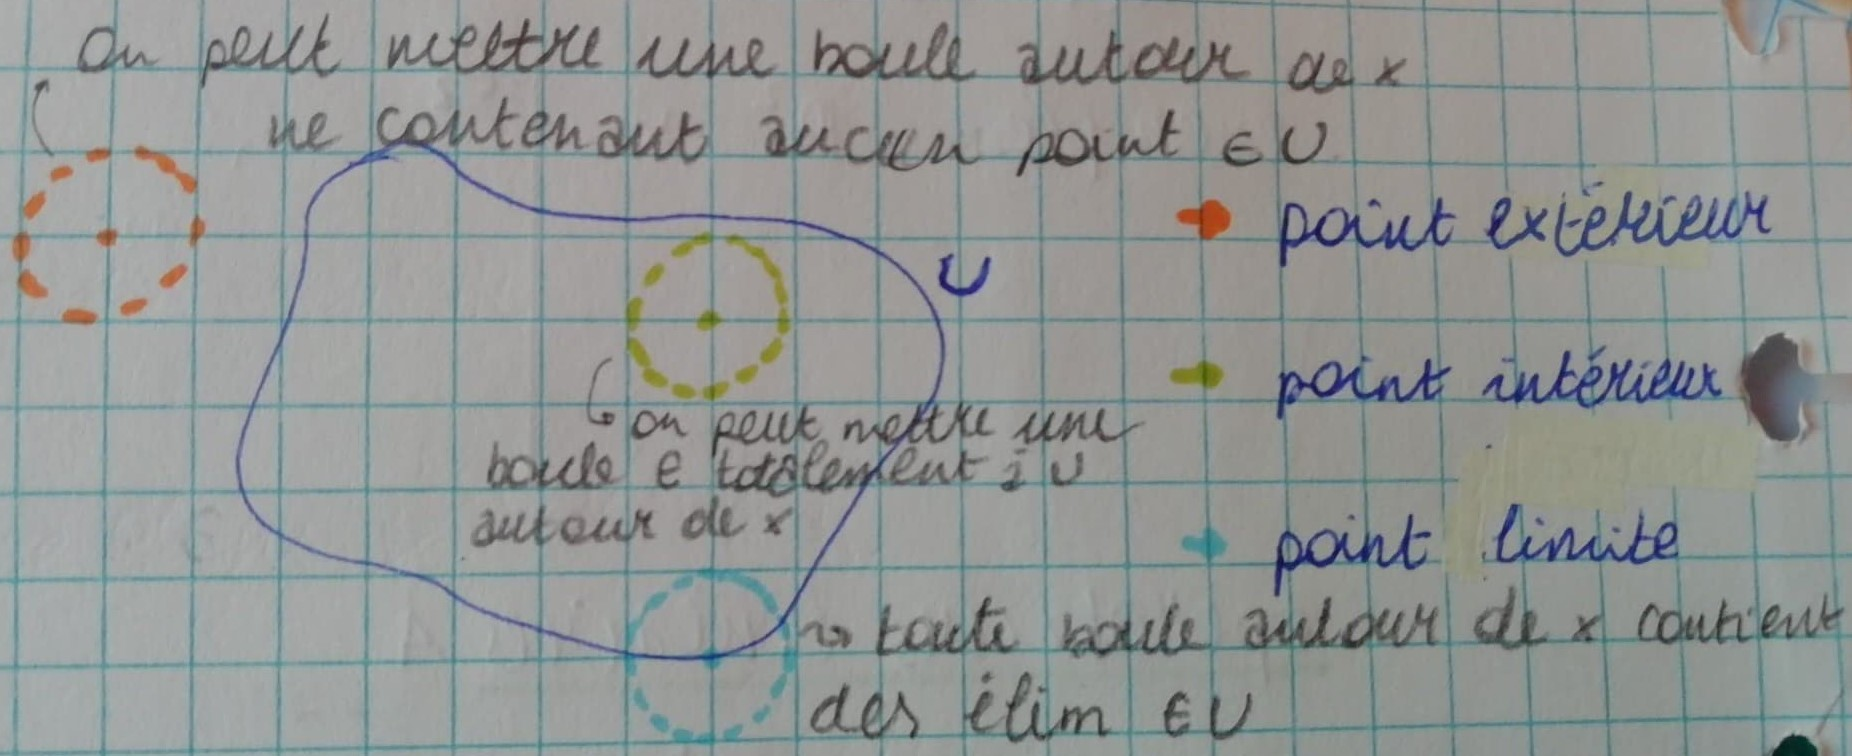
\includegraphics[scale = 0.3]{synthese_BO.jpg}
\end{figure}

\begin{definition}
    Un point $x\in U\subseteq X$ est un \textbf{point intérieur} à $U$ s'il existe $r>0$ tel que $B_r(x) \subseteq U$. De manière équivalente, $x$ est un point intérieur de $U$ si $U$ contient (entièrement !) une certaine balle en $x$.
\end{definition}

\begin{definition}
    Si $x$ est un point intérieur de $U$, alors $U$ est aussi appelé \textbf{voisinage} de $x$ (voisinage de $x$ = boule ouverte centrée en $x$).
\end{definition}

\begin{definition}
    Un point $x$ est appelé \textbf{point limite} de $U$ si $B_r(x)\cap \left(U\setminus \left\{x\right\}\right)\neq\emptyset$ pour toute balle autour de $x$. Notez qu'un point limite n'est pas spécialement un élément de $U$, mais $U$ doit contenir un point arbitrairement proche de $x$.
\end{definition}

\begin{remark}
    Un point intérieur est un point limite mais un point limite n'est pas toujours un point intérieur
\end{remark}

\begin{example}
    Le point $a$ est il point limite de l'ensemble $\{a,b\}$ ? Non car cet espace est un espace discret. Il existe donc une boule ne contenant aucun autre élément que $a$.
\end{example}

\begin{definition}
    Un point $x$ est un \textbf{point isolé} de $U$ s'il existe un voisinage de $x$ ne contenant aucun autre élément de $U$. Un espace contenant que des points isolés est un \textbf{espace discret}.
\end{definition}

\begin{definition}
    Si tout voisinage de $x$ contient au moins un élément de $U$ et un élément hors de $U$, alors $x$ est appelé \textbf{point frontière}. En mathématique, on écrit que $U\subseteq X$ si pour tout $r>0$
    \begin{equation*}
        \left\{\begin{array}{rcl}
            B_r(x)\cap U &\neq& \emptyset  \\
            B_r(x)\cap (X\setminus U) &\neq& \emptyset
        \end{array}\right.
    \end{equation*}
    L'ensemble de tous les points frontière de $U$ est appelé la frontière de $U$ \footnote{Étonnant, n'est-ce pas ?} et dénoté par $\partial U$.
\end{definition}

Un point frontière est-il toujours point limite ? Non. Prenons un point isolé $x$. Ce point est par définition un point frontière mais pas un point limite.

Un point frontière peut-il être point intérieur d'un même ensemble ? Non, car il est possible de trouver une boule (assez petite) en un point intérieur $x\in U\subseteq X$ qui ne contiennent aucun élément de $X \textbackslash U$. Ce point ne peut être point frontière, donc. De même, il est impossible de trouver une boule en un point frontière $y$ qui ne contienne aucun élémenent de $X$.

\begin{definition}
    Un ensemble dont tous les points sont des points intérieurs est appelé \textbf{ensemble ouvert} ; $U \subseteq X$ est \textbf{ouvert} si $\forall x \in U : \exists \ r > 0 : B_r(x) \subseteq U$
    \newpage
    La famille de tous les ensembles ouverts $\mathcal{O} \in$ à l'espace métrique $X$ satisfait les propriétés suivantes :
    \begin{enumerate}[label=(\roman*)]
        \item $\emptyset,X\in \mathcal{O}$ ;
        \item $O_1,O_2\in \mathcal{O}$ implique $O_1\cap O_2 \in \mathcal{O}$ ;
        \item $\left\{ O_\alpha \right\} \subseteq \mathcal{O}$ implique $\bigcup_\alpha O_\alpha \in \mathcal{O}$.
    \end{enumerate}
\end{definition}

\danger \textbf{Attention} :
    \begin{enumerate}[label=(\roman*)]
        \item Une intersection infinie d'ouvert n'est pas toujours un ouvert : $\bigcap \limits^\infty_{n=1}]\frac{-1}{n},1[ = [0,1[$
        \item Une intersection finie d'ouvert est toujours un ouvert
        \item Une union finie d'ouvert est toujours un ouvert
    \end{enumerate}
\vspace{0.3cm}

Un ensemble $X$ auquel est associé une famille $\mathcal{O}$ de sous-ensembles de $X$ qui satisfait les trois propriétés est appelé \textbf{espace topologique} : $(X, \mathcal{O})$ est un espace topologique de l'ensemble $X$ si la topologie $\mathcal{O} \subseteq \mathcal{P}(X)$ sur $X$ satisfait les 3 propriétés.\\

\begin{definition}
    Soit $(X,\mathcal{O})$ un espace topologique. Un ensemble $Y \subseteq X$ est un \textbf{sous-espace topologique} de $X$ s'il est muni de la \textbf{topologie induite}. C'est à dire, qu'un sous-ensemble $Z \subseteq Y$ est ouvert ssi il existe un ouvert $O \subseteq X$ tel que $Z = O \cap Y$.
\end{definition}

\begin{example}
    Soit $\mathbb{R}$ l'ensemble des réels muni de sa topologie naturelle. Soit $Y := [-1,1]$ le sous-espace topologique de $\mathbb{R}$ muni de la topologie induite. Si $Z = ]0,1]$, il suffit par exemple de prendre $O = ]0,a[$ avec n'importe quel réel $a > 1$.
    
    On remarque donc que $Z$ n'est pas un ouvert pour la topologie de $\mathbb{R}$ mais il l'est dans $Y$ pour la topologie induite.
\end{example}

\begin{remark}
    Le fait qu'un ensemble $Z$ soit ouvert ou fermé dans un ensemble $X$ ne dépend pas uniquement de l'ensemble $Z$ lui-même, ça dépend aussi de $X$!
\end{remark}

Les notions de point intérieur, de point limite et de voisinage se répercutent sur les espaces topologiques si nous remplaçons la boule ouverte autour de $x$ par un jeu ouvert contenant $x$. Il existe différents choix quant à la topologie, les plus évidents étant la \textbf{topologie triviale} $\mathcal{O} = \left\{ \emptyset,X \right\}$ et la \textbf{topologie discrète} $\mathcal{O} = \mathcal{P}(X)$.\\

\begin{definition}
    Un espace topologique $(X,\mathcal{O})$ est de \textbf{Hausdorff} si pour tout $x,y \in X$ ($x\neq y$), il existe $O_1,O_2$ tels que $x\in O_1\in \mathcal{O}$ et $y\in O_2\in \mathcal{O}$ avec $O_1\cap O_2=\emptyset$. Autrement dit, pour deux points distincts, il existe deux voisinages disjoints.
\end{definition}

%Dans un tel espace, si une suite a une limite, alors cette limite est unique.

\begin{theo}
    Si $U\subseteq X$ est fermé, alors $X\setminus U$ est ouvert.
\end{theo}

\begin{definition}
    La boule fermée de rayon $r$ centrée en $x$ est donnée par
    \begin{equation*}
        \overline{B_r}(x) := \left\{ y\in X| d(x,y) \leq r \right\}
    \end{equation*}
    Remarquez que $\overline{B_r}(x)$ n'est pas une adhérence !
\end{definition}

\begin{definition}
    Soit $U\subseteq X$ un ensemble. Le plus petit ensemble fermé contenant l'ensemble $U$, appelé \textbf{adhérence} ou \textbf{fermeture} de $U$ et est noté $\overline{U}$. Le plus grand ensemble ouvert contenu dans $U$ est appelé \textbf{intérieur} de $U$ et est noté $U \degree$
    
    Propriétés (démos TP3) :
    \begin{enumerate}[label=(\roman*)]
        \item $\overline \emptyset = \emptyset$,
        \item $U \subseteq \overline U$,
        \item $\overline{\overline U} = \overline U$,
        \item $\overline{U\cup V} = \overline U \cup \overline V$.
        \item $X \setminus \overline{U} = (X \setminus U)\degree$ et $X \setminus U\degree = \overline{X \setminus U}$
        \item $\partial U = \overline{U} \setminus U\degree$
    \end{enumerate}
\end{definition}

\begin{theo}
    \begin{equation*}
        \overline{B_r(x)} \subseteq \overline{B_r}(x).
    \end{equation*}
\end{theo}

\begin{example}
    Soit l'espace métrique $X := \{0,1\}$ muni de la distance $d(x,y) := |x-y|$. On a donc $\overline{B_1^X}(0) = \{0,1\}$ et $B_1^X(0) = \{0\}$. Donc, $\overline{B_1^X(0)} = \overline{\{0\}} = \{0\} \subseteq \{0,1\}$
\end{example}

%\begin{proof}
    %Cela équivaut à prouver que $X\setminus \overline{B_r}(x)\subseteq X\setminus \overline{B_r(x)}$. Prenons par exemple les points $x,y\in\mathbb{R}^2$ sur la Fig.\ref{fig:preuve1} tels que $d(x,y) = R$. Soit $B_r(x)$ la boule ouvert en $x$ de rayon $r<R$.
    %\begin{figure}
        %\centering
        %\tikzsetnextfilename{preuve1}
        %\begin{tikzpicture}
            %\draw[->] (-.5,0) -- (4,0) node[below] {\small{$e_1$}};
            %\draw[->] (0,-.5) -- (0,4) node[left] {\small{$e_2$}};

            %\draw plot[mark=*, mark size=.3mm] (1.6,1.3) node[above left] {\small{$x$}} circle(1) -- (2.3071,2.0071) node[above right] {\small{$r$}};
            %\draw (1.6,1.3) -- (3,1.7) node[above left] {\small{$R$}} -- plot[mark=*, mark size=.3mm] (3.6,1.9) node[above right] {\small{$y$}};
        %\end{tikzpicture}
        %\caption{}
        %\label{fig:preuve1}
    %\end{figure}
%\end{proof}

%\begin{theo}
    %Une famille d'ensembles ouverts $\mathcal{B}\subseteq\mathcal{O}$ est une \textbf{base} pour la topologie si et seulement si tous les ensembles ouverts peuvent être écrits comme une union des éléments de $\mathcal{B}$.
%\end{theo}

\subsection{Convergence}

\begin{definition}
    Une \textbf{sous-suite} (ou une \textbf{suite extraite}) d'une suite $(x_n)_{n\in\mathbb{N}}$ est une suite $(x_{n_k})_{k\in\mathbb{N}}$ où $(n_k)_{k\in\mathbb{N}}\subset \mathbb{N}$ est strictement croissante.
\end{definition}

\begin{definition}
    Dans un espace métrique $(X,d)$, la suite $(x_n)_{n\in\mathbb{N}}\subset X$ est \textbf{bornée} si et seulement si $\sup_{n\in\mathbb{N}}d(x_n,x_0)<\infty$. Autrement dit, $(x_n)_{n\in\mathbb{N}}\subset X$ est bornée si $\exists y \in X, r > 0 : \forall n \in \mathbb{N} : x_n \in B_r(y)$. 
\end{definition}

\begin{definition}
    Dans un espace métrique $(X,d)$, une suite $(x_n)_{n=1}^\infty$ \textbf{converge} vers un point $x\in X$ si $\lim \limits_{n\rightarrow\infty}d(x,x_n) = 0$. De manière équivalente, on dit qu'une suite $x_n$ converge si et seulement s'il existe $x\in X$ tel que pour tout réel $\epsilon>0$, il existe $N\in\mathbb{N}$ tel que $d(x_n,x) \leq \epsilon$ (ou $x_n \in B_\epsilon(x)$) pour tout entier $n\geq N$. Il semble évident que cette limite est unique, si elle existe.
\end{definition}

\begin{definition}
    Soit une suite $(u_n)_{n \in \mathbb{N}}$ de fonctions d’un ensemble $X$ dans un espace métrique $(Y, d)$.
    
    La suite \textbf{converge ponctuellement} vers $u(x)$ si
    \begin{equation*}
        \exists u : X \rightarrow Y \ \text{telle que} \lim \limits_{n\to\infty} d(u_n(x), u(x)) = 0 \quad \forall x \in X
    \end{equation*}
    
    
    La suite \textbf{converge uniformément} vers $u(x)$ si
    \begin{equation*}
        \exists u : X \rightarrow Y \ \text{telle que} \lim \limits_{n\to\infty} \sup \limits_{x \in X} \{d(u_n(x), u(x))\} = 0
    \end{equation*}
    
    La convergence uniforme implique la convergence ponctuelle mais pas le contraire
\end{definition}

\noindent
\fbox{\parbox{\textwidth}{%\raggedleft
    \begin{exo}
        Soit $(x_n)_{n\in\mathbb{N}}$ une suite de nombres réels décroissante et bornée. Prouver que $(x_n)_{n\in\mathbb{N}}$ converge et
        \begin{equation*}
            \lim_{n\to\infty}x_n = \inf\{x_n:n\in\mathbb{N}\}
        \end{equation*}
    \end{exo}
    \begin{sol}
        Soit $N = \inf\{x_n:n\in\mathbb{N}\}$. Comme la suite est bornée, nous déduisons que $N\in\mathbb{R}$ existe. La suite étant décroissante, nous avons $d(x_n,N) \geq d(x_m,N)$, $\forall m > n$. En choisissant $\epsilon = d(x_n,N) > 0$, on peut affirmer que la suite converge uniformément vers $N$.
    \end{sol}
}}\\

\begin{theo}[Bolzano-Weierstrass]
    Tout suite bornée admet une sous-suite convergente. (démo au TP2) \danger Pas valable en dimension infinie !
\end{theo}

Il est à noter qu'une suite convergente est bornée. Un ensemble $U\subset X$ est \textbf{borné} s'il est contenu dans une balle, c'est-à-dire $U\subset B_r(x)$ pour certains $x\in X$ et $r>0$. \\

%Une métrique induit naturellement une topologie et une topologie induit naturellement une notion de convergence. Cependant, une notion de convergence peut ne pas provenir d'une topologie (ou différentes topologies peuvent donner lieu à la même notion de convergence) et une topologie peut ne pas provenir d'une métrique.

\begin{definition}
    Une suite $(x_n)_{n=1}^\infty\in X^\mathbb{N}$ est appelée \textbf{suite de Cauchy} si pour chaque $\epsilon>0$, il existe $N\in\mathbb{N}$ tel que
    \begin{equation*}
        d(x_n,x_m)\leq\epsilon,\qquad n,m\geq N.
    \end{equation*}
\end{definition}

\begin{theo}
    Toute suite convergente est de Cauchy.
\end{theo}

\noindent
\fbox{\parbox{\textwidth}{%\raggedleft
    \begin{exo}
        Démontrer que dans un espace métrique, toute suite de Cauchy est bornée.
    \end{exo}
    \begin{sol}
        Soit la suite $(u_n)_{n=1}^\infty$ qui converge uniformément vers $u$. On a alors, par inégalité triangulaire, que
        \begin{equation*}
            0\leq d(u_j,u_k)\leq d(u_j,u) + d(u,u_k)
        \end{equation*}
        et $\lim \limits_{j,k\to\infty} d(u_j,u_k) = 0$. Si cette suite est de Cauchy, pour un certain $\epsilon>0$, il existe alors $m\in\mathbb{N}$ tel que $j,k\geq m$ et $d(u_j,u_k)\leq\epsilon$. On obtient alors pour tout $n$
        \begin{equation*}
            d(u_0,u_n) \leq \max\{ d(u_0,u_1), \cdots , d(u_0,u_{m-1}), d(u_0,u_m)+\epsilon \}.
        \end{equation*}
    \end{sol}
}}\\

\begin{definition}
    Une suite $(x_n)_{n\in\mathbb{N}}$ de nombres réels est \textbf{sommable} si la suite $\Big(\sum \limits_{k=0}^n x_k\Big)_{n\in\mathbb{N}}$ converge.
\end{definition}

\begin{definition}
    La limite $\lim \limits_{n\to\infty}\sum \limits_{k=0}^n x_k = \sum \limits_{k=0}^\infty x_k$ est appelée \textbf{somme} de la série de terme $x_n$.
\end{definition}    

\begin{definition}
    $\sum \limits_{k=0}^\infty x_k$ converge si la suite $(x_n)_{n\in\mathbb{N}}$ est sommable. Dans le cas contraire, la série est dite \textbf{divergente}.\\
    
    Les définitions de convergence ponctuelle et uniforme restent valables pour les séries en regardant la convergence de la suite $\Big(\sum \limits_{k=0}^n x_k\Big)_{n\in\mathbb{N}}$\\
    
    La série $\sum \limits_{k=0}^n x_k$ où $(x_k)_{k\in\mathbb{N}}$ est une suite de Y dans un espace normé (cf plus loin) \textbf{converge absolument ponctuellement} si
    \begin{equation*}
         \sum \limits_{k=0}^n ||x_k(y)|| < \infty \quad \forall y \in Y
    \end{equation*}
    
    La série $\sum \limits_{k=0}^n x_k$ où $(x_k)_{k\in\mathbb{N}}$ est une suite de Y dans un espace normé (cf plus loin) \textbf{converge normalement} si
    \begin{equation*}
         \sum \limits_{k=0}^n \sup \limits_{y \in Y}||x_k(y)|| < \infty
    \end{equation*}
    
    La convergence normale implique la convergence absolue ponctuelle.
\end{definition}

\subsection{Caractérisation des fermés}

$U\subseteq X$ est fermé si pour toute suite $(x_n)_{n=1}^\infty\subseteq U$ et $x_n\rightarrow x$, alors $x\in U$.

\begin{definition}
    Un espace métrique $X$ est \textbf{complet} si toute suite de Cauchy converge avec limite dans $X$.
\end{definition}

\noindent
\fbox{\parbox{\textwidth}{%\raggedleft
    \begin{exo}
        Prouver que $\mathbb{Q}$ muni de la distance $d(x,y)=|x-y|$ n'est pas complet.
    \end{exo}
    \begin{sol}
        Considérons la suite $(x_n)_{n\in\mathbb{N}}$ définie par
        \begin{equation*}
            x_0=2,\quad x_{n+1} = \frac{1}{2}\left(x_n + \frac{2}{x_n}\right)
        \end{equation*}
        Prouvons d'abord que cette suite est de Cauchy. Pour ce faire, étudions la suite afin de voir si elle croissante ou décroissante :
        \begin{equation*}
            x_{n+1} - x_n = \frac{2-x_n^2}{x_n} \overset{?}{\gtrless} 0
        \end{equation*}
        On en déduit que la fonction est décroissante positive et qu'elle converge vers $\sqrt{2}$, c'est-à-dire dans $\mathbb{R}$. On en conclut que $\mathbb{R}$ est complet, mais pas $\mathbb{Q}$.
    \end{sol}
}}\\

\begin{lemme}
    Soit $X$ un espace métrique complet et $U\subseteq X$. On a :
    \begin{equation*}
        U\ \mathrm{complet} \quad\Longleftrightarrow\quad U\ \mathrm{ferm\acute{e}}
    \end{equation*}
\end{lemme}

\begin{definition}
    L'espace métrique $U\subseteq X$ est \textbf{dense} si et seulement si $\overline{U}=X$. Autrement dit, $U$ est dense dans $X$ ssi $\forall x \in X, \forall r>0 : B_r(x) \cap U \neq \emptyset$
\end{definition}

\begin{lemme}
    L'espace métrique $X$ est \textbf{séparable} si et seulement s'il contient un ensemble dense dénombrable.
\end{lemme}

\begin{example}
    $\mathbb{Q}$ est dense dans $\mathbb{R}$ (imaginons une infinité de frontières entre chaque éléments de $\mathbb{Q}$). L'ensemble $\mathbb{Q}$ est également dénombrable. On a donc que $\mathbb{R}$ est séparable.
\end{example}

\subsection{Fonctions}

\begin{definition}
    une fonction $f$ est la relation d'un ensemble $X$ vers un ensemble $Y$ pour laquelle chaque élément $x\in X$ est en relation avec un unique élément du second, appelé image de $x$ et noté $f(x)$. C'est-à-dire
    \begin{equation*}
        f:X\rightarrow Y,\ x\mapsto f(x).
    \end{equation*}
    On écrit généralement $f(U) = \left\{ f(x)|x\in U \right\}$ pour $U\subseteq X$ et $f^{-1}(V) = \left\{ x|f(x)\in V \right\}$ pour $V\subseteq Y$.
\end{definition}

\begin{figure}[H]
    \centering
    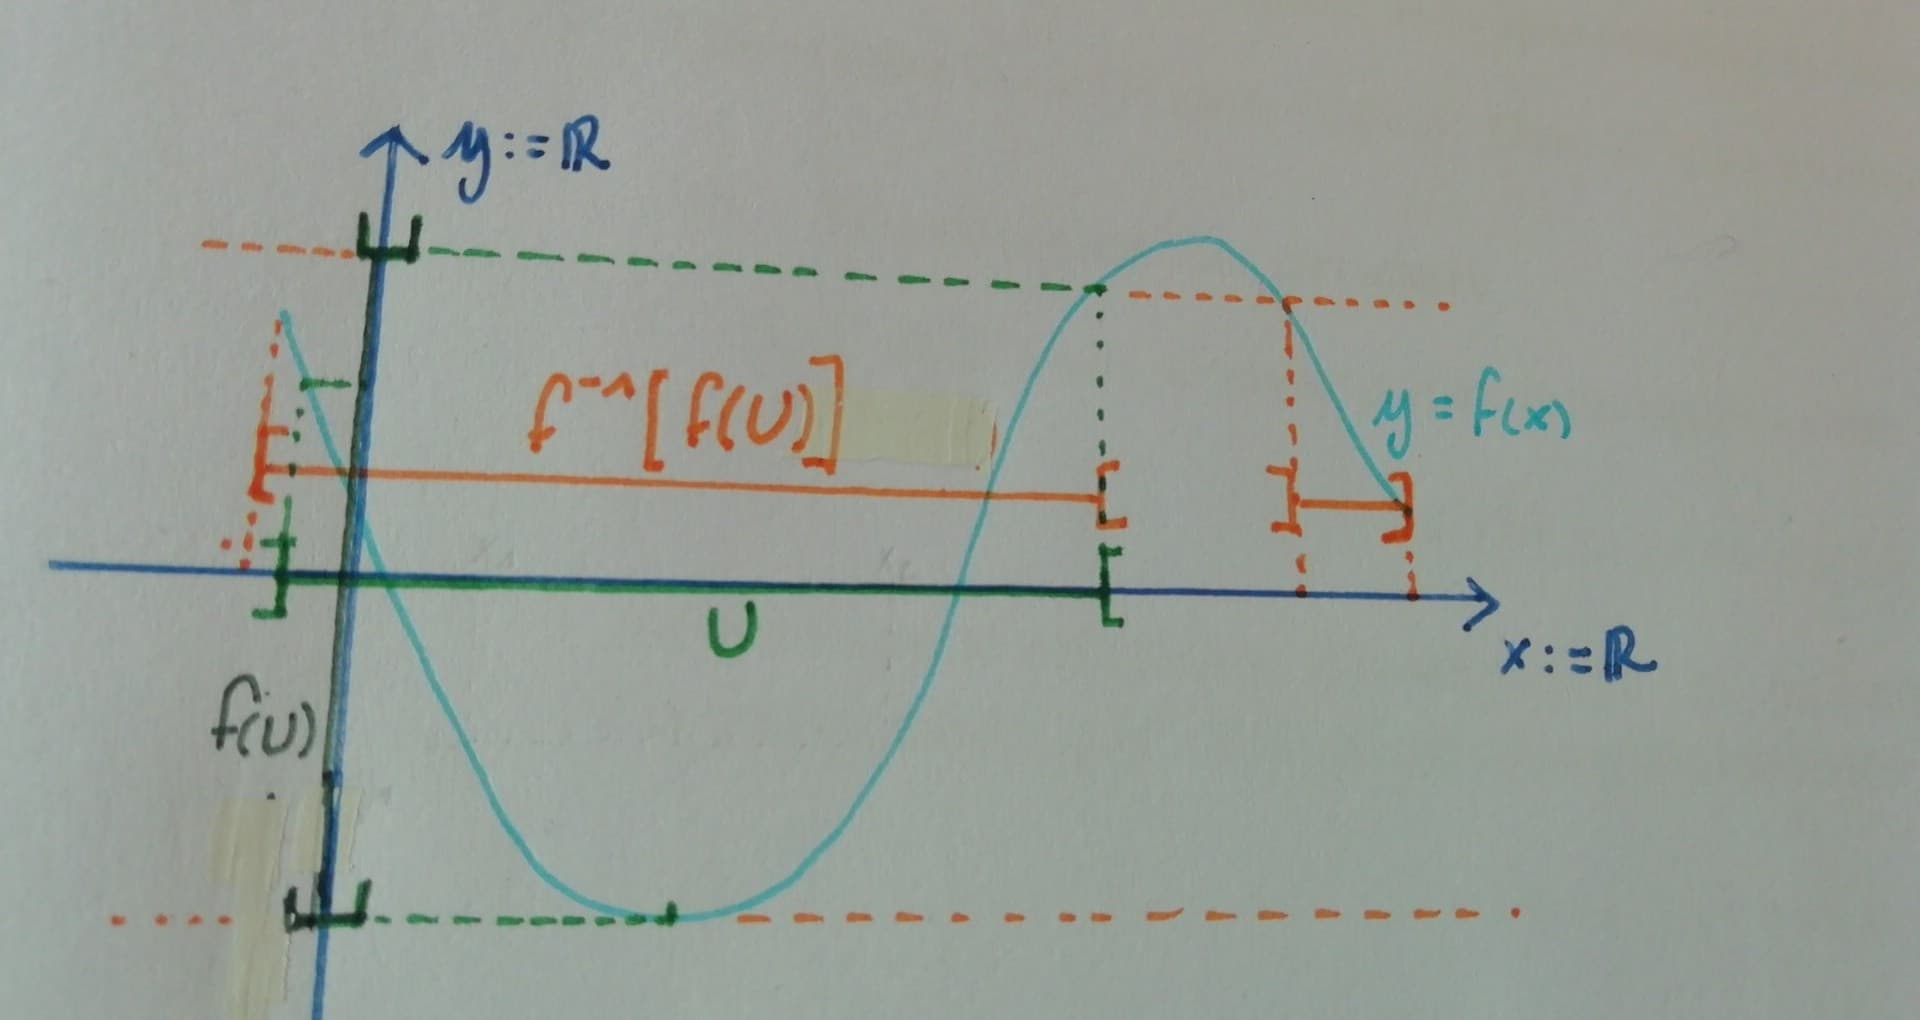
\includegraphics[scale = 0.1]{synthese_fct.jpg}
\end{figure}

\begin{definition}
    On dit qu'une fonction $f$ est
    \begin{itemize}
        \item \textbf{injective} si pour chaque $y \in Y$, il y a au plus un $x \in X$ tel que $f(x) = y$ ($f^{-1}(y)$ contient au plus un point);
        \item \textbf{surjective} si $f(X)=Y$;
        \item \textbf{bijective} si elle est à la fois injective et surjective.
    \end{itemize}
\end{definition}

\begin{definition}

    Une fonction $f$ entre deux espaces métriques $X$ et $Y$ est dite continue en un point $x\in X$ si pour tout $\epsilon>0$, on peut trouver un $\delta>0$ tel que $d_Y(f(x),f(y)) \leq \epsilon \quad\mathrm{si}\quad d_X(x,y)<\delta$ ou de manière équivalente : $f(B_\delta(x)) \subseteq B_\epsilon(f(x))$.\\
    \begin{figure}[H]
        \centering
        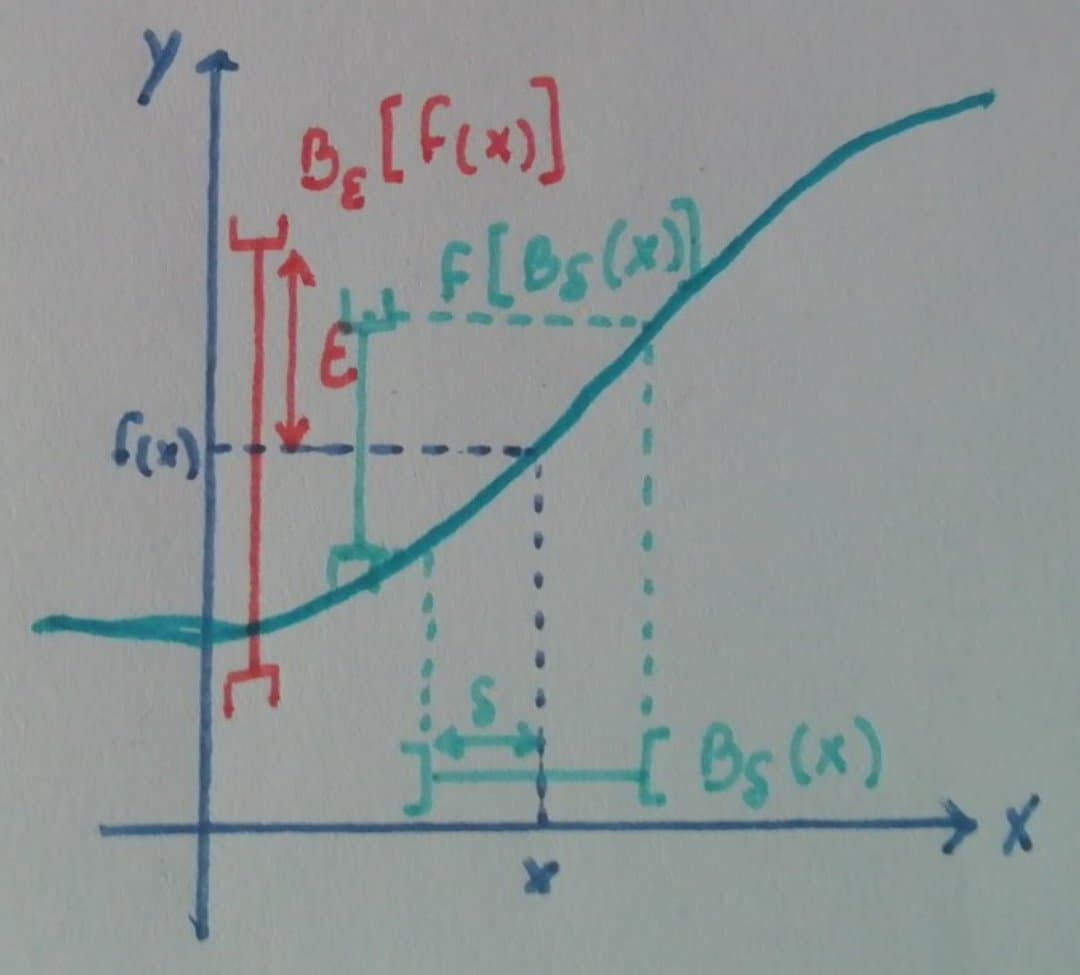
\includegraphics[width=0.3\textwidth]{synthese_continuite.jpg}
    \end{figure}
    Si $f$ est continue en chaque point, on dit qu'elle est \textbf{continue}.
\end{definition}

\begin{definition}
    Une fonction $f:X \rightarrow Y$ avec $X$ et $Y$ deux espaces métriques muni des distance $d_X$ et $d_Y$ respectivement est \textbf{uniformément continue} si $\forall \epsilon>0, \exists \delta>0$ tels que $\forall x,y \in X : d_X(x,y) \leq \delta \implies d_Y(f(x),f(y))\leq \epsilon$.
\end{definition}

\begin{theo}
    Soient $X,Y$ deux espaces métriques. Les déclarations suivantes sont équivalentes :
    \begin{enumerate}[label=(\roman*)]
        \item $f$ est continue en $x$ ;
        \item $f(x_n)\rightarrow f(x)$ pour n'importe quel $x_n \rightarrow x$ ;
        \item Pour tout voisinage $V$ de $f(x)$, la pré-image $f^{-1}(V)$ est un voisinage de $x$.
    \end{enumerate}
\end{theo}

\begin{proof}

    $1.\Rightarrow2.$ Soit un réel $\epsilon>0$. Par continuité de $f$, il existe $\delta>0$ tel que $f(B_\delta(x))\subseteq B_\epsilon(f(x))$. Par convergence de $(x_n)$ vers $x$, il existe $N$ tel que $\forall n\geq N$ :
    \begin{equation*}
        x_n\in B_\delta(x) \Rightarrow f(x_n)\in f(B_\delta(x)) \subseteq B_\epsilon(f(x))
    \end{equation*}
    
    $2.\Rightarrow3.$ Par contradiction : Soit $V$ un voisinage de f(x) tel que $f^{-1}(V)$ n'est pas un voisinage de $x$ ($\forall \delta > 0: B_\delta(x) \not\subseteq f^{-1}(V)$). Dans ce cas, on peut choisir une suite $x_n \in B_{\frac{1}{n}}(x)$ qui converge vers $x$ telle que $f(x_n) \notin V$ et donc $f(x_n) \nrightarrow f(x)$.\\
    \begin{figure}[H]
        \centering
        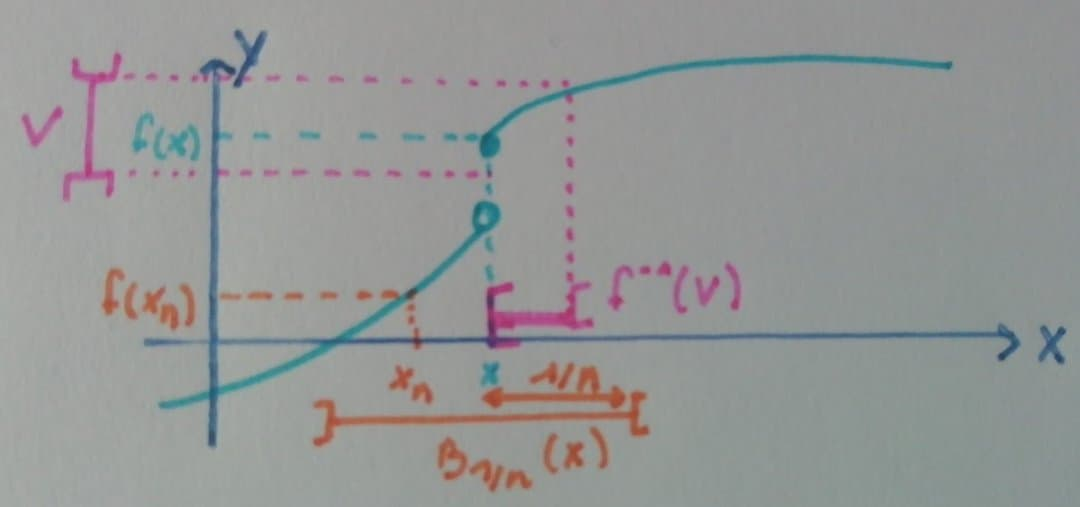
\includegraphics[scale = 0.2]{synthese_continuite_theo.jpg}
    \end{figure}
    
    $3.\Rightarrow1.$ Soit un voisinage V autour de $f(x)$ : $V = B_\epsilon(f(x))$, $\epsilon > 0$. Dès lors, $f^{-1}(V) = f^{-1}(B_\epsilon(f(x)))$ est un voisinage de x donc $\exists\delta : B_\delta(x)\subseteq f^{-1}(B_\epsilon(f(x)))$, c'est-à-dire que $f$ est continue en $x$.
\end{proof}

\begin{remark}
	$f:X\rightarrow Y$ est continue si et seulement si $\forall \mathcal{O}$ ouvert de $Y:f^{-1}(\mathcal{O})$ est un ouvert de $X$.
\end{remark}

%\begin{definition}
	%La fonction $f$ est un \textbf{homéorphisme} si et seulement si elle est bijective et que $f$ et $f^{-1}$ sont continues.
%\end{definition}

\begin{definition}
    Le \textbf{support} de la fonction f est défini comme
	\begin{equation*}
		\text{supp}(f):=\overline{\{x\in X|f(x)\neq0\}}
	\end{equation*}
\end{definition}

\subsection{Compacité}

\begin{definition}
	Un \textbf{recouvrement} de $Y\subseteq X$ est une famille d'ensembles $\{U_\alpha\}_{\alpha\in A}$ telle que $Y\subseteq \bigcup_{\alpha\in A}U_\alpha$. Le recouvrement est \textbf{ouvert} si tous les $U_\alpha$ sont ouverts. Un \textbf{sous-recouvrement} est une sous-famille de $\{U_\alpha\}$ qui reste un recouvrement de $Y$. 
\end{definition}

\begin{figure}[H]
    \centering
    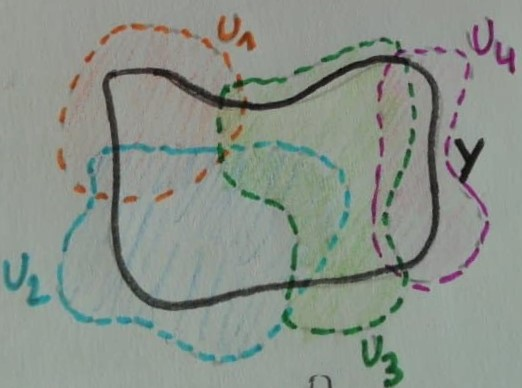
\includegraphics[scale = 0.4]{synthese_recouvrement.jpg}
\end{figure}

\begin{definition}
    Un ensemble $K\subseteq X$ est \textbf{compact} si \underline{tout} recouvrement \textit{ouvert} de $K$ a un sous-recouvrement fini. (Un espace est non compact si il est trop grand ex. $\mathbb{R}$)
\end{definition}

\begin{theo}
    Soit un espace topologique $X$.
    \begin{enumerate}[label=(\roman*)]
        \item L'image continue d'un ensemble compact est compacte.
        \item Tout sous-ensemble fermé d'un ensemble compact est compact.
        \item Si $X$ est de Hausdorff, tout ensemble compact est fermé.
    \end{enumerate}
\end{theo}

\begin{proof}
    \begin{enumerate}
        \item Observons que si $\{O_\alpha\}$ est un recouvrement fermé de $f(Y)$, alors $\{f^{-1}(O_\alpha)\}$ en est un pour $Y$.
        \begin{figure}[H]
            \centering
            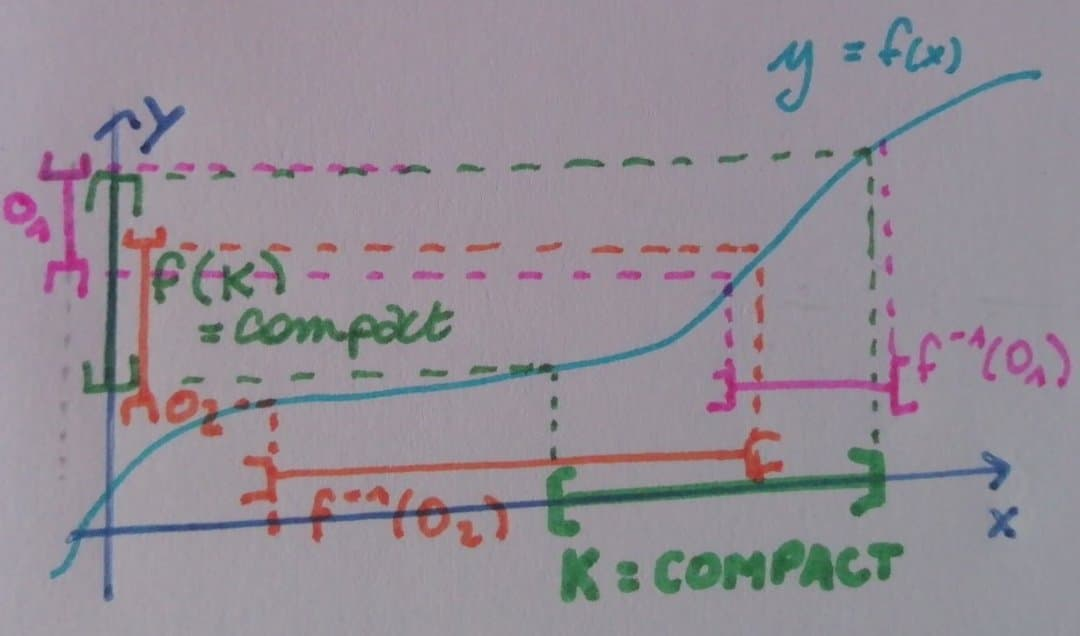
\includegraphics[scale = 0.2]{synthese_compact.jpg}
        \end{figure}
        \item Soit $\{O_\alpha\}$ un recouvrement ouvert d'un sous-ensemble fermé $Y$. Alors, il existe des ensembles ouverts $\tilde{O}_\alpha$ avec $O_\alpha = \tilde{O}_\alpha\cap Y$ et $\{\tilde{O}_\alpha\}\cup\{X\setminus Y\}$ (un recouvrement ouvert de $X$) qui sont un sous-recouvrement fini. Ce sous-recouvrement implique un sous-recouvrement fini de $Y$.
        \item Soit $Y\subseteq X$ un compact. On montre que $X\setminus Y$ est ouvert. Fixons $x\in X\setminus Y$. Comme l'ensemble $X$ est de Hausdorff, pour chaque $y\in Y$ (donc $\in X$), il y a un voisinage disjoint $V(y)$ de $y$ et $U_y(x)$ de $x$. Comme $Y$ est compact, il existe $y_1,\cdots,y_n$ tels que $V(y_j)$ recouvre $Y$. Mais alors $\bigcap_{j=1}^n U_{y_j}(x)$ est un voisinage de $x$ qui n'a aucune intersection avec $Y$.
    \end{enumerate}
\end{proof}

\begin{definition}
    L'ensemble $K\subseteq X$ est \textbf{séquentiellement compact} si toute suite dans $K$ a au moins une sous-suite convergente dont la limite est dans $K$.
\end{definition}

\begin{definition}
    L'ensemble $K\subseteq X$ est \textbf{séquentiellement fermé} si toute suite dans $K$ converge dans $K$.
\end{definition}

\begin{theo}
    Tout ensemble $K\subseteq X$ est compact (fermé) si et seulement s'il est séquentiellement compact (fermé).
\end{theo}

\begin{theo}
    Un espace métrique compact est complet et séparable.
\end{theo}

\begin{theo}
    Un espace métrique compact est fermé et borné (démo TP8).
\end{theo}

\begin{theo}[Heine-Borel]
    Dans $\mathbb{R}^n$, un ensemble est compact si et seulement s'il est fermé et borné.
\end{theo}

\subsection{Topologies du produit}

Si $X$ et $Y$ sont deux espaces métriques, alors $X\times Y$ associé à \[d((x_1,y_1),(x_2,y_2)) := d_X(x_1,x_2) + d_Y(y_1,y_2)\] est un espace métrique. Une suite $(x_n,y_n)_{n \in \mathbb{N}}$ converge vers $(x,y)$ si et seulement si $x_n\rightarrow x$ et $y_n\rightarrow y$. En particulier, par l'inégalité triangulaire inverse, on a \[|d(x_n,y_n) - d(x,y)| \leq d(x_n,x) + d(y_n,y)\] on voit que $d:X\times X \rightarrow \mathbb{R}$ est continue.

\part{Analyse fonctionnelle}

%\sectionmark{}
%\sectionmark{Espaces de Banach et de Hilbert}
\section{Premiers pas avec les espaces de Banach et de Hilbert}
\sectionmark{Premiers pas}

\subsection{Espaces de Banach pour des fonctions continues}
% Sous section 2.1

Notre point de départ sera l'ensemble des fonctions continues $C(I)$ sur un intervalle compact $I := \left[ a,b \right] \subset \mathbb{R}$.

Une manière de déclarer une distance est la \textbf{norme maximale} :
\begin{equation*}
    ||f||_\infty := \max_{x\in I}|f(x)|.
\end{equation*}
Et il devient évident que $C(I)$ devient un espace vectoriel normé.

\begin{definition}
    Un \textbf{espace vectoriel normé $X$} est un espace vectoriel $X$ sur $\mathbb{C}$ (ou $\mathbb{R}$) auquel est associé une fonction positive $||\cdot||:X \rightarrow \mathbb{C}:f \rightarrow ||f||$ telle que
    \begin{enumerate}[label=(\roman*)]
        \item $||f||>0$ pour $f\neq0$ (définie positive),
        \item $||\alpha f|| = |\alpha|\ ||f||$ pour tout $\alpha\in\mathbb{C}$, $f\in X$ (homogénéité positive) et
        \item $||f+g||\leq||f||+||g||$ pour tout $f,g\in X$ (inégalité triangulaire).
    \end{enumerate}
\end{definition}

\begin{remark}
    Soit $(X,||\cdot||)$ un espace vectoriel normé. Alors $(X,d)$ où $d(f,g):=||f-g||$ est un espace métrique.
\end{remark}

Par conséquent, on sait que quand une suite de vecteur $f_n$ converge vers un vecteur $f$ on a $d(f_n,f)\underset{n\to\infty}{\longrightarrow} 0$. On peut donc aussi dire que la suite $f_n$ converge vers $f$ si $||f_n-f|| \underset{n\to\infty}{\longrightarrow} 0$. On écrira alors que $f_n\rightarrow f$ ou $\lim \limits_{n\to\infty} f_n = f$.

\begin{theo}[Inégalité triangulaire inverse]
    \begin{equation*}
        \bigg| ||f||-||g|| \bigg| \leq ||f-g||
    \end{equation*}
\end{theo}

\begin{remark}
    Soit $F:X\rightarrow\mathbb{R}$ avec $X$ un espace métrique. Si $|F(x)-F(\hat x)|\leq d(x,\hat x)$ pour tout $x,\hat x\in X$, alors $F$ est \textit{continue}.
\end{remark}

\begin{theo}
    La fonction $||\cdot||:X\rightarrow\mathbb{R}$ est continue.
\end{theo}

\begin{proof}
    \begin{equation*}
        \bigg| ||f||-||g|| \bigg| \leq ||f-g|| = d(f,g).
    \end{equation*}
\end{proof}

%\begin{theo}
    %La fonction $||\cdot||:X\rightarrow\mathbb{R}$ est connexe.
%\end{theo}

%En plus du concept de convergence, nous avons également le concept d'une \textbf{suite de Cauchy} et par conséquent le concept de complétude : un espace normé est dit \textbf{complet} si chaque suite de Cauchy accepte une limite. Un espace normé complet est appelé \textbf{espace de Banach}.

\begin{definition}
    Un \textbf{espace de Banach} est un espace vectoriel normé complet.
\end{definition}

\begin{example}
    L'espace $l^1(\mathbb{N}) = \{a \in \mathbb{R}^\mathbb{N}:||a||_1<\infty\}$ de toutes les suites de valeurs réelles $a=(a_j)_{j=1}^\infty$ pour lesquelles la norme
    \begin{equation*}
        ||a||_1 := \sum_{j=1}^\infty|a_j|
    \end{equation*}
    est finie est un espace de Banach.
\end{example}

\begin{proof}
    Pour le montrer, nous devons vérifier trois choses : (i) $l^1(\mathbb{N})$ est un espace vectoriel qui est fermé sous addition et multiplication scalaire, (ii) $||\cdot||_1$ satisfait les trois conditions requises d'une norme, et (iii) $l^1(\mathbb{N})$ est complet.\\
    
    (i)$\&$(ii) $\sum \limits_{j=1}^k |a_j+b_j| \leq \sum \limits_{j=1}^k |a_j| + \sum \limits_{j=1}^k |a_j+b_j| \leq ||a||_1 + ||b||_1$ avec $k < \infty$. En faisant tendre $k$ vers l'infini, on observe que l'inégalité triangulaire est satisfaite et que $l^1(\mathbb{N})$ est fermé sous l'addition.
    
    Le fait que la norme 1 est définie positive et satisfait la propriété d'homogénéité positive est direct. Dès lors $l^1(\mathbb{N})$ est fermé sous la multiplication.\\
    
    (iii) Soit $(a^n)_{n\in\mathbb{N}}$ une suite de Cauchy dans $l^1(\mathbb{N})$. Dès lors, $\forall \epsilon>0,\exists N_\epsilon$ tq $||a^m-a^n||_1 \leq \epsilon$ pour $m,n \geq N_\epsilon$.
    
    Donc, pour un nombre $j$ fixé, on a $|a_j^m-a_j^n|\leq\epsilon$ car $|a_j^m-a_j^n| \leq ||a^m-a^n||_1$. Donc la suite $(a^n_j)_{n\in\mathbb{N}}$ est une suite de Cauchy. Or l'ensemble $\mathbb{R} \ni a_j^n$ est complet donc on sait que la suite de Cauchy $(a^n_j)_{n\in\mathbb{N}}$ converge et $\lim \limits_{n\to\infty} a_j^n := a_j$.
    
    Considérons maintenant $\sum \limits_{j=1}^{k} |a_j^m - a_j^n| \leq \epsilon$ avec $m\rightarrow\infty$ : $\sum \limits_{j=1}^{k} |a_j - a_j^n| \leq \epsilon$. Cette inéquation étant valable pour tout $k < \infty$, on a $||a-a^n||_1\leq\epsilon$. Donc $(a-a^n) \in l^1(\mathbb{N})$ et on sait que $a^n \in l^1(\mathbb{N})$ : $a=a^n+(a-a^n) \in l^1(\mathbb{N})$. On conclut donc que la suite $(a^n)_{n\in\mathbb{N}}$ converge vers $a$.
\end{proof}

\begin{example}
    L'exemple précédent peut être généralisé en considérant l'espace $l^p(\mathbb{N})$ de toutes les suites de valeurs complexes $a=(a_j)_{j=1}^\infty$ pour lesquelles la norme $p \in [1,\infty[$ est est finie.
    \begin{figure}[H]
        \centering
        \tikzsetnextfilename{produit_cartesien} 
        \begin{tikzpicture}
            \draw[->] (0,-.5) -- (0,2.5);
            \draw[->] (-.5,0) -- (4,0);
            \draw plot[mark=*, mark size=.3mm] (.5,0) -- plot[mark=*, mark size=.3mm] (.5,2) node[above] {$a_1$};
            \draw plot[mark=*, mark size=.3mm] (1,0) -- plot[mark=*, mark size=.3mm] (1,-.6) node[below] {$a_2$};
            \draw plot[mark=*, mark size=.3mm] (1.5,0) -- plot[mark=*, mark size=.3mm] (1.5,.4)  node[above] {$a_3$};
            \draw plot[mark=*, mark size=.3mm] (2,0) -- plot[mark=*, mark size=.3mm] (2,1.3) node[above] {$a_4$};
            \draw (3,0) node[below] {$\cdots$};
            \draw (-.5,1) node[left] {$l^p(\mathbb{N}) \ni$};
            \draw (6,1) node[right] {$||a||_p := \left(\sum|a_n|^p\right)^{1/p} < \infty$};
            
            \draw[->] (0,-4) -- (0,-1);
            \draw[->] (-.5,-2.5) -- (4,-2.5);
            \draw plot[mark=*, mark size=.3mm] (.5,-2.5) -- plot[mark=*, mark size=.3mm] (.5,-2);
            \draw plot[mark=*, mark size=.3mm] (1,-2.5) -- plot[mark=*, mark size=.3mm] (1,-1.5);
            \draw plot[mark=*, mark size=.3mm] (1.5,-2.5) -- plot[mark=*, mark size=.3mm] (1.5,-3.2);
            \draw plot[mark=*, mark size=.3mm] (2,-2.5) -- plot[mark=*, mark size=.3mm] (2,-2.8);
            \draw[dashed] (-.5,-1.5) -- (3.8,-1.5) node[right] {$||a||_\infty$};
            \draw[dashed] (-.5,-3.5) -- (3.8,-3.5) node[right] {$-||a||_\infty$};
            \draw (3,-2.5) node[below] {$\cdots$};
            \draw (-.5,-2.5) node[left] {$l^\infty(\mathbb{N}) \ni$};
            \draw (6,-2.5) node[right] {$||a||_\infty := \mathrm{sup}_{n\in\mathbb{N}} |a_n|_{<\infty}$};
        \end{tikzpicture}
    \end{figure}
\end{example}

\begin{figure}[H]
    \centering
    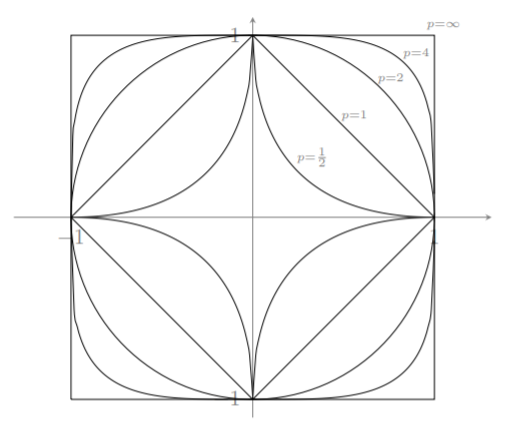
\includegraphics[scale = .5]{unitball.png}
    \caption{Balle unité pour $||\cdot||_p$ dans $\mathbb{R}$}
    \label{fig:unitball}
\end{figure}

\begin{remark}
    La norme $p$ avec $p \in [0,1[$ n'est pas une norme car l'inégalité triangulaire n'est pas satisfaite.
\end{remark}

\begin{remark}
    Toute norme est une fonction CONVEXE. On observe bien sur la figure \ref{fig:unitball} que la fonction $\{a:||a||_{p=0.5}\}$ est concave et que $\{a:||a||_{p\geq1}\}$ sont convexes.
\end{remark}

\vspace{0.5cm}
Du coup, quid de la \textbf{complétude de $C(I)$} ?
%Une suite de fonctions $f_n(x)$ converge vers $f$ si et seulement si
%\begin{equation}
    %\lim_{n\rightarrow \infty}||f-f_n||_\infty = \lim_{n\rightarrow \infty}\sup_{x\in I}|f(x) - f_n(x)| = 0 \qquad \text{(on s'intéresse à $C(I)$ muni de la norme $||\cdot||_\infty$)}.
%\end{equation}
%Maintenant, ayant en tête le cas où $f_n$ est une suite de Cauchy seulement. Alors $f_n(x)$ est une suite de Cauchy de nombres complexes pour tout $x\in I$ fixé. En particulier, par complétude de $\mathbb{C}$, il existe une limite $f(x)$ pour chaque $x$. On obtient donc une fonction $f(x)$ limitée et quand $m\rightarrow\infty$, on voit que l'inégalité de Cauchy se transforme :
%\begin{equation}
    %|f(x)-f_n(x)|\leq\epsilon \quad \forall n>N_\epsilon,\ x\in I.
%\end{equation}

\begin{theo}
    $C(I)$ avec une norme maximale est un espace de Banach.
\end{theo}

\begin{proof}
    \begin{enumerate}[label=(\roman*)]
        \item Comme $C(I)$ est stable par combinaison linéaire, il est un espace vectoriel.
        \item $||f||_\infty := \max_{x\in I}|f(x)|$ est bien défini (Théorème \ref{theo:valextr}) et satisfait les propriétés de la norme.
        \item $C(I),\ ||\cdot||_\infty$, est complet ; soit $(f_n)_{n\in\mathbb{N}}$ une suite de Cauchy dans $C(I)$, c'est-à-dire
        \begin{align*}
            \lim_{m,n\rightarrow\infty} ||f_n-f_m||_\infty & = \lim_{m,n\rightarrow\infty} \max_{x\in I} |f_n(x) - f_m(x)| = 0 \nonumber\\
            \iff \lim_{m,n\rightarrow\infty} |f_n(x) - f_m(x)| & \leq \lim_{m,n\rightarrow\infty} \max_{x\in I} |f_n(x) - f_m(x)| = 0 \nonumber \\
            %\lim_{m,n\rightarrow\infty} ||f_n-f_m||_\infty & = 0.
        \end{align*}
        C'est-à-dire que pour tout $x$ fixé dans $I$, $f_n(x)$ est une suite de Cauchy dans $\mathbb{R}$ (espace \textit{complet}). Donc $[f_n(x)]_{n=1}^\infty \in \mathbb{R}$ a une $\lim := f(x)$. \\ Vu que $f_n\ (\in C(I))$ est de Cauchy :
        \begin{align*}
            \forall\epsilon>0,\exists N_\epsilon:\forall m,n>N_\epsilon & : ||f_n-f_m||_\infty\leq\epsilon \\
            \forall\epsilon>0,\exists N_\epsilon:\forall m,n>N_\epsilon,\forall x\in I & : |f_n(x)-f_m(x)|\leq\epsilon \\
            \forall\epsilon>0,\exists N_\epsilon:\forall x\in I:\forall n>N_\epsilon:\forall m>N_\epsilon & : |f_n(x)-f_m(x)|\leq\epsilon \\
            \forall\epsilon>0,\exists N_\epsilon:\forall x\in I:\forall n>N_\epsilon & : \lim \limits_{m\to\infty} |f_n(x)-f_m(x)|\leq\epsilon \\
            \forall\epsilon>0,\exists N_\epsilon:\forall x\in I:\forall n>N_\epsilon & : |f_n(x)-f(x)|\leq\epsilon \\
            \forall\epsilon>0,\exists N_\epsilon:\forall n>N_\epsilon:\forall x\in I & : |f_n(x)-f(x)|\leq\epsilon\\
            \forall\epsilon>0,\exists N_\epsilon:\forall n>N_\epsilon & : ||f_n-f||_\infty\leq\epsilon.
        \end{align*}
        C'est-à-dire que $f_n$ converge uniformément vers $f$, et donc que $f_n$ converge vers $f$ au sens de $||\cdot||_\infty$. \\
        Il reste à montrer que $f\in C(I)$ (autrement dit que $f$ est continue sur l'intervalle $I$), ce qui est vrai puisque la limite uniforme de fonctions continues est continue :
        \begin{equation*}
            |f(x)-f(y)| \leq \underbrace{|f(x)-f_n(x)|}_{\leq \frac{\epsilon}{3}} + \underbrace{|f_n(x)-f_n(y)|}_{\leq \frac{\epsilon}{3} \text{ car $f_n$ continue}} + \underbrace{|f_n(y)-f(y)|}_{\leq \frac{\epsilon}{3}} \leq \epsilon.
        \end{equation*}
    \end{enumerate}
\end{proof}

\begin{definition}[Delta de Kronecker]
    \begin{equation*}
        \delta_{n,m} := \left\{ \begin{array}{ll}
            1 & \mathrm{si}\ n=m \\
            0 & \mathrm{sinon}
        \end{array} \right.
    \end{equation*}
    \begin{equation*}
        \delta^n := \left( \delta_{n,m} \right)_{m\in\mathbb{N}}\in l^p(\mathbb{N}),\ p\in [1,\infty)
    \end{equation*}
\end{definition}

\begin{definition}
    Soit $\{u_n\}_{n\in\mathcal{N}}\subset X$. Le \textbf{sous-espace vectoriel} engendré par la suite est l'ensemble des combinaisons linéaires finies des $\{u_n\}_{n\in\mathcal{N}}$, c'est-à-dire :
    \begin{equation*}
        \mathrm{span}\{u_n\}_{n\in\mathcal{N}} := \left\{\sum_{j=1}^m \alpha_j u_{n_j} \Big | n_j\in\mathcal{N}, \alpha_j\in\mathbb{R},m\in\mathbb{N} \right\}
    \end{equation*}
\end{definition}

\begin{example}
    $\mathrm{span}\{ \delta^1, \delta^2, \cdots \} = \left\{ a\in l^p(\mathbb{N}) \big | \sup(a)<\infty \right\}$
\end{example}

\begin{definition}
    $\{u_n\}_{n\in\mathcal{N}}$ est \textbf{linéairement indépendant} si tout sous-ensemble fini de cette suite est linéairement indépendant.
\end{definition}

\begin{definition}
    Un (sous-)ensemble (de $X$, un espace vectoriel normé) est \textbf{total} si son ``span'' est dense (dans $X$).
\end{definition}

\begin{definition}
    Un espace vectoriel normé $X$ est \textbf{séparable} s'il contient un ensemble dense et dénombrable. (même chose que les espaces métriques...)
\end{definition}

\begin{theo}
    Si $X$ contient un ensemble total dénombrable, alors $X$ est séparable
\end{theo}

\begin{proof}
    Soit $\{u_n\}_{n\in\mathbb{N}}$ total. On a :
    \begin{equation*}
        \mathrm{span}\{u_n\}_{n\in\mathbb{N}} = \left\{ \sum_{j=1}^m \alpha_j u_{n_j} \Big | n_j\in\mathbb{N}, \alpha_j\in Q,m\in\mathbb{N} \right\}
    \end{equation*}
    où $Q$ est dense et $m\in \mathbb{N}$ est dénombrable.
\end{proof}

\begin{example}
    Pour $p \in [1,\infty[$, l'ensemble $\{\delta^1,\delta^2,...\}$ est total (dans $l^p(\mathbb{N})$) et dénombrable donc $l^p(\mathbb{N})$ est séparable.
\end{example}

\begin{proof}
    Soit $a = (a_j)_{j\in\mathbb{N}} \in l^p(\mathbb{N})$. Alors, $\big[||a-\sum \limits_{n=1}^m a_n \delta^n||_p\big]^p = \sum \limits_{n=m+1}^\infty |a_n|^p$ car $a_j^m = a_j$ pour $j \in [1,m]$ et $a_j^m = 0$ pour $j>m$. Donc, $\sum \limits_{n=m+1}^\infty |a_n|^p = \big[||a||_p - \sum \limits_{n=1}^m |a_n|\big]^p \rightarrow 0$ parce que $\lim \limits_{m\to\infty} \sum \limits_{n=1}^m |a_n| = ||a||_p$. Donc $\{\delta^1,\delta^2,...\}$ est total et $l^p(\mathbb{N})$ est séparable.
\end{proof}

\begin{remark}
    L'ensemble $l^\infty(\mathbb{N})$ est non séparable (démo TP6).
\end{remark}

\begin{lemme}[Lissage] \label{lem:lissage}
    Soit $u_n$ une suite de fonctions continues non négatives sur $[-1;1]$ telle que pour tout $\delta>0$,
    \begin{equation*}
        \int_{-1}^1 u_n(x)\ dx = 1 \quad\mathrm{et}\quad \int_{\delta\leq|x|\leq1} u_n(x)\ dx \underset{n\to \infty}{\rightarrow} 0.
    \end{equation*}
    (En d'autres mots, $u_n$ a une masse égale à 1 et tend vers la valeur nulle quand $n\to\infty$).
    
    Alors, pour tout $f\in C\left[ -\frac{1}{2},\frac{1}{2} \right]$ qui s'annule aux extrémités : $f\left(-\frac{1}{2}\right) = f\left(\frac{1}{2}\right) = 0$, on a que
    \begin{equation*}
        f_n(x) := \int_{-\frac{1}{2}}^\frac{1}{2} u_n(x-y)f(y)\ dy
    \end{equation*}
    converge uniformément vers $f(x)$.
\end{lemme}
%\begin{proof}
    %Comme $f$ est uniformément continue, on peut trouver pour un $\epsilon$ donné un $\delta<\frac{1}{2}$ (indépendant de $x$) tel que $|f(x)-f(y)|\leq\epsilon$ quand $|x-y|\leq\delta$. De plus, on peut choisir $n$ tel que $\int_{\delta\leq|y|\leq1} u_n(y)dy\leq\epsilon$. Abrégeons maintenant $M = \max_{x\in\left[ -\frac{1}{2},\frac{1}{2} \right]}\{1,|f(x)|\}$ et notons
    %\begin{equation*}
        %\left| f(x) - \int_{-\frac{1}{2}}^\frac{1}{2} u_n(x-y)f(x)\ dy \right| = |f(x)|\ \left| 1 - \int_{-\frac{1}{2}}^\frac{1}{2} u_n(x-y)\ dy \right|\leq M\epsilon.
    %\end{equation*}
    %Il revient en fait au même de dire que la distance de $x$ aux points frontières est plus petite que $\delta$ et par conséquent $|f(x)|\leq\epsilon$ ou que $[-\delta,\delta]\subset[x-1/2,x+1/2]$ et le différence de 1 avec l'intégrale est plus petite que $\epsilon$. \\
    %On a alors
    %\begin{align*}
        %|f_n(x) - f(x)| & \leq \int_{-\frac{1}{2}}^\frac{1}{2} u_n(x-y)|f(y)-f(x)|dy + M\epsilon \nonumber \\
                        %& = \int_{|y|\leq1/2,|x-y|\leq\delta} u_n(x-y) |f(y) - f(x)|dy + \int_{|y|\leq1/2,|x-y|\geq\delta} u_n(x-y) |f(y) - f(x)|dy + M\epsilon \nonumber \\
                        %& \leq \epsilon + 2M\epsilon + M\epsilon = (1+3M)\epsilon.
    %\end{align*}
%\end{proof}

\begin{theo}[Weierstrass]
    L'ensemble des polynômes est dense dans $\left(C(I), ||\cdot||_\infty\right)$ pour tout intervalle $I$ compact.
\end{theo}
\begin{proof}
    Soit $f\in C(I)$. Prenons $I=\left[ -\frac{1}{2},\frac{1}{2} \right]$ sans perte de généralité. Supposons aussi que $f\left(-\frac{1}{2}\right) = f\left(\frac{1}{2}\right)=0$. Utilisons le lemme précédent avec
    \begin{equation*}
        u_n(x) = \frac{1}{I_n} (1-x^2)^n
    \end{equation*}
    avec 
    \begin{equation*}
        I_n = \int_{-1}^1 (1-x^2)^n\ dx = \frac{n!}{\frac{1}{2}\left(\frac{1}{2}+1\right)\cdots\left(\frac{1}{2}+n\right)}
    \end{equation*}
    afin que $\int_{-1}^1 u_n \ dx = 1$ ($u_n$ décroît très rapidement).
    
    Dès lors,
    \begin{equation*}
        \frac{1}{\frac{1}{2}+n} < I_n < 2.
    \end{equation*}
    Comme $u_n(x)$ est continue non-négative sur $[-1,1]$, que son intégrale sur ce domaine est égale à 1, on montre finalement
    \begin{equation*}
        \int_{\delta\leq|x|\leq1}u_n(x)dx \leq 2(1-\delta)u_n(\delta) \leq 2u_n(\delta) = \frac{2(1-\delta^2)^n}{I_n} = (1+2n)(1-\delta^2)^n \underset{n\to\infty}{\longrightarrow} 0.
    \end{equation*}
    
    Les hypothèses du lemme de lissage sont satisfaites donc $f_n(x) = \int_{\frac{-1}{2}}{\frac{1}{2}} u_n(x-y)f(y)\ dy$ converge uniformément vers $f(x)$ : $||f-f_n|| \underset{n\to\infty}{\longrightarrow} 0$
\end{proof}

\textbf{Corollaire :} Les monômes $(1,x,x^2,...)$ sont totaux dans $C(I),||\cdot||_\infty$ et donc $C(I)$ est séparable.

\subsection{La géométrie des espaces de Hilbert}
% Sous-section 2.2

\begin{definition}
    Un \textbf{produit scalaire} sur un espace vectoriel réel $X$ est une application $\langle\cdot,\cdot\rangle:X\times X\rightarrow\mathbb{R}$ telle que
    \begin{enumerate}
        \item $\langle u,u \rangle>0$ pour tout $u\in X\setminus\{0\}$ (définie positive);
        \item $\langle \alpha u + \beta v,w \rangle = \alpha\langle u,w \rangle + \beta\langle v,w \rangle$ pour tous $\alpha,\beta\in\mathbb{R}$ et $u,v\in X$ (application bilinéaire);
        \item $\langle u,v \rangle = \langle v,u \rangle$ pour tous $u,v\in X$ (symétrique).
    \end{enumerate}
\end{definition}

\begin{remark}
    Dans les complexes la propriété de bilinéarité est un peu plus compliquée. Supposons que $\mathcal{H}$ soit un espace vectoriel. Une relation $\langle\cdot,\cdot\rangle = \mathcal{H}\times\mathcal{H} \rightarrow\mathbb{C}$ est appelée \textbf{forme sesquilinéaire} si
    \begin{equation*}
        \begin{array}{rcl}
            \langle \alpha_1f_1 + \alpha_2f_2,g \rangle & = & \alpha_1^\star\langle f_1,g \rangle + \alpha_2^\star \langle f_2,g \rangle, \\
            \langle f,\alpha_1g_1 + \alpha_2g_2 \rangle & = & \alpha_1\langle f,g_1 \rangle + \alpha_2 \langle f,g_2 \rangle,
        \end{array}
        \alpha_1,\alpha_2\in\mathbb{C},
    \end{equation*}
    où `$\star$' dénote le complexe conjugué. Une forme sesquilinéaire symétrique ($\langle f,g \rangle = \langle g,f \rangle^\star$) est appelée \textbf{forme hermitienne} et un produit scalaire défini dans les complexes est donc une forme hermitienne définie positive ($\langle f,f \rangle>0$ pour $f\neq0$).
\end{remark}

\begin{definition}
    Un \textbf{espace préhilbertien} ou \textbf{à produit scalaire} est un espace vectoriel muni d'un produit scalaire.
\end{definition}

\begin{remark}
     D'un produit scalaire découle toujours une norme et $||f|| = \sqrt{\langle f,f \rangle}$. On peut aussi définir une distance : $d(f,g) = ||f-g||$.
     
     \danger Une norme ne provient pas toujours d'un produit scalaire
\end{remark}

\begin{definition}
    Un \textbf{espace de Hilbert} est un espace préhilbertien complet.
\end{definition}

\begin{example}
    Soit l'espace de Hilbert $l^2(\mathbb{N})$, l'ensemble composé des suites complexes :
    \begin{equation*}
        \left\{ a = (a_j)_{j=1}^\infty\in\mathbb{N} \bigg| ||a||_2^2 = \sum_{j=1}^\infty |a_j|^2 < \infty \right\}.
    \end{equation*}
    Ile faut prouver que cette norme est induite par un produite scalire. Soit le produit scalaire $\langle a,b \rangle := \sum_{j=1}^\infty a_j^\star b_j$, c'est une série et il faut prouver qu'elle converge. Par l'inégalité de Cauchy-Schwarz (théorème \ref{theo:Cauchy-Schwarz}), on déduit
    \begin{equation*}
        \left|\sum_{j=1}^n a_j^\star b_j\right|^2 \leq \sum_{j=1}^n |a_j|^2 \sum_{j=1}^n |b_j|^2.
    \end{equation*}
    La somme définie dans le produit scalaire est donc absolument convergente pour $a,b\in l^2(\mathbb{N})$. Observons que la norme $||a||=\sqrt{\langle a,a \rangle}$ est identique à la norme $||a||_2$ définie précédemment. En particulier $l^2(\mathbb{N})$ est complet pour la norme 2 et donc c'est un espace de Hilbert.
\end{example}

\begin{definition}
    $f,g\in\mathcal{H}$ sont \textit{orthogonaux} si $\langle f,g \rangle = 0.$
\end{definition}

\begin{definition}
    $f,g\in\mathcal{H}$ sont \textit{parallèles} s'ils sont multiples l'un de l'autre : $ f = ag$, $a\in\mathbb{R}$.
\end{definition}

\begin{theo}[Pythagore]
    Si $f\bot g$ alors $||f+g||^2 = ||f||^2 + ||g||^2$. \label{theo:pythagore}
\end{theo}

\begin{remark}
    $f_\sslash$ est la projection de $f$ sur $\mathbb{R}u$ où $\mathbb{R}u = \text{span}(\{u\}):= \{\alpha u | \alpha\in\mathbb{R}\}$ : $f_\sslash$ est le point de $\text{span}(\{u\})$ le plus proche de $f$ au sens de la norme induite.
\end{remark}
\begin{proof}
    Soit $u,f\in\mathcal{H}$ tels que $||u||=1$ et $f = f_{\sslash} + f_\bot$ tels que $f_{\sslash}\sslash u$, $f_\bot \bot u$. On a donc
    \begin{center}
        \begin{minipage}{0.3\textwidth}
            \begin{align*}
                f_{\sslash} &:= \langle u,f \rangle u, \\
                f_{\bot}    &:= f - \langle u,f \rangle u.
            \end{align*}
        \end{minipage}
        \begin{minipage}{0.3\textwidth}
            \centering
            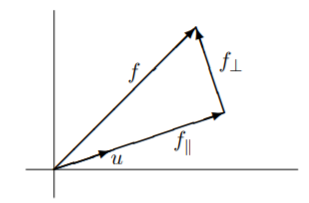
\includegraphics[scale = 0.5]{synthese_projection.PNG}
        \end{minipage}
    \end{center}
    
    On vérifie alors que
    \begin{equation*}
        \langle u,f_{\bot} \rangle = \langle u,f - \langle u,f \rangle u \rangle = \langle u,f \rangle - \langle u,f \rangle \langle u,u \rangle = 0.
    \end{equation*}
    Prenons n'importe quel autre vecteur $\alpha u$ parallèle à $u$. En utilisant \ref{theo:pythagore}, on obtient alors
    \begin{equation*}
        ||f-\alpha u||^2 = ||f_\bot + (f_\sslash - \alpha u)||^2 = ||f_\bot + (\langle u,f \rangle u - \alpha u)||^2 = ||f_\bot||^2 + |\langle f,u \rangle - \alpha|^2 ||u||^2 = ||f_\bot||^2 + |\langle f,u \rangle - \alpha|^2.
    \end{equation*}
    On trouve donc que $||f-\alpha u||$ est minimal pour $\alpha = \langle f,u \rangle$.
\end{proof}

\begin{theo}[Cauchy-Schwarz]
    Soit $\mathcal{H}$ un espace vectoriel à produit scalaire. Pour tout $f,g\in\mathcal{H}$
    \begin{equation*}
        \left|\langle f,g \rangle\right| \leq ||f||\ ||g||.
    \end{equation*}
    On parle alors de norme induite. (il y a égalité si $f$ et $g$ sont parallèles).
    \label{theo:Cauchy-Schwarz}
\end{theo}

\begin{proof}
    Commençons par le cas le plus trivial où $g=0$. On a alors $\left|\langle f,g \rangle\right| = ||f||\ ||g|| = 0$ et la proposition est vérifiée. Supposons maintenant que $g$ soit non nul et définissons le vecteur unitaire $u$ par
    \begin{equation*}
        u := \frac{g}{||g||}.
    \end{equation*}
    On cherhce alors à montrer que
    \begin{equation*}
        \left|\langle f,u \rangle\right| \leq ||f||
    \end{equation*}
    ce qui est correct puisque
    \begin{equation*}
        ||f||^2 = ||f_\sslash||^2 + ||f_\bot||^2 = \left|\langle f,u \rangle\right|^2 + ||f_\bot||^2.
    \end{equation*}
\end{proof}

Le théorème de Cauchy-Schwarz a pour conséquence que
\begin{itemize}
    \item $\mathcal{H}\times\mathcal{H}\to\mathbb{R}:f,g\to\langle f,g \rangle$ est continue ;
    \item $||\cdot|| = \sqrt{\langle\cdot,\cdot\rangle}$ satisfait bien l'inégalité du triangle.
\end{itemize}

\begin{theo}[Jordan-von Neumann]
    Soit $||\cdot||$ une norme. Il existe alors un produit scalaire $\langle\cdot,\cdot\rangle$ tel que $||\cdot|| = \sqrt{\langle\cdot,\cdot\rangle}$ ssi $\forall f,g$ :
    \begin{equation*}
        ||f+g||^2 + ||f-g||^2 = 2||f||^2 + 2||g||^2 \quad\mathrm{(r\Grave{e}gle\ du\ parall\Acute{e}logramme)}
    \end{equation*}
    Dans ce cas, on peut retrouver le produit scalaire par la définition de la norme :
    \begin{equation*}
        \langle f,g \rangle = \frac{||f+g||^2 - ||f-g||^2}{4}
    \end{equation*}
\end{theo}

Rappelons que notre but initial était d'obtenir un produit scalaire sur $C(I)$. On peut définir un tel produit sur $I=[a,b]$ par
\begin{equation*}
    \langle f,g \rangle := \int_a^b f(x)g(x)\ dx
\end{equation*}
La relation vérifie les 3 propriétés du produit scalaire.

\begin{definition}
    $\mathcal{L}_{cont}^2(I)$ est un espace préhilbertien : c'est l'ensemble $C(I)$ muni du produit scalaire définit ci-dessus.
\end{definition}

\begin{remark}
    Les ensembles $\mathcal{L}_{cont}^2(I)$ et $C(I)$ ne diffèrent que par la norme qui leur est attribué. En effet, à $\mathcal{L}_{cont}^2(I)$ on associe la norme induite alors qu'à $C(I)$ est associé la norme infinie.
\end{remark}

\begin{definition}
    On définit par $||f||_2$ la norme de $f$ dans $\mathcal{L}_{cont}^2(I)$ :
    \begin{equation*}
        ||f||_2 = \sqrt{\int_a^b |f(x)|^2 dx} \neq ||f||_\infty.
    \end{equation*}
\end{definition}

\begin{definition}
    $||\cdot||_n$ est \textbf{plus forte} que $||\cdot||_m$ si $\exists p>0$ tel que $||\cdot||_m\leq p||\cdot||_n$
\end{definition}

$\bigg($ Propriétés :
\begin{enumerate}[label=(\roman*)]
    \item Si $||\cdot||_m \leq p||\cdot||_n$, toutes suites de Cauchy définies avec $||\cdot||_n$ en est aussi une avec$||\cdot||_m$
    \item Si $F:X \rightarrow Y$ est continue dans $(X,||\cdot||_m)$, elle l'est aussi dans $(X,||\cdot||_n)$
    \item Si un ensemble est dense dans $(X,||\cdot||_n)$, il l'est aussi dans $(X,||\cdot||_m)$. $\bigg)$
\end{enumerate}

\begin{remark}
    $||f||_2\leq\sqrt{b-a}||f||_\infty$, c'est-à-dire que $||\cdot||_\infty$ est plus fort que $||\cdot||_2$.
\end{remark}

\begin{theo}
    $\mathcal{L}_{cont}^2(I)$ est séparable.
\end{theo}
\begin{proof}
    $C(I),\ ||\cdot||_\infty$ est séparable, c'est-à-dire qu'il contient un sous-ensemble dense et dénombrable. Ce sous-ensemble est dense dans $\mathcal{L}_{cont}^2(I)$ vu la remarque précédente. Il reste donc séparable avec cette nouvelle norme.
\end{proof}

\begin{theo}
    $\mathcal{L}_{cont}^2(I)$ n'est pas complet. Ce n'est donc pas un espace de Hilbert.
\end{theo}
\begin{proof}
    Soit $I=[0,2]$. On définit : 
    \begin{center}
        \begin{minipage}{0.2\textwidth}
            \begin{tikzpicture}
                \draw[<->] (0,1) |- (1.5,0);
                \draw[red] (0,0) -- (.65,0) -- (1,.75) -- (1.5,.75);
                \draw[blue] (0,0) -- (.3,0) -- (1,.75) -- (1.5,.75);
            \end{tikzpicture}
        \end{minipage}
        \begin{minipage}{0.5\textwidth}
            \begin{equation*}
                f_n(x) = \left\{\begin{array}{ll}
                    0 & \forall x \leq 1 - \frac{1}{n}\\
                    1 & \forall x > 1\\
                    \end{array}\right.
            \end{equation*}
        \end{minipage}
    \end{center}
    Donc $(f_n)_{n=1}^\infty$ est une suite de Cauchy car $||f_n - f_m||_2 \underset{m,n\to\infty}{\longrightarrow} 0$, mais ne converge vers rien car convergerait de manière discontinue :
    \begin{center}\begin{tikzpicture}
        \draw[<->] (0,1) |- (1.5,0);
        \draw[red] (0,0) -- (.75,0) node[] {\small{$\bullet$}};
        \draw[red] (.75,.75) node[]{\small{$\circ$}} -- (1.5,.75);
        \draw[red,dashed] (.75,0) -- (.75,.75);
    \end{tikzpicture}\end{center}
    Pour qu'effectivement, il existe une fonction $f$ respectant la relation ci-dessus, il faut que $f(x) = 0$ si $x<1$, 1 si $x>1$ et que $f\in C(I)$, ce qui est impossible. On conclut que l'espace des fonctions est donc incomplet.
\end{proof}

Pour espérer pouvoir rendre cet espace complet, on ne peut ni modifier la norme, ni le produit scalaire. On va alors ajouter une (ou plusieurs) propriété(s) (on va élargir l'espace) :
\begin{description}
    \item[Essai 1] $\mathcal{R}(I) = \{ f:I\to\mathbb{R} | f \ \mathrm{int\Acute{e}grable\ au\ sens\ de\ Riemannn,\ avec}\ \langle\cdot,\cdot\rangle \mathrm{ci-dessus} \} \ \cdots$ ECHEC :
        \begin{itemize}
            \item \textbf{Soucis 1 :} La norme induite $||f||_2$ est une semi-norme (pas une norme)
            \item \textbf{Soucis 2 :} $R(I)$ n'est pas complet...
        \end{itemize}
    \item[Essai 2] $C(I)\cup\{ (f_n)_{n=1}^\infty \big| (f_n)_{n=1}^\infty \subset C(I),\ \mathrm{sont\ de\ Cauchy\ et\ divergent\ pour}\ ||\cdot||_2\}$ (divergent signifie qu'il n'existe pas de fonction dans $C(I)$ qui soit de Cauchy). Le problème de cette propriété est que la fonction $||\cdot||$ serait alors une semi-norme.
    \item[Essai 3] $\mathcal{L}^2(I) = C(I)\cup\big\{ \{ (\Tilde{f}_n)_{n=1}^\infty\subset C(I)\big| ||\Tilde{f}_n-f_n||_2\to0 \}\bigg| (f_n)_{n=1}^\infty\subset C(I),\ \mathrm{Cauchy\ et\ divergente\ pour}\ ||\cdot||_2 \big\}$. Cet espace défini comme étant \textbf{la complétion} de $C(I)$ pour $||\cdot||_2$. On gardera cette définition là, malgré le fait qu'elle soit pas très pratique.
\end{description}


\subsection{Notion de convergence}

\begin{definition}
    Soit $X$ un espace muni d'une distance $d$ sur lequel est défini une suite de fonctions $(f_n)$ à valeurs réelles ou complexes. Si $\forall \epsilon > 0,\ \exists N\in\mathbb{N}$ tel que $\forall n\geq N,\ d(f_n,f)<\epsilon$, alors $f_n$ converge vers $f$ pour $n$ tendant vers l'infini.
\end{definition}

\begin{definition}
    Soit $X$ un espace vectoriel muni d'une norme $||\cdot||$ sur lequel est défini une suite de fonctions $(f_n)$ à valeurs réelles ou complexes. Si $\forall \epsilon > 0,\ \exists N\in\mathbb{N}$ tel que $\forall n\geq N,\ ||f_n - f||<\epsilon$, alors $f_n$ converge vers $f$ pour $n$ tendant vers l'infini.
\end{definition}

\begin{definition}
    Soit $X$ un espace vectoriel muni d'un produit scalaire $\langle\cdot,\cdot\rangle$ ($||\cdot|| = \sqrt{\langle\cdot,\cdot\rangle}$) sur lequel est défini une suite de fonctions $(f_n)$ à valeurs réelles ou complexes. Si $\forall \epsilon > 0,\ \exists N\in\mathbb{N}$ tel que $\forall n\geq N,\ \langle f_n,f \rangle <\epsilon$, alors $f_n$ converge vers $f$ pour $n$ tendant vers l'infini.
\end{definition}

\begin{definition}
    Soit $X$ un espace vectoriel muni d'une topologie $\mathcal{O}$ sur lequel est défini une suite de fonctions $(f_n)$ à valeurs réelles ou complexes. Cette suite de fonctions converge vers $f$ pour $n$ tendant vers l'infini f si $\forall \ \text{ouvert}\ O \ni f,\ \exists N\in\mathbb{N}$ tel que $\forall n\geq N,\ f_n \in O$.
\end{definition}


\subsection{Opérateurs linéaires}
% Section 2.3

\begin{definition}
    La relation linéaire $A$ entre les deux espaces normés $X$ et $Y$ est appelé \textbf{opérateur linéaire}
    \begin{equation*}
        A:\mathcal{D}(A)\subseteq X\rightarrow Y \qquad X,Y\ \mathrm{des\ espaces\ vectoriels}\ ||\cdot||^2.
    \end{equation*}
    si $\forall x_0,x_1 \in \mathcal{D}(A), \lambda_0,\lambda_1 \in \mathbb{C}$ : $\lambda_0x_0 + \lambda_1x_1 \in \mathcal{D}(A)$ et $A(\lambda_0x_0 + \lambda_1x_1) = \lambda_0A(x_0) + \lambda_1A(x_1)$.\\
    
    Le sous-espace linéaire $\mathcal{D}(A)$ sur lequel $A$ est défini est appelé \textbf{domaine} de $A$ et requiert fréquemment d'être dense. Le \textbf{noyau} (ou <<\textbf{null space}>>)
    \begin{equation*}
        \mathrm{Ker}(A) := \left\{ f\in\mathcal{D}(A)|Af = 0 \right\} \subseteq X \qquad (\text{= sous-espace vectoriel fermé})
    \end{equation*}
    et l'espace colonne
    \begin{equation*}
        \mathrm{Ran}(A) := \left\{ Af|f\in\mathcal{D}(A) \right\} = A\mathcal{D}(A) \subseteq Y
    \end{equation*}
    sont définis comme d'habitude.
\end{definition}

\begin{definition}
    L'opérateur $A$ est \textbf{borné} si
    \begin{equation*}
        ||A|| := \sup_{\scriptsize{\begin{array}{c}f\in\mathcal{D}(A) \\ ||f||_X=1\end{array}}} ||Af||_Y = \sup_{\scriptsize{\begin{array}{c}f\in\mathcal{D}(A) \\ ||f||_X\neq0\end{array}}} \frac{||Af||_Y}{||f||_X} < \infty.
    \end{equation*}
\end{definition}

\begin{theo}
    Un opérateur linéaire $A$ est borné si et seulement s'il est continu.
\end{theo}
\begin{proof}
    \begin{description}
        \item[borné $\Rightarrow$ continu] Borné $\Rightarrow\ ||Af||_Y \leq ||A||\ ||f||_X$ pour tout $f\in\mathcal{D}(A)$. On a donc que $A$ est de Lipschitz de constante $||A||$, et donc que $A$ est continu.
        \item[continu $\Rightarrow$ borné] Supposons que $A$ est continu et non borné. Alors il existe une suite $(u_n)_{n=1}^\infty$ de vecteur unitaire ($||u_n||_X=1$) telle que $||Au_n||_Y\geq n$. Alors $f_n := \frac{1}{n}u_n$ converge vers 0 mais pas $Af_n$ puisque $||Af_n||_Y \geq 1$. Si $A$ n'est pas borné, il n'est pas continu. On conclut donc que si $A$ est continu, alors il est borné.
    \end{description}
\end{proof}

\begin{theo}
    Soit $A:\mathcal{D}(A) \subset X \rightarrow Y $ un opérateur linéaire. Toutes les propriétés suivantes sont équivalentes :
    \begin{itemize}
        \item $A$ est borné
        \item l'image de $\mathcal{D}(A) \cap \overline{B_1}(0)$ est bornée
        \item l'image de tout sous-ensemble borné de $\mathcal{D}(A)$ est bornée
        \item $A$ est continu en $0$
        \item $A$ est continu sur $\mathcal{D}(A)$
        \item $A$ est Lipschitzien ($||Af-Ag||_Y \leq k ||f-g||_X \ \forall f,g \in \mathcal{D}(A),k\geq0$).
    \end{itemize}
\end{theo}

\begin{theo}
    Si $X$ est de dimension finie, alors tout opérateur est borné (et donc continu).
\end{theo}

\begin{proof}
    Soit $\{x_j\}_{j=1}^n$ une base de $X$. Tout vecteur $x \in X$ peut dès lors s'écrire $x=\sum \limits_{j=1}^n \alpha_jx_j$. Prenons sans pertes de généralité que $||x||_X = \sqrt{\sum \limits_{j=1}^n |a_j|^2}$ (dans un espace de dimension finie, toutes les normes sont équivalentes). Alors,
    \begin{equation*}
        ||Ax||_Y = ||A\sum \limits_{j=1}^n \alpha_jx_j||_Y \leq \sum_{j=1}^n |\alpha_j|||Ax_j||_Y \leq \sqrt{ \sum_{j=1}^n ||Ax_j||_Y^2}||x||_X
    \end{equation*}
    Donc $||A|| \leq \sqrt{\sum \limits_{j=1}^n ||Ax_j||_Y^2}$
\end{proof}

\begin{example}
    Soit $X=l^p(\mathbb{N})$ et $a\in l^\infty(\mathbb{N})$. Considérons l'opérateur multiplication $A:X\rightarrow Y$ défini par
    \begin{equation*}
        (Ab)_j := a_jb_j \ \forall b \in X.
    \end{equation*}
    Alors, $|(Ab)_j| \leq ||a||_\infty |b_j|$ montre que $||A||\leq||a||_\infty$. En réalité, on a même que $||A||=||a||_\infty$
\end{example}

\begin{example}
    Pour $X=l^p(\mathbb{N})$, on définit $A:X\rightarrow Y$ pour $f \in X$ par $(Af)_j = f_{j+1}$. Dès lors, on peut prouver que $||A|| = 1$. Le même résltat est obtenu pour l'application définie par $(Af)_1 = 0$ et $(Af)_j = f_{j-1}$.
\end{example}

\begin{example}
    Considérons l'espace vectoriel des fonctions différentiables $X=C^1[0,1]$ et équipons-le d'une norme
    \begin{equation*}
        ||f||_{\infty,1} := \max_{x\in[0,1]}|f(x)| + \max_{x\in[0,1]}|f'(x)|.
    \end{equation*}
    Soit $Y=C[0,1]$ muni de la norme $||\cdot||_\infty$. Nous observons que l'opérateur différentiel $A = \frac{d}{dx} : X\rightarrow Y$ (Soit $f \in C^1[0,1]$, $Af = f'\in C[0,1]$) est borné car
    \begin{equation*}
        ||Af||_Y = \max_{x\in[0,1]} |f'(x)| \leq \max_{x\in[0,1]} |f(x)| + \max_{x\in[0,1]} |f'(x)| = ||f||_{\infty,1} = ||f||_X.
    \end{equation*}
    Cependant, si nous considérons que $A=\frac{d}{dx}:\mathcal{D}(A)\subseteq Y\rightarrow Y$ défini sur $\mathcal{D}(A) = C^1[0,1]$, alors nous avons un opérateur non borné. Pour le montrer, choisissons
    \begin{equation*}
        u_n = \sin(n\pi x)
    \end{equation*}
    qui est normalisé par $||u_n||_\infty = 1$ et observons que
    \begin{equation*}
        Au_n(x) = u'_n(x) = n\pi\cos(n\pi x)
    \end{equation*}
    est non borné, $||Au_n||_\infty = n\pi$.
\end{example}

\begin{example}
    Soit $X=C[0,1]$. On définit $A:X \rightarrow X$ par $(Af)(x)=\int_0^xf(t)\ dt$. L'opérateur $A$ est borné et $||A||=1$ : $|\int_0^x f(t)\ dt| \leq x||f||_\infty$ et $||Af||_X = ||\int_0^x f(t)\ dt||_X$.
\end{example}

\begin{remark}
    Lorsqu'on prend la même norme dans les espaces de départ et d'arrivée, l'opérateur de dérivation n'est pas borné alors que celui d'intégration l'est! Cela provient du fait que l'intégration a une propriété de positivité de l'intégrale d'un fonction positive que la dérivée n'a pas.
\end{remark}

\begin{theo}
    Soit $A:\mathcal{D}(A)\subset X\to Y$ un opérateur linéaire et borné. Si $\mathcal{D}(A)$ est dense dans $X$ et que $Y$ est un espace de Banach (normé complet), il existe alors une seule extension continue $\overline{A}:\overline{\mathcal{D}(A)} \subset X \rightarrow Y$ linéaire et bornée telle que $||\overline{A}|| = ||A||$ et $\overline{A}\big|_{\mathcal{D}(A)} = A$ ($\overline{A}\big|_{\mathcal{D}(A)}$ = $\overline{A}$ restreint au domaine $\mathcal{D}(A)$).
\end{theo}
\begin{proof}
    \begin{description}
        \item[\textbf{Définition de $\overline{A}$ :}] Nous recherchons $\overline{A}f$ tel que $(f_n)_{n=1}^\infty\subset\mathcal{D}(A) \to f \in \overline{\mathcal{D}(A)}$ qui existe car $\mathcal{D}(A)$ est dense dans $X$. Comme $Y$ est complet, on peut poser $\overline{A}f = \lim_{n\to\infty}Af_n$, qui existe car $(f_n)$ converge et est donc une suite de Cauchy, donc $(Af_n)$ est également de Cauchy et converge.
        
        Montrons que $\overline{A}f$ est indépendant de la suite $f_n$ choisie : soit $(g_n)\subset\mathcal{D}(A)$ tel que $g_n \to f$. On a
        \begin{align*}
            ||Af_n - Ag_n||_Y & = ||A(f_n - g_n)||_Y \\
            & \leq ||A||\ ||f_n - g_n||_X \to 0 \\
            \Rightarrow \lim \limits_{n\to \infty}||\overline{A}f - Ag_n||_Y & = \lim \limits_{n\to \infty}||Af_n - Ag_n||_Y = 0.
        \end{align*}
        On conclut alors que $Ag_n\to\overline{A}f$.
        \item[\textbf{Restriction :}] $\overline{A}$ est bien une extension de $A$ car si on choisit $f \in \mathcal{D}(A)$ tel que $f_n = f$, on a $\overline{A}f = \lim \limits_{n \to\infty} Af = Af$.
        \item[\textbf{$\overline{A}$ est linéaire :}]
        \begin{align*}
            \overline{A}(\alpha f + \beta g) & = \lim_{n\to\infty} A(\alpha f_n + \beta g_n) \\ & = \lim_{n\to\infty} (\alpha A f_n + \beta A g_n) \\
            & = \alpha\overline{A} f + \beta\overline{A} g.
        \end{align*}
        \item[\textbf{Borne :}] Montrons que $||\overline{A}|| = ||A||$ :
        \begin{align*}
            ||\overline{A}|| & = \sup_{||f||_X=1} ||\overline{A}f||_Y \\ & = \sup_{||f||_X=1} ||\lim_{n\to\infty}Af_n||_Y \\
            & = \sup_{||f||_X=1} \lim_{n\to\infty}||Af_n||_Y \\ & \leq \sup_{||f||_X=1} \lim_{n\to\infty}||A||\ ||f_n||_X \\
            & = \sup_{||f||_X=1}||A|| \underbrace{\lim_{n\to\infty} ||f_n||_X}_{||f||_X} \\
            & = ||A||
        \end{align*}
    \end{description}
\end{proof}

\begin{definition}
    On représente par $\mathcal{L}(X,Y)$ l'ensemble des opérateurs linéaires bornés de $X$ dans $Y$ : $\mathcal{L}(X,Y) = \{A:X \to Y | A$ est linéaire et bornée$\}$ . On admet les deux énoncés suivant :
    \begin{itemize}
        \item $\mathcal{L}(X) := \mathcal{L}(X,X)$ et
        \item $X^\star := \mathcal{L}(X,\mathbb{C})$ est l'ensemble \textbf{dual} de $X$. Les éléments de $X^\star$ sont appelés \textbf{fonctionnelles linéaires bornés}.
    \end{itemize}
\end{definition}

\begin{example}
    Soit l'espace $X=l^p(\mathbb{N})$. On définit $l_j(a) := a_j$. On a alors $l_j\in X^\star$. On cherche alors $||l_j||$.
    \begin{equation*}
        \left.\begin{array}{rcl}
            |l_j(a)| = |a_j| \leq \big[\sum \limits_{j\in\mathbb{N}} |a_j|^p\big]^\frac{1}{p} = ||a||_p & \Rightarrow & ||l_j|| \leq 1 \\
            |l_j(\delta^j)| = 1 & \Rightarrow & ||l_j|| \geq 1
        \end{array}\right\} ||l_j|| = 1.
    \end{equation*}
\end{example}

\begin{example}
    Soit l'espace $X=C[0,1]$ avec la norme $||\cdot||_\infty$. Soit $f\in X$. On définit l'opérateur $l$ par $lf := f(1)$. Alors $l\in X^\star$ car $|lf|=|f(1)|\leq \sup \limits_{[0,1]}|f| = ||f||_\infty$. En fait, $||l|| = 1$.
    
    $l \not\in \mathcal{L}^2_{cont}[0,1]^\star$ : si $f_n(x) = \sqrt{n}x^{\frac{n-1}{2}}$, on a $||f_n||_2 = \sqrt{\int_0^1|f_n(x)|^2 \ dx} = \sqrt{\int_0^1 nx^{n-1} \ dx} = [x^n]_0^1=1$ mais $|lf_n| = \sqrt{n}\to \infty$.
\end{example}

\begin{theo}
    $\mathcal{L}(X,Y)$ avec la norme d'opérateur est un espace vectoriel normé, et de Banach si $Y$ est de Banach.
\end{theo}

\begin{example}
    $X = C[0,1],\ ||\cdot||_\infty$. Soit $g$ et $f_n$ intégrables sur $[0,1]$. On a
    \begin{equation*}
        l_g(f) := \int_0^1 g(x)f(x)\ dx.
    \end{equation*}
    Alors $l_g\in X^\star$ avec $||l_g|| = \int_0^1 |g(x)|dx =: ||g||_1$ :
    \begin{itemize}
        \item $|l_gf| = |\int_0^1 f(x)g(x) \ dx| \leq \int_0^1|f(x)|\ |g(x)| \ dx \leq ||f||_\infty \int_0^1|g(x)| \ dx \implies ||l_g||\leq\int_0^1|g(x)|\ dx$
        \item Soit $\epsilon>0$. On pose $f_\epsilon=\frac{g^*}{|g|+\epsilon}$ ($g^*$ = conjugué de g).Dès lors, $||f_\epsilon||_\infty = \sup\limits_{[0,1]} \frac{|g|}{|g|+\epsilon}\leq1$
        
        $||l_g|| \geq |l_gf_\epsilon| = \int_0^1\frac{|g(x)|^2}{|g(x)|+\epsilon}\ dx \geq \int_0^1 \frac{|g(x)|^2-\epsilon^2}{|g(x)|+\epsilon}\ dx \geq \int_0^1 |g(x)|-\epsilon\ dx = \int_0^1 |g(x)| \ dx - \epsilon$.
    \end{itemize}
\end{example}



%partie 2 : voir syntheses prof
\section{Espaces de Hilbert}
\sectionmark{Espaces de Hilbert}


\subsection{Bases orthonormées}
% Sous-section 3.1

\begin{definition}
    Un ensemble $\{u_j\}_{j\in\mathcal{J}}\subset\mathcal{H}$ est un ensemble orthonormé si $\langle u_j,u_k \rangle = \delta_{jk}$. L'ensemble d'indice $\mathcal{J}$ peut être un ensemble fini ou non, dénombrable ou non.
    
    Un ensemble orthonormé est formé de vecteurs linéairments indépendants.
\end{definition}
\begin{proof}
    Considérons un vecteur $a = \sum \limits_{l=1}^m \alpha_lu_{j_l} = 0$. Le produit scalaire de $a$ avec $u_{j_n}$ donne : $\langle a,u_{j_n} \rangle = \langle \sum \limits_{l=1}^m \alpha_lu_{j_l}, u_{j_n} \rangle = \sum \limits_{l=1}^m \alpha_l \langle u_{j_l},u_{j_n} \rangle = \alpha_n = 0$. Si nous effectuons cette opération pour différents $n$, nous observons que $a = 0$ ssi $\alpha_l = 0 \ \forall l$.
\end{proof}

\begin{lemme}
\label{lemme:Bessel}
    Soit $\{u_j\}_{j=1}^n$ un ensemble orthonormé fini et $f\in\mathcal{H}$. Alors
    \begin{equation*}
        \left\{ \begin{array}{rcll}
            f & = & f_\bot + f_\sslash  \\
            f_\sslash & = & \sum_{j} \alpha_j u_j & \mathrm{c\Grave{a}d}\ f_\sslash\in\setSpan\{u_j\}_{j=1}^n \\
            f_\bot & \bot & u_{j,\sslash} & \mathrm{c\Grave{a}d}\ \langle u_j,f_\bot \rangle = 0\ \forall j
        \end{array} \right.
    \end{equation*}
    a une et une seule solution donnée par
    \begin{equation*}
        f_\sslash = \sum_{j=1}^n \langle u_j,f \rangle u_j.
    \end{equation*}
    On a alors $||f||^2 = \sum_{j=1}^n \big|\langle u_j,f \rangle\big|^2 + ||f_\bot||^2$.
    
    $f_\sslash$ est la projection de $f$ sur $\setSpan\{ u_1,u_2,\cdots,u_n \}$. Soit $\hat{f}= \sum \limits_{j=1}^n\alpha_ju_j$. Dès lors,
    \begin{align*}
        ||f-\hat{f}||^2 &= ||f_\sslash + f_\bot -\hat{f}||^2 \\
        &= ||f_\bot||^2 + ||\sum \limits_{j=1}^n \big( \langle u_j,f\rangle - \alpha_j\big)u_j||^2\\
        &= ||f_\bot||^2 + \sum \limits_{j=1}^n|\langle u_j,f\rangle -\alpha_j|^2
    \end{align*}
    Donc, $||f-\hat{f}||^2 \geq ||f_\bot||^2$ et $||f-\hat{f}||^2$ est minimal pour $\alpha_j=\langle u_j,f \rangle$.
\end{lemme}

\begin{theo}[Inégalité de Bessel]
    \begin{equation*}
        ||f||^2 \geq \sum_{j=1}^n \big|\langle u_j,f \rangle\big|^2
    \end{equation*}
\end{theo}

On peut maintenant généraliser dans le cas où $\{u_j\}$ est de dimension infinie. Définissons tout d'abord la notion de \textbf{somme infinie}.

\begin{definition}
    Considérons une famille de nombres positifs $\{a_j\}_{j\in\mathcal{J}}$. La somme est définie par
    \begin{equation*}
        \sum_{j\in\mathcal{J}} a_j = \sup\left\{\sum_{j\in K} a_j\big| K\subseteq \mathcal{J} < \infty\right\}
    \end{equation*}
    Dès lors, on a $\sum_{j\in\mathcal{J}} a_j \geq \sum_{j\in K} a_j$.
\end{definition}

Soit $\{u_j\}_{j\in\mathcal{J}}$ un ensemble orthonormé dans $\mathcal{H}$, si $K\subseteq\mathcal{J}<\infty$, on a par l'inégalité de Bessel : 
\begin{equation*}
    \sum\limits_{j\in K}|\langle u_j,f\rangle|^2 \leq ||f||^2.
\end{equation*}
Dès lors, 
\begin{equation*}
    \sum\limits_{j\in \mathcal{J}}|\langle u_j,f\rangle|^2 = \sup\left\{\sum_{j\in K} |\langle u_j,f\rangle|^2 \big| K\subseteq \mathcal{J} < \infty\right\} \leq ||f||^2
\end{equation*}

Par définition de suprémum, $\exists (K_n)_{n\in\mathbb{N}}\subset \mathcal{J}$ tels que
\begin{equation*}
    \lim_{n\to\infty} \sum_{j\in K_n} |\langle u_j,f\rangle|^2 = \sum_{j\in\mathcal{J}} |\langle u_j,f\rangle|^2
\end{equation*}

Prenons maintenant, $K_m,K_n \subset \mathcal{J} < \infty$ et posons $f_n = \sum_{j\in K_n} \langle u_j,f\rangle u_j \in \mathcal{H}$.
\begin{align*}
    ||f_n-f_m||^2 & = ||\sum_{j\in K_n} \langle u_j,f\rangle u_j - \sum_{j\in K_m} \langle u_j,f\rangle u_j||^2\\
    & = \left\langle \sum_{j\in K_n} \langle u_j,f\rangle u_j - \sum_{j\in K_m} \langle u_j,f\rangle u_j , \sum_{j\in K_n} \langle u_j,f\rangle u_j - \sum_{j\in K_m} \langle u_j,f\rangle u_j\right\rangle\\
    & = \left\langle \sum_{j\in K_n} \langle u_j,f\rangle u_j,\sum_{j\in K_n} \langle u_j,f\rangle u_j\right\rangle + \left\langle \sum_{j\in K_m} \langle u_j,f\rangle u_j ,  \sum_{j\in K_m} \langle u_j,f\rangle u_j \right\rangle\\
    & - 2\left\langle \sum_{j\in K_n} \langle u_j,f\rangle u_j ,  \sum_{j\in K_m} \langle u_j,f\rangle u_j \right\rangle\\
    & = \Big[\sum_{j\in K_n} \langle u_j,f\rangle\Big]^2 \langle u_j,u_j\rangle + \Big[\sum_{j\in K_m} \langle u_j,f\rangle\Big]^2 \langle u_j,u_j\rangle - 2 \Big[\sum_{j\in K_n} \langle u_j,f\rangle\Big]^2 \langle u_j,u_j\rangle\\
    & = \sum_{j\in K_n} |\langle u_j,f\rangle|^2 + \sum_{j\in K_m} |\langle u_j,f\rangle|^2 - 2 \sum_{j\in (K_n \cap K_m)} |\langle u_j,f\rangle|^2\\
    & = -\sum_{j\in K_n} |\langle u_j,f\rangle|^2 - \sum_{j\in K_m} |\langle u_j,f\rangle|^2 + 2 \sum_{j\in (K_n \cup K_m)} |\langle u_j,f\rangle|^2\\
    & \leq  -\sum_{j\in K_n} |\langle u_j,f\rangle|^2 - \sum_{j\in K_m} |\langle u_j,f\rangle|^2 + 2 \sum_{j\in \mathcal{J}} |\langle u_j,f\rangle|^2
\end{align*}

En faisant tendre $n,m$ vers l'infini, on trouve que $||f_n-f_m||^2 \to 0$. De plus, si $\mathcal{H}$ est un ensemble complet, on sait que la suite $f_n$ converge vers $\sum \limits_{j\in\mathcal{J}} \langle u_j,f\rangle u_j$.

Considérons une autre suite $(\widetilde{K}_n)_{n\in\mathbb{N}}$ avec $\widetilde{f}_n = \sum_{j\in \widetilde{K}_n} \langle u_j,f\rangle u_j$. On trouve que $\sum_{j\in \mathcal{J}} \langle u_j,f\rangle u_j$ est indépendant du choix de la suite d'ensembles finis :
\begin{equation*}
    ||f_n - \widetilde{f}_n||^2 \leq  -\sum_{j\in K_n} |\langle u_j,f\rangle|^2 - \sum_{j\in \widetilde{K}_n} |\langle u_j,f\rangle|^2 + 2 \sum_{j\in \mathcal{J}} |\langle u_j,f\rangle|^2 \to 0
\end{equation*}

On peut maintenant généraliser le lemme \ref{lemme:Bessel} en dimension infinie : tout $f \in \mathcal{H}$ peut s'écrire sous la forme $f=f_\sslash + f_\bot$ avec $\langle f_\sslash,f_\bot \rangle = 0$ et $f_\sslash = \sum\limits_{j\in\mathcal{J}} \langle u_j,f\rangle u_j$. De plus, $\langle u_j,f_\bot\rangle = 0$ et $||f||^2 =\sum\limits_{j\in\mathcal{J}} |\langle u_j,f\rangle|^2+||f_\bot||^2$.

Ensuite, $\forall \hat{f} \in \overline{\text{span}(\{u_j\})}$ (adhérence des combilis de $\{u_j\}$), $||f-\hat{f}||^2\geq||f_\bot||^2$ avec égalité ssi $f_\sslash=\hat{f}$.

\begin{definition}
    Un ensemble orthonormé $\{u_j\}_{j\in\mathcal{J}}$ est une \textbf{base orthonormée} de l'espace $\mathcal{H}$ si $\forall f\in\mathcal{H}$
    \begin{equation*}
        f = \sum_{j\in\mathcal{J}} \langle u_j,f \rangle u_j
    \end{equation*}
\end{definition}

\begin{example}
    Les vecteur de la suite $(\delta^n_j)_{j\in\mathbb{N}}$ tels que $\delta^n_j=1$ ssi $n=j$ forment une base de $l^2(\mathbb{N})$
\end{example}
\begin{proof}
    Prenons un vecteur $a\in l^2(\mathbb{N})$. Dès lors, on a que $\sum \limits_{j=1}^n \langle \delta^j,a\rangle\delta^j$ donne les $n$ premières composantes du vecteur $a$. Donc, $||\sum \limits_{j=1}^n \langle \delta^j,a\rangle\delta^j-a||^2 = \sum \limits_{j=n+1}^\infty |a_j|^2$. Or on sait que $||a||_2$ est finie donc le dernier élément de $a$ tend vers $0$ ce qui permet de conclure : $||\sum \limits_{j=1}^n \langle \delta^j,a\rangle\delta^j-a||^2 \underset{n\to\infty}{\longrightarrow}0$.
\end{proof}

\begin{theo}[Gram-Schmidt]
    Tout espace de Hilbert séparable a une base orthonormée dénombrable.
\end{theo}
\begin{proof}
    Par définition de séparabilité, il existe un ensemble $\{f_n\}$ dénombrable et dense dans $\mathcal{H}$. On va procéder de manière récursive afin de trouver une base.
    
    Tout d'abord, retirons de l'ensemble $\{f_n\}$ les éléments $f_n$ qui sont une combinaison linéaire des éléments $f_1,...,f_{n-1}$. Ensuite, on pose $\widetilde{f}_n = f_n-\sum_{j=1}^{n-1}\langle u_j,f\rangle u_j \neq 0$ par indépendance linéaire. Le nouvel élément de la base doit être normalisé et vaut donc $u_n = \frac{\widetilde{f}_n}{||\widetilde{f}_n||}$.
    
    On a donc le procédé de Gram-Schmidt : $\{u_j\}_{j=1}^\infty$ défini récursivement par
    \begin{equation*}
        u_n = \frac{f_n - \sum_{j=1}^{n-1} \langle u_j,f \rangle u_j}{\left|\left|f_n - \sum_{j=1}^{n-1} \langle u_j,f \rangle u_j \right|\right|}
    \end{equation*}
    
    Si $\text{dim}\mathcal{H}<\infty$, $\{f_n\}$ est un ensemble fini et $\{u_n\}$ est une base au sens algébrique.
\end{proof}

\begin{example}
    Considèrons $\mathcal{L}^2_{cont}[-1,1]$ muni du produit scalaire $\langle f,g \rangle = \int_{-1}^1 f^*(x)g(x) \ dx$. Étant donné que les polynômes sont denses dans cet ensemble, on peut trouver une base orthonormée en partant de $f_n(x)=x^n$ pour $n\in\mathbb{N}$ :
    \begin{table}[H]
        \centering
        \begin{tabular}{ll}
            $\widetilde{f}_0(x) = 1$ & $u_0(x)=\frac{1}{\sqrt{\int_{-1}^1 1 \ dx}} = \sqrt{\frac{1}{2}}$ \\
            $\widetilde{f}_1(x) = x-\frac{1}{\sqrt{2}}\int_{-1}^1 \frac{x}{\sqrt{2}} \ dx = x$ & $u_1(x)=\frac{x}{\sqrt{\int_{-1}^1 x^2 \ dx}} = \sqrt{\frac{3}{2}}x$ \\
            $\widetilde{f}_2(x) = x^2-\frac{1}{\sqrt{2}}\int_{-1}^1 \frac{x^2}{\sqrt{2}} \ dx - \sqrt{\frac{3}{2}}x\int_{-1}^1 \sqrt{\frac{3}{2}}x^3 \ dx = x^2 - \frac{1}{3}$ & $u_2(x)=\frac{x^2 - \frac{1}{3}}{\sqrt{\int_{-1}^1 \big(x^2 - \frac{1}{3}\big)^2 \ dx}} = \sqrt{\frac{5}{2}}\frac{3x^2-1}{2}$ \\
        \end{tabular}
    \end{table}
    Les polynômes obtenus sont appelés les polynômes de Legendre.
\end{example}

\begin{theo}
    Pour un ensemble orthonormé $\{ u_j \}_{j\in\mathcal{J}}$ de $\mathcal{H}$, les conditions suivantes sont équivalentes :
    \begin{enumerate}[label=(\roman*)]
        \item $\{ u_j \}_{j\in\mathcal{J}}$ forment un ensemble orthormé maximal (on ne peut pas ajouter un vecteur à l'ensemble tout en gardant un ensemble orthonormé);
        \item $\{ u_j \}_{j\in\mathcal{J}}$ forment une base orthonormée, c'est-à-dire que pour tout $f\in\mathcal{H}$, $f = \sum_{j\in\mathcal{J}} \langle u_j,f \rangle u_j$
        \item $\forall f\in\mathcal{H}$ : $||f||^2 = \sum_{j\in\mathcal{J}} \big| \langle u_j,f \rangle \big|^2$ (relation de Parseval) ;
        \item $\{f\in\mathcal{H}\big|\forall j\in\mathcal{J}, \ \langle u_j,f \rangle = 0\} = \{0\}$.
    \end{enumerate} \label{theo:ens_ortho}
\end{theo}
\begin{proof}
    Puisque les éléments de $\{ u_j \}_{j\in\mathcal{J}}$ sont orthormaux entre eux, on a pour tout $f\in\mathcal{H}$ que
    \begin{enumerate}[label=(\alph*)]
        \item $f = \sum_{j\in\mathcal{J}} \langle u_j,f \rangle u_j + f_\bot$ où $f_\bot$ est perpendiculaire à $u_j$ pour tout $j$ ;
        \item $||f||^2 = \sum_{j\in\mathcal{J}} \big|\langle u_j,f \rangle\big|^2 + ||f_\bot||^2$
        \item $||f-f_\sslash|| \leq \left|\left| f - \sum_{j\in\mathcal{J}}\alpha_j u_j \right|\right|$ pour tout $\alpha_j\in\mathbb{R}$.
    \end{enumerate}
    \begin{description}
        \item[\textit{(i)$\Rightarrow$(ii)}] Si non-\textit{(ii)}, il existe un vecteur perpendiculaire à tous les autres, notamment $f_\bot = f-\sum_{j\in\mathcal{J}}\langle u_j, f\rangle u_j \neq 0$, qu'on peut normaliser et ajouter à la base et $\{u_j\}_{j\in\mathcal{J}} \cup \{\frac{f_\bot}{||f_\bot||}\ $ serait un ensemble orthonormé (non-\textit{(i)}).
        \item[\textit{(ii)$\Rightarrow$(iii)}] Si \textit{(ii)}, alors $f_\bot = 0$ dans (a), de même que dans (b), donc \textit{(iii)}.
        \item[\textit{(iii)$\Rightarrow$(iv)}] Si \textit{(iii)} et $\langle u_j,f \rangle = 0$ $\forall j\in\mathcal{J}$, alors $||f||^2 = 0$, donc $f=0$.
        \item[\textit{(iv)$\Rightarrow$(i)}] Si non-\textit{(i)}, donc si $\{u_j\}$ n'est pas maximal, on peut trouver $\{u_j\}\cup\{g\}$ qui serait orthonormé. Or $g\in \mathcal{H}$ et donc des hypothèses de \textit{(iv)} on en conclut que $\langle u_j,g\rangle = 0 \implies g = 0$.
    \end{description}
\end{proof}

\iffalse
\begin{definition}
    Un opérateur $U\in\mathcal{L(\mathcal{H}_1,\mathcal{H}_2)}$ est \textbf{unitaire} s'il est bijectif et que
    \begin{equation}
        \langle U_g,U_f \rangle_2 = \langle g,f \rangle_1 \quad \forall g,f \in \mathcal{H}_1.
    \end{equation}
    Dans ce cas, on dit que $\mathcal{H}_1$ et $\mathcal{H}_2$ sont \textbf{unitairement équivalents}.
\end{definition}

\begin{theo}
    Tout espace de Hilbert séparable de dimension infinie est unitairement équivalent à $l^2(\mathbb{N})$.
\end{theo}
\begin{proof}
    Soit $\{u_j\}_{j\in\mathbb{N}}$ une base orthormale de $\mathcal{H}$. Montrons que $U:\mathcal{H}\to l^2(\mathbb{N}) : f\mapsto(\langle u_j,f \rangle)_{j\in\mathbb{N}}$ est unitaire.
    \begin{itemize}
        \item[$\bullet$] Il préserve la norme au vu du théorème \ref{theo:ens_ortho} ;
        \item[$\bullet$] Il est injectif
        \item[$\bullet$] Il est surjectif car pour tout $a\in l^2(\mathbb{N})$, $f:=\sum_{j\in\mathbb{N}} a_j u_j$ est bien défini et $U_f=a$.
    \end{itemize}
\end{proof}

\begin{theo}
    Tout espace de Hilbert admet une base orthonormale.
\end{theo}

\fi

\subsection{Projection de Riesz}
% Sous-section 3.2
\begin{theo}[Projection]
    Si $M \subset \mathcal{H}$ est un sous espace vectoriel fermé de $\mathcal{H}$, il existe un opérateur $P_M \in \mathcal{L}(\mathcal{H},\mathcal{H})$ tel que $\forall f\in\mathcal{H}$, $P_Mf \in M$ et $\forall f \in \mathcal{H},g\in M$, $\langle f-P_Mf,g\rangle=0$.
    
    En particulier, $\forall g\in M$, $||P_Mf-f||\leq||g-f||$ et $\forall f \in M$, $P_Mf = f$.
\end{theo}
\begin{proof}
    Comme $M$ est un sous-espace FERMÉ de Hilbert, il est lui même un espace de Hilbert. Posons $P_Mf = \sum_{j\in\mathcal{J}} \langle u_j,f\rangle u_j$ où $\{u_j\}$ est une base orthonormée de $M$ (l'opérateur $P_M$ renvoie $f_\sslash$). L'espace $M$ doit être fermé car $M=\{f\in\mathcal{H}\big|f=P_Mf\}$.
    
    Si on pose $M^\bot = \{f\big|\langle g,f\rangle=0 \ \forall g\in M\}$, on obtient $P_{M^\bot}f=f - P_Mf \implies P_{M^\bot} + P_M = I$
    
    $P_M$ est appelé \textbf{projection orthogonal} de $M$. 
\end{proof}

\begin{lemme}[Riesz]
    Si $\mathcal{H}$ est un espace de Hilbert, alors, pour toute fonctionnelle linéaire $l\in\mathcal{H}^\star=\mathcal{L}(\mathcal{H},\mathbb{C})$, il existe un vecteur $g\in\mathcal{H}$ tel que $\forall f\in\mathcal{H}$, on ait $l(f)=\langle f,g\rangle$.
\end{lemme}
\begin{proof}
    \begin{itemize}
        \item Si $l=0$, $l(f)=0 \ \forall f \in \mathcal{H}$ et $g=0$;
        \item Sinon, on a $\text{Ker}(l)=\{f\big|l(f)=0\}\subset \mathcal{H}$. On prend alors $\widetilde{g}\in\text{Ker}(l)^\bot$ tel que $||\widetilde{g}||=1$. On pose $g = l(\widetilde{g})^*\widetilde{g}$. Dès lors, $ \forall f\in\mathcal{H}$,
        \begin{equation*}
            l(f) = l(\widetilde{g})\langle \widetilde{g},f\rangle+\langle\widetilde{g},l(f)\widetilde{g}-l(\widetilde{g})f\rangle = l(\widetilde{g})\langle\widetilde{g},f\rangle=\langle g,f\rangle
        \end{equation*}
        car $l(l(f)\widetilde{g}-l(\widetilde{g})f)=l(f)l(\widetilde{g})-l(\widetilde{g})l(f)=0$.
    \end{itemize}
\end{proof}

\subsection{Séries de Fourier}
% Sous-section 3.3

\begin{definition}
    Soit $f:[-\pi,\pi]\to\mathbb{C}$ une fonction intégrable. Sa \textbf{série de Fourier} s'écrit
    \begin{equation*}
        S(f)(x) = \frac{a_0}{2} + \sum_{k\in\mathbb{N}}[a_k\cos(kx)+b_k\sin(kx)] = \sum_{k\in\mathbb{Z}}\hat{f}_ke^{ikx}
    \end{equation*}
    avec les coeeficients de Fouriers suivants
    \begin{align*}
        a_k & = \frac{1}{\pi}\int_{-\pi}^\pi \cos(kx)f(x) \ dx\\
        b_k & = \frac{1}{\pi}\int_{-\pi}^\pi \sin(kx)f(x) \ dx\\
        \hat{f}_k & = \frac{1}{2\pi}\int_{-\pi}^\pi e^{-iky}f(y) \ dy
    \end{align*}
\end{definition}

\begin{definition}
    Cette série peut s'écrire à l'aide du \textbf{noyau de Dirichlet} :
    \begin{equation*}
        S_n(f)(x) = \sum_{k=-n}^n\hat{f}_ke^{ikx} = \frac{1}{2\pi}\int_{-\pi}^\pi D_n(x-y)f(y)dy
    \end{equation*}
    avec
    \begin{equation*}
        D_n(x) = \sum_{k=-n}^n e^{ikx} = \frac{e^{i(n+1)x}-e^{-inx}}{e^{ix}-1} = \frac{e^{i(n+\frac{1}{2})x}-e^{-i(n+\frac{1}{2})x}}{e^{\frac{ix}{2}}-e^{\frac{-ix}{2}}} = \frac{\sin[(n+\frac{1}{2})x]}{\sin[\frac{x}{2}]}
    \end{equation*}
    Cette fonction satisfait les propriétés suivantes :
    \begin{itemize}
        \item $D_n(-x)=D_n(x)=D_n(x+2\pi)$
        \item $|D_n(x)|_{max} = D_n(0)=2n+1$
        \item $\int_{-\pi}^\pi D_n(x)\ dx = \sum\limits_{k=-n}^n \int_{-\pi}^\pi e^{ikx}\ dx = \sum_{k=-n}^n \frac{2\sin(k\pi)}{k} = 2\pi$ (tout s'annule sauf en $k=0$ où on obtient $\frac{0}{0}$ et en faisant l'hospital on obtient $\frac{2\pi\cos(k\pi)}{1}=2\pi$)
    \end{itemize}
\end{definition}

\begin{theo}
    Si on muni $ L^2[-\pi,\pi]$ (espace de Lebesgue :  fonctions telles que $f^p$ est intégrable au sens de Lebesgue) du produit scalire $\langle f,g\rangle = \frac{1}{2\pi}\int_{-\pi}^\pi f^*g$, les fonctions $\{e^{ikx}\}_{k\in\mathbb{N}}$ forment un ensemble orhtonormé. En effet,
    \begin{equation*}
        \int_{-\pi}^\pi e^{-ikx}e^{ilx} \ dx = \int_{-\pi}^\pi e^{ix (l-k)} \ dx = \Bigg[\frac{e^{ix(l-k)}}{i(l-k)}\Bigg]_{-\pi}^\pi = 2\pi\delta_{l,k}
    \end{equation*}
    donc $\langle e^{ikx},e^{ilx}\rangle = \delta_{k,l}$.
    
    De plus, cet ensemble est une base de $ L^2[-\pi,\pi]$ donc :
    \begin{itemize}
        \item $\{e^{ikx}\}_{k\in\mathbb{Z}}$ est un ensemble orthonormé maximal de $ L^2[-\pi,\pi]$
        \item $\forall f\in L^2[-\pi,\pi],\ \lim\limits_{n\to\infty}||S_n(f)-f||=0$ (convergence ponctuelle)
        \item $\forall f\in L^2[-\pi,\pi],\ \sum\limits_{k\in\mathbb{Z}}|\hat{f}_k|^2=\frac{1}{2\pi}\int_{-\pi}^\pi |f(x)|^2\ dx$
        \item si $f\in L^2[-\pi,\pi]$ et $\int_{-\pi}^\pi e^{ikx}f(x)\ dx = 0$ pour tout $k\in\mathbb{N}$, alors $f=0$.
    \end{itemize}
\end{theo}

Mais si $f$ est une fonction continue, la suite $(S_nf)$ ne converge pas toujours vers $f$ (de manière uniforme)... On va donc s'intéresser à la moyenne de la série de Fourier.

\begin{definition}
    On définit les \textbf{sommes de Fourier moyennées} par
    \begin{equation*}
        \overline{S}_n(f)(x)=\frac{1}{n}\sum_{k=0}^{n-1}S_k(f) = \frac{1}{2\pi}\int_{-\pi}^\pi F_n(x-y)f(y)\ dy
    \end{equation*}
    où $F_n$ est le \textbf{noyau de Fejér} :
    \begin{align*}
        F_n(x) &= \frac{1}{n} \sum_{k=0}^{n-1}D_k(x)
        = \frac{1}{2in\sin\big(\frac{x}{2}\big)}\sum_{k=0}^{n-1}e^{i(k+\frac{1}{2})x}-e^{-i(k+\frac{1}{2})x}\\
        & = \frac{1}{2in\sin\big(\frac{x}{2}\big)} \Bigg(\frac{e^{i(n+\frac{1}{2})x}-e^{\frac{ix}{2}}}{e^{ix}-1}-\frac{e^{-i(n+\frac{1}{2})x}-e^{\frac{ix}{2}}}{e^{-ix}-1}\Bigg)\\
        & = \frac{e^{inx}-2+e^{-inx}}{2in\sin\big(\frac{x}{2}\big)(e^{\frac{ix}{2}}-e^{\frac{-ix}{2}}} = \frac{\big(e^{\frac{inx}{2}}-e^{\frac{-inx}{2}}\big)^2}{2in\sin\big(\frac{x}{2}\big)(e^{\frac{ix}{2}}-e^{\frac{-ix}{2}}}
        = \frac{1}{n}\Bigg(\frac{\sin\big(\frac{nx}{2}\big)}{\sin\big(\frac{x}{2}\big)}\Bigg)^2
    \end{align*}
    Cette fonction satisfait les propriétés suivantes :
    \begin{itemize}
        \item $F_n(-x)=F_n(x)=F_n(x+2\pi)\geq0$
        \item $\int_{-\pi}^\pi F_n(x)\ dx = 2\pi$
    \end{itemize}
\end{definition}

\begin{theo}[Fejer]
    Soit $f:\mathbb{R}\to\mathbb{C}$ une fonction continue et périodique de période $2\pi$, alors $\overline{S}_n(f)\to f$ uniformément.
\end{theo}
\begin{proof}
    Par périodicité de $F_n$ et $f$ :
    \begin{equation*}
        \overline{S}_n(f)(x) = \frac{1}{2\pi}\int_{-\pi}^\pi F_n(x-y)f(y)\ dy = \frac{1}{2\pi}\int_{-\pi}^\pi F_n(z)f(x-z)\ dz
    \end{equation*}
    \begin{equation*}
        \overline{S}_n(f)(x)-f(x) = \frac{1}{2\pi}\int_{-\pi}^\pi F_n(z)[f(x-z)-f(x)]\ dz
    \end{equation*}
    On peut en déduire que $\forall \delta>0$ :
    \begin{align*}
        |\overline{S}_n(f)(x)-f(x)| & = \frac{1}{2\pi}\int_{-\pi}^\pi F_n(z)|f(x-z)-f(x)|\ dz\\
        & = \frac{1}{2\pi}\Bigg(\int_{-\delta}^\delta F_n(z)|f(x-z)-f(x)|\ dz + \int_{-\pi}^{-\delta} F_n(z)|f(x-z)-f(x)|\ dz \\
        & + \int_{\delta}^\pi F_n(z)|f(x-z)-f(x)|\ dz\Bigg)\\
        & \leq \sup\limits_{z\in[-\delta,\delta]}|f(x-z)-f(x)|+\frac{2||f||_\infty}{n\sin\big(\frac{\delta}{2}\big)^2}
    \end{align*}
    car $\int_{-\delta}^\delta F_n(z)\ dz\leq 2\pi$, $F_n(x)\leq\frac{1}{n\sin\big(\frac{\delta}{2}\big)^2}\ \forall \delta\leq|x|\leq\pi$ et $|f(x-z)-f(x)| \leq 2||f||_\infty$ (et $\pi-\delta\leq\pi$).
    
    Comme $f$ est uniformément continue, si on prend $\delta$ suffisamment petit, le premier terme va valoir $0$. On choisit ensuite $n$ suffisamment grand afin de rendre le second terme faible. On trouve donc que $\overline{S}_n(f)$ converge uniformément vers $f$.
\end{proof}

On peut utiliser ce résultat afin de démontrer que $S_n(f)\to f$ dans $ L^2[-\pi,\pi] \ \forall f\in L^2[-\pi,\pi]$.
\begin{proof}
    En effet,
\end{proof}
%partie 2 : voir syntheses prof
%\part{Analyse réelle}

\section{Les mesures}
% Section 5

\begin{theo}
    Soit $f$ une fonction continue sur l'intervalle $[a,b]$. Alors $f$ est intégrable sur cette intervalle selon Riemann.
\end{theo}

\begin{definition}
    La mesure de Lebesgue sur $\mathbb{R}$ est notée $\lambda$. Si $a<b$ et $u\in\mathcal{C}([a,b])$, alors $u$ est intégrable par rapport à $\lambda$ sur $[a,b]$ et
    \begin{equation}
        \int_{[a,b]}u(x)\ d\lambda(x) = \int_a^b u(x)\ dx,
    \end{equation}
    où $\int_a^b u(x)\ dx$ est l'intégrale de Riemann de $u$ sur $[a,b]$.
\end{definition}

\begin{definition}
    Soit $\Omega$ un ensemble, $\mu$ une mesure sur $\Omega$ et $u:\Omega\rightarrow\mathbb{R}$ une fonction mesurable positive. Par définition, pour toute partie mesurable $A$ de $\Omega$,
    \begin{equation*}
        \int_A u\ d\mu = \int_\Omega u\chi_A\ d\mu,
    \end{equation*}
    où
    \begin{equation}
        \chi_A = \left\{\begin{array}{ll}
            1 & \mathrm{si}\ x\in A, \\
            0 & \mathrm{si}\ x\in\Omega\setminus A.
        \end{array}\right.
    \end{equation}
\end{definition}

\begin{theo}[Lebesgue]
    \begin{equation}
        f\ \mathrm{est\ int\Acute{e}grable} \quad\Leftrightarrow\quad \mu_{\mathrm{Lebesgue}}(\{\mathrm{discontinu\ de}\ f\}) = 0.
    \end{equation}
\end{theo}

\begin{definition}[Intégrale de Lebesgue]
    \begin{equation}
        \int f(x) d\mu(x) := \int_0^\infty f^{-1}(t) dt
    \end{equation}
\end{definition}

\noindent
On voudrait au moins que $\mu$ satisfasse :
\begin{enumerate}
    \item $\mu([a,b]) = b-a \rightarrow \int_a^b 1d\mu = b-a$ ;
    \item $\mu(\biguplus_{n=1}^\infty A_n) = \sum_{n=1}^\infty \mu(A_n)$ ;
    \item $A\subseteq B \Rightarrow \mu(A)\leq\mu(B)$ ;
    \item $\mu(A+B) = \mu(A)$ (pour $A+B := \{a+b|a\in A\}$) ;
    \item $\mu(x)\ \exists\ \forall x\ \mathrm{born\Acute{e}}\subset\mathbb{R}$ ;
    \item $\mu(\mathbb{Q}\cap[0,1]) = 0 \Rightarrow \int_0^1 \chi_\mathbb{Q}(x) d\mu = 0 \Leftarrow$ 1. et 2.
\end{enumerate}
Ceci est cependant impossible car les points 1. et 5. ne sont pas compatibles. On peut construire un ``ensemble de Vitali'' $E\subset[0,1]$ tel que $[0,1]\subset\biguplus_{q\in\mathbb{Q}\cap[-1,1]}(E+q)\subset [-1,2]$ :
\begin{equation*}
    \underbrace{\mu([0,1])}_{=1} \leq \sum_{n=1}^\infty \underbrace{\mu(E+q_n)}_{=\mu(E)} \leq \underbrace{\mu([-1,2])}_{=3}
\end{equation*}
Or, si $\mu(E)\to0$, nous avons que $1\nleq0\leq3$ et si $\mu(E)>0$ $1\leq \sum_n \mu(E)\to\infty\nleq3$. On doit alors renoncer à une propriété pour rendre la démarche possible et l'on accepte finalement le fait que l'on ne puisse pas tout mesurer. On se restreint aux ensembles qui sont Lebesgue mesurables.

\begin{definition}
    $A\subseteq\mathbb{R}$ est \textbf{Lebesgue mesurable} si $\forall E\subset\mathbb{R}$.
    \begin{equation}
        \lambda^\star(E) = \lambda^\star(A\cap E) + \lambda^\star(A'\cap E).
    \end{equation}
\end{definition}

\begin{remark}
    La collection des sous-ensembles Leb-mesurables forme une $\sigma$-algèbre et $\lambda^\star$ restreinte à cette $\sigma$-algèbre est une mesure appelée \textbf{mesure de Lebesgue}.
\end{remark}

\subsection{$\sigma$-algèbre et mesures}

\begin{definition}
    Une $\sigma$-algèbre est une famille $\Sigma$ de sous-ensemble d'un ensemble donné $X$ telle que
    \begin{enumerate}[label=(\roman*)]
        \item $X\in\Sigma$ ;
        \item $\Sigma$ est stable par union dénombrables ;
        \item $\Sigma$ est stable par passage au complémentaire.
    \end{enumerate}
\end{definition}

\begin{example}
    La collection des $A\subseteq\mathbb{R}$ est Lebesgue-mesurable (à admettre). Si $X$ un espace topologiue et $\Sigma =: B(X)$ est la plus petite $\sigma$-algèbre qui contient les ouvert de $X$, on dit alors qu'elle est la \textbf{$\sigma$-algèbre borélienne} de X et ses éléments sont les \textbf{ensembles boréliens}.
\end{example}

\begin{definition}
    $(X,\Sigma)$ où $\Sigma$ est $\sigma$-algèbre de $X$ est un \textbf{espace mesurable}. Les éléments de $\Sigma$ sont les \textbf{ensembles mesurables}.
\end{definition}

\begin{definition}
    Une mesure $\mu$ est une \textbf{fonction} $\mu : \Sigma\to[0,\infty)$ telle que
    \begin{enumerate}[label=(\roman*)]
        \item $\mu(\emptyset)=0$ ;
        \item $\mu(\biguplus_{n=1}^\infty A_n) = \sum_{n=1}^\infty \mu(A_n)$, $A_n\in\Sigma$ ($\sigma$-additivité).
    \end{enumerate}
\end{definition}

\begin{definition}
    La mesure $\mu$ est dite \textbf{finie} si $\mu(X)<\infty$ et représente une \textbf{mesure probalistique} si $\mu(X)=1$. Elle est dit \textbf{$\sigma$-finie} s'il y a un nombre dénombrable de couvertures $\{X_n\}_{n=1}^\infty$ de $X$ telles que $X_n\in\Sigma$ et $\mu(X)<\infty$ pour tout $n$. Tous les ensembles de $\Sigma$ sont appelés \textbf{ensembles mesurables} et le triplet $(X,\Sigma,\mu)$ fait référence à un \textbf{espace mesurable}.
\end{definition}

\begin{theo}
    Tout espace borélien est Lebesgue-mesurable (par définition de l'espace borélien).
\end{theo}

\begin{theo}
    Toute mesure $\mu$ satisfait
    \begin{enumerate}[label=(\roman*)]
        \item $A\subseteq B \Rightarrow \mu(A)\leq\mu(B)$
        \item $A_n\nearrow A (\Leftrightarrow A_n \subseteq A_{n+1}, \bigcup_{n=1}^\infty A_n = A) \Rightarrow  \mu(A_n) \underset{n\to\infty}{\to} \mu(A)$
        \item $A_n \searrow A, \mu(A_n)<\infty \Rightarrow \mu(A_n) \underset{n\to\infty}{\to} \mu(A)$
    \end{enumerate}
\end{theo}
\begin{proof}
    \begin{enumerate}[label=(\roman*)]
        \item $\mu(B) = \mu(A) + \mu(B\setminus A)$
        \item Définissons $\tilde{A}_1 = A_1, \tilde{A}_n = A_n\setminus A_{n-1}$ et remarquons que chacun des ces espaces sont disjoints et satisfont la relation $A_n = \bigcup_{j=1}^n \tilde{A}_j$. Dès lors, nous avons que
        \begin{equation*}
            \mu(A_n) = \sum_{j=1}^n \mu(\tilde{A}_j) \to \sum_{j=1}^\infty \mu(\tilde{A}_j) = \mu(\bigcup_{j=1}^\infty \tilde{A}_j) = \mu(A)
        \end{equation*}
        par $\sigma$-additivité.
        \item En utilisant, à l'inverse du cas précédent, $\tilde{A}_n = A_1\setminus A_n \nearrow A_1\setminus A$, ce qui implique que
        \begin{equation*}
            \mu(\tilde{A}_n) = \mu(A_1) - \mu(A_n) \to \mu(A_1\setminus A) = \mu(A_1) - \mu(A).
        \end{equation*}
    \end{enumerate}
\end{proof}

\subsection{Mesures de Borel}

\begin{definition}
    Une propriété est vraie \textbf{$\mu$-presque partout} si elle est vraie dans le complémentaire d'un ensemble de mesure nulle.
\end{definition}

\begin{example}
    $\lambda(Q) = 0$ donc $\chi_Q = 0$ $\lambda$-presque partout.
\end{example}

\begin{example}[Ensemble de Cantor]
    \begin{figure}[H]
        \centering
        \begin{tikzpicture}
            \draw[|-|] (0,0) node[below]{$\small{0}$} -- (9,0) node[below]{$\small{1}$};
            \draw[|-|] (0,-1) node[below]{$\small{0}$} -- (3,-1) node[below]{$\small{\nicefrac{1}{3}}$};
            \draw[|-|] (6,-1) node[below]{$\small{\nicefrac{2}{3}}$} -- (9,-1) node[below]{$\small{1}$};
            \draw[|-|] (0,-2) node[below]{$\small{0}$} -- (1,-2) node[below]{$\small{\nicefrac{1}{9}}$};
            \draw[|-|] (2,-2) node[below]{$\small{\nicefrac{2}{9}}$} -- (3,-2) node[below]{$\small{\nicefrac{3}{9}}$};
            %\draw[|-|] (4,-2) node[below]{$\small{\nicefrac{4}{9}}$} -- (5,-2) node[below]{$\small{\nicefrac{5}{9}}$};
            \draw[|-|] (6,-2) node[below]{$\small{\nicefrac{6}{9}}$} -- (7,-2) node[below]{$\small{\nicefrac{7}{9}}$};
            \draw[|-|] (8,-2) node[below]{$\small{\nicefrac{8}{9}}$} -- (9,-2) node[below]{$\small{1}$};
            \draw (-1,0) node[]{$\small{C_0}$};\draw (-1,-1) node[]{$\small{C_1}$};\draw (-1,-2) node[]{$\small{C_2}$};
        \end{tikzpicture}
    \end{figure}
    On se demande si l'ensemble $C := \bigcap_{n=0}^\infty C_n$ est Lebesgue-mesurable. Oui, il l'est puisque $C$ est défini comme étant l'intersection d'ensembles fermés, donc $C$ est borélien et donc Lebesgue-mesurable. Plus précisément, dès lors que $C_n$ est compact, on peut dire que $C$ l'est aussi. De plus, $C_n$ est formé de $2^n$ intervalles de longueur $3^{-n}$, et la mesure de Lebesgue associée est alors $\lambda(C_n) = \left(\frac{2}{3}\right)^n$. En particulier, $\lambda(C) = \lim_{n\to\infty} \lambda(C_n) = 0$. \textit{On en conclut alors que tout ensemble $A$ dénombrable a une mesure de Lebesgue nulle ; la réciproque n'est pas vraie, par contre, puisque $C$ n'est pas dénombrable} (on peut en effet écrire $C$ en base ternaire).
\end{example}

\begin{definition}[Mesure de Lebesgue-Stieltjes]
    On se restreint au cas où $X=\mathbb{R}$. Commençons par un ensemble simple, avant de généraliser pour chaque ensemble de Borel. Or, à chaque mesure de Borel sur $\mathfrak{B}$, on peut assigner une fonction de distribution :
    \begin{equation}
        \mu(x) := \left\{ \begin{array}{ll}
            -\mu((x,0]), & x<0 \\
            0, & x=0 \\
            \mu([0,x)), & x>0
        \end{array} \right.
    \end{equation}
    qui est continue et non décroissante.
\end{definition}

\subsection{Fonctions mesurables}

\begin{definition}
    Soit $(X,\Sigma_X)$ et $(Y,\Sigma_Y)$ des espaces mesurables. Alors $f:X\to Y$ est \textbf{mesurable} si $f^{-1}(A)\in\Sigma_X$ $\forall A\in\Sigma_Y$.
\end{definition}

\begin{lemme}
    Pour $Y=\mathbb{R}^n$ et $\Sigma_Y = \mathcal{B}(\mathbb{R}^n)$, $f:X\to\mathbb{R}^n$ est mesurable ssi $f^{-1}((a,\infty))\in\Sigma_X$ $\forall A\in\mathbb{R}^n$
\end{lemme}

\begin{prop}
    Si $f,g,f_n$ mesurables, alors il en est de même pour $(f\circ g), (f+g), (fg), \inf f_n, \sup f_n, \lim_n \inf f_n$ et $\lim_n \sup f_n$.
\end{prop}


\section{L'intégration}
% Section 6

\subsection{Une histoire de sommes}

Si $f:\mathbb{R}\to\mathbb{R}^+$ est Lebesgue mesurable, alors
\begin{equation}
    \int f d\lambda := \int_0^\infty \lambda(\{x|f(x)\geq t\}) dt
\end{equation}
où $\lambda$ est la mesure de Lebesgue, telle que
\begin{equation}
    f^\star : f \mapsto \lambda(\{x|f(x)\geq t\}).
\end{equation}
L'ensemble $\{x|f(x)\geq t\}$ est en effet Lebesgue-mesurable puisque est équivalent à $f^{-1}([t,\infty))$.

\begin{figure}[H]
    \centering
    \begin{tikzpicture}[line cap=round,line join=round,>=triangle 45,x=1cm,y=1cm]
\begin{axis}[
x=2cm,y=2cm,
axis lines=middle,
xmin=-0.4,
xmax=4.639739030061704,
ymin=-0.4,
ymax=2.8171179395620385,
xtick={0,1,...,4},
ytick={0,1,...,2},]
%\clip(-0.5151507307634132,-0.90759599412651) rectangle (6.639739030061704,3.8171179395620385);
\fill[line width=2pt,color=ffqqtt,fill=ffqqtt,pattern=dots,pattern color=ffqqtt] (1.5131875573813442,0.5005941909798874) -- (3.54,0.49883719696068573) -- (3.5390671112374505,0) -- (1.5125750909542865,0) -- cycle;
\fill[line width=2pt,color=ffqqtt,fill=ffqqtt,pattern=dots,pattern color=ffqqtt] (2.091068964522473,1.0012900264977338) -- (3.4589923819151455,0.9998386487892081) -- (3.4586572577395205,0.4989077109898341) -- (2.0910682773673903,0.5000932403504766) -- cycle;
\fill[line width=2pt,color=ffqqtt,fill=ffqqtt,pattern=dots,pattern color=ffqqtt] (2.469199959643233,1.5028818489544997) -- (3.3434430700533335,1.5011313644198092) -- (3.338487428643057,0.9999665055103682) -- (2.4691996903455786,1.0008888267672588) -- cycle;
\fill[line width=2pt,color=zzffqq,fill=zzffqq,pattern=north east lines,pattern color=zzffqq] (1.5,0) -- (1.5,0.49387141899809883) -- (1.9997364404217024,0.4920289716788111) -- (1.9949933137943323,0) -- cycle;
\fill[line width=2pt,color=zzffqq,fill=zzffqq,pattern=north east lines,pattern color=zzffqq] (1.9949933137943323,0) -- (2,0.896361676485673) -- (2.500217260046752,0.8965252151669196) -- (2.5,0) -- cycle;
\fill[line width=2pt,color=zzffqq,fill=zzffqq,pattern=north east lines,pattern color=zzffqq] (2.5,0) -- (2.4986066894155705,1.543200123756189) -- (2.9998613465700456,1.5409395347532977) -- (3,0) -- cycle;
\fill[line width=2pt,color=zzffqq,fill=zzffqq,pattern=north east lines,pattern color=zzffqq] (3.5,0) -- (3.5005723773247612,0.7599167620933662) -- (2.9999316622980072,0.7594782671387783) -- (3,0) -- cycle;
\draw[line width=2pt,color=qqttcc] (1.1000012387350137,0.38017195942680204) -- (1.1000012387350137,0.38017195942680204);
\draw[line width=2pt,color=qqttcc] (1.1000012387350137,0.38017195942680204) -- (1.1061762321082162,0.3807154652172777);
\draw[line width=2pt,color=qqttcc] (1.1061762321082162,0.3807154652172777) -- (1.1123512254814187,0.3812932077013518);
\draw[line width=2pt,color=qqttcc] (1.1123512254814187,0.3812932077013518) -- (1.1185262188546212,0.3819053755685795);
\draw[line width=2pt,color=qqttcc] (1.1185262188546212,0.3819053755685795) -- (1.1247012122278237,0.3825521572033015);
\draw[line width=2pt,color=qqttcc] (1.1247012122278237,0.3825521572033015) -- (1.1308762056010262,0.3832337406653892);
\draw[line width=2pt,color=qqttcc] (1.1308762056010262,0.3832337406653892) -- (1.1370511989742286,0.38395031367071697);
\draw[line width=2pt,color=qqttcc] (1.1370511989742286,0.38395031367071697) -- (1.1432261923474311,0.3847020635713452);
\draw[line width=2pt,color=qqttcc] (1.1432261923474311,0.3847020635713452) -- (1.1494011857206336,0.385489177335429);
\draw[line width=2pt,color=qqttcc] (1.1494011857206336,0.385489177335429) -- (1.1555761790938361,0.38631184152683095);
\draw[line width=2pt,color=qqttcc] (1.1555761790938361,0.38631184152683095) -- (1.1617511724670386,0.38717024228445074);
\draw[line width=2pt,color=qqttcc] (1.1617511724670386,0.38717024228445074) -- (1.1679261658402411,0.38806456530125843);
\draw[line width=2pt,color=qqttcc] (1.1679261658402411,0.38806456530125843) -- (1.1741011592134436,0.3889949958030312);
\draw[line width=2pt,color=qqttcc] (1.1741011592134436,0.3889949958030312) -- (1.180276152586646,0.38996171852679206);
\draw[line width=2pt,color=qqttcc] (1.180276152586646,0.38996171852679206) -- (1.1864511459598485,0.3909649176989436);
\draw[line width=2pt,color=qqttcc] (1.1864511459598485,0.3909649176989436) -- (1.192626139333051,0.39200477701309877);
\draw[line width=2pt,color=qqttcc] (1.192626139333051,0.39200477701309877) -- (1.1988011327062535,0.39308147960759876);
\draw[line width=2pt,color=qqttcc] (1.1988011327062535,0.39308147960759876) -- (1.204976126079456,0.394195208042722);
\draw[line width=2pt,color=qqttcc] (1.204976126079456,0.394195208042722) -- (1.2111511194526585,0.39534614427757453);
\draw[line width=2pt,color=qqttcc] (1.2111511194526585,0.39534614427757453) -- (1.217326112825861,0.39653446964666017);
\draw[line width=2pt,color=qqttcc] (1.217326112825861,0.39653446964666017) -- (1.2235011061990635,0.3977603648361323);
\draw[line width=2pt,color=qqttcc] (1.2235011061990635,0.3977603648361323) -- (1.229676099572266,0.39902400985971575);
\draw[line width=2pt,color=qqttcc] (1.229676099572266,0.39902400985971575) -- (1.2358510929454684,0.4003255840342985);
\draw[line width=2pt,color=qqttcc] (1.2358510929454684,0.4003255840342985) -- (1.242026086318671,0.4016652659551929);
\draw[line width=2pt,color=qqttcc] (1.242026086318671,0.4016652659551929) -- (1.2482010796918734,0.40304323347105897);
\draw[line width=2pt,color=qqttcc] (1.2482010796918734,0.40304323347105897) -- (1.254376073065076,0.4044596636584854);
\draw[line width=2pt,color=qqttcc] (1.254376073065076,0.4044596636584854) -- (1.2605510664382784,0.40591473279623224);
\draw[line width=2pt,color=qqttcc] (1.2605510664382784,0.40591473279623224) -- (1.266726059811481,0.40740861633911773);
\draw[line width=2pt,color=qqttcc] (1.266726059811481,0.40740861633911773) -- (1.2729010531846833,0.4089414888915621);
\draw[line width=2pt,color=qqttcc] (1.2729010531846833,0.4089414888915621) -- (1.2790760465578858,0.41051352418077025);
\draw[line width=2pt,color=qqttcc] (1.2790760465578858,0.41051352418077025) -- (1.2852510399310883,0.41212489502955973);
\draw[line width=2pt,color=qqttcc] (1.2852510399310883,0.41212489502955973) -- (1.2914260333042908,0.41377577332882387);
\draw[line width=2pt,color=qqttcc] (1.2914260333042908,0.41377577332882387) -- (1.2976010266774933,0.4154663300096293);
\draw[line width=2pt,color=qqttcc] (1.2976010266774933,0.4154663300096293) -- (1.3037760200506958,0.41719673501494436);
\draw[line width=2pt,color=qqttcc] (1.3037760200506958,0.41719673501494436) -- (1.3099510134238983,0.41896715727099276);
\draw[line width=2pt,color=qqttcc] (1.3099510134238983,0.41896715727099276) -- (1.3161260067971008,0.4207777646582269);
\draw[line width=2pt,color=qqttcc] (1.3161260067971008,0.4207777646582269) -- (1.3223010001703032,0.42262872398192375);
\draw[line width=2pt,color=qqttcc] (1.3223010001703032,0.42262872398192375) -- (1.3284759935435057,0.4245202009423916);
\draw[line width=2pt,color=qqttcc] (1.3284759935435057,0.4245202009423916) -- (1.3346509869167082,0.42645236010478804);
\draw[line width=2pt,color=qqttcc] (1.3346509869167082,0.42645236010478804) -- (1.3408259802899107,0.42842536486854254);
\draw[line width=2pt,color=qqttcc] (1.3408259802899107,0.42842536486854254) -- (1.3470009736631132,0.4304393774363837);
\draw[line width=2pt,color=qqttcc] (1.3470009736631132,0.4304393774363837) -- (1.3531759670363157,0.4324945587829614);
\draw[line width=2pt,color=qqttcc] (1.3531759670363157,0.4324945587829614) -- (1.3593509604095182,0.4345910686230634);
\draw[line width=2pt,color=qqttcc] (1.3593509604095182,0.4345910686230634) -- (1.3655259537827206,0.4367290653794216);
\draw[line width=2pt,color=qqttcc] (1.3655259537827206,0.4367290653794216) -- (1.3717009471559231,0.438908706150104);
\draw[line width=2pt,color=qqttcc] (1.3717009471559231,0.438908706150104) -- (1.3778759405291256,0.4411301466754849);
\draw[line width=2pt,color=qqttcc] (1.3778759405291256,0.4411301466754849) -- (1.3840509339023281,0.4433935413047938);
\draw[line width=2pt,color=qqttcc] (1.3840509339023281,0.4433935413047938) -- (1.3902259272755306,0.44569904296223606);
\draw[line width=2pt,color=qqttcc] (1.3902259272755306,0.44569904296223606) -- (1.3964009206487331,0.4480468031126801);
\draw[line width=2pt,color=qqttcc] (1.3964009206487331,0.4480468031126801) -- (1.4025759140219356,0.45043697172690766);
\draw[line width=2pt,color=qqttcc] (1.4025759140219356,0.45043697172690766) -- (1.408750907395138,0.45286969724642456);
\draw[line width=2pt,color=qqttcc] (1.408750907395138,0.45286969724642456) -- (1.4149259007683405,0.4553451265478228);
\draw[line width=2pt,color=qqttcc] (1.4149259007683405,0.4553451265478228) -- (1.421100894141543,0.45786340490669497);
\draw[line width=2pt,color=qqttcc] (1.421100894141543,0.45786340490669497) -- (1.4272758875147455,0.46042467596108993);
\draw[line width=2pt,color=qqttcc] (1.4272758875147455,0.46042467596108993) -- (1.433450880887948,0.4630290816745126);
\draw[line width=2pt,color=qqttcc] (1.433450880887948,0.4630290816745126) -- (1.4396258742611505,0.4656767622984568);
\draw[line width=2pt,color=qqttcc] (1.4396258742611505,0.4656767622984568) -- (1.445800867634353,0.46836785633446776);
\draw[line width=2pt,color=qqttcc] (1.445800867634353,0.46836785633446776) -- (1.4519758610075555,0.47110250049573476);
\draw[line width=2pt,color=qqttcc] (1.4519758610075555,0.47110250049573476) -- (1.458150854380758,0.47388082966819844);
\draw[line width=2pt,color=qqttcc] (1.458150854380758,0.47388082966819844) -- (1.4643258477539604,0.4767029768711808);
\draw[line width=2pt,color=qqttcc] (1.4643258477539604,0.4767029768711808) -- (1.470500841127163,0.4795690732175215);
\draw[line width=2pt,color=qqttcc] (1.470500841127163,0.4795690732175215) -- (1.4766758345003654,0.48247924787322316);
\draw[line width=2pt,color=qqttcc] (1.4766758345003654,0.48247924787322316) -- (1.482850827873568,0.48543362801659495);
\draw[line width=2pt,color=qqttcc] (1.482850827873568,0.48543362801659495) -- (1.4890258212467704,0.48843233879689696);
\draw[line width=2pt,color=qqttcc] (1.4890258212467704,0.48843233879689696) -- (1.495200814619973,0.4914755032924696);
\draw[line width=2pt,color=qqttcc] (1.495200814619973,0.4914755032924696) -- (1.5013758079931753,0.49456324246835414);
\draw[line width=2pt,color=qqttcc] (1.5013758079931753,0.49456324246835414) -- (1.5075508013663778,0.4976956751333905);
\draw[line width=2pt,color=qqttcc] (1.5075508013663778,0.4976956751333905) -- (1.5137257947395803,0.5008729178967899);
\draw[line width=2pt,color=qqttcc] (1.5137257947395803,0.5008729178967899) -- (1.5199007881127828,0.5040950851241814);
\draw[line width=2pt,color=qqttcc] (1.5199007881127828,0.5040950851241814) -- (1.5260757814859853,0.5073622888931193);
\draw[line width=2pt,color=qqttcc] (1.5260757814859853,0.5073622888931193) -- (1.5322507748591878,0.510674638948051);
\draw[line width=2pt,color=qqttcc] (1.5322507748591878,0.510674638948051) -- (1.5384257682323903,0.5140322426547372);
\draw[line width=2pt,color=qqttcc] (1.5384257682323903,0.5140322426547372) -- (1.5446007616055927,0.517435204954126);
\draw[line width=2pt,color=qqttcc] (1.5446007616055927,0.517435204954126) -- (1.5507757549787952,0.5208836283156584);
\draw[line width=2pt,color=qqttcc] (1.5507757549787952,0.5208836283156584) -- (1.5569507483519977,0.5243776126900248);
\draw[line width=2pt,color=qqttcc] (1.5569507483519977,0.5243776126900248) -- (1.5631257417252002,0.5279172554613409);
\draw[line width=2pt,color=qqttcc] (1.5631257417252002,0.5279172554613409) -- (1.5693007350984027,0.531502651398758);
\draw[line width=2pt,color=qqttcc] (1.5693007350984027,0.531502651398758) -- (1.5754757284716052,0.5351338926074853);
\draw[line width=2pt,color=qqttcc] (1.5754757284716052,0.5351338926074853) -- (1.5816507218448077,0.5388110684792342);
\draw[line width=2pt,color=qqttcc] (1.5816507218448077,0.5388110684792342) -- (1.5878257152180102,0.5425342656420653);
\draw[line width=2pt,color=qqttcc] (1.5878257152180102,0.5425342656420653) -- (1.5940007085912126,0.5463035679096391);
\draw[line width=2pt,color=qqttcc] (1.5940007085912126,0.5463035679096391) -- (1.6001757019644151,0.5501190562298648);
\draw[line width=2pt,color=qqttcc] (1.6001757019644151,0.5501190562298648) -- (1.6063506953376176,0.5539808086329365);
\draw[line width=2pt,color=qqttcc] (1.6063506953376176,0.5539808086329365) -- (1.6125256887108201,0.5578889001787552);
\draw[line width=2pt,color=qqttcc] (1.6125256887108201,0.5578889001787552) -- (1.6187006820840226,0.5618434029037302);
\draw[line width=2pt,color=qqttcc] (1.6187006820840226,0.5618434029037302) -- (1.624875675457225,0.565844385766948);
\draw[line width=2pt,color=qqttcc] (1.624875675457225,0.565844385766948) -- (1.6310506688304276,0.569891914595712);
\draw[line width=2pt,color=qqttcc] (1.6310506688304276,0.569891914595712) -- (1.63722566220363,0.5739860520304392);
\draw[line width=2pt,color=qqttcc] (1.63722566220363,0.5739860520304392) -- (1.6434006555768325,0.5781268574689071);
\draw[line width=2pt,color=qqttcc] (1.6434006555768325,0.5781268574689071) -- (1.649575648950035,0.5823143870098522);
\draw[line width=2pt,color=qqttcc] (1.649575648950035,0.5823143870098522) -- (1.6557506423232375,0.586548693395905);
\draw[line width=2pt,color=qqttcc] (1.6557506423232375,0.586548693395905) -- (1.66192563569644,0.5908298259558593);
\draw[line width=2pt,color=qqttcc] (1.66192563569644,0.5908298259558593) -- (1.6681006290696425,0.5951578305462686);
\draw[line width=2pt,color=qqttcc] (1.6681006290696425,0.5951578305462686) -- (1.674275622442845,0.5995327494923628);
\draw[line width=2pt,color=qqttcc] (1.674275622442845,0.5995327494923628) -- (1.6804506158160474,0.6039546215282774);
\draw[line width=2pt,color=qqttcc] (1.6804506158160474,0.6039546215282774) -- (1.68662560918925,0.6084234817365921);
\draw[line width=2pt,color=qqttcc] (1.68662560918925,0.6084234817365921) -- (1.6928006025624524,0.6129393614871639);
\draw[line width=2pt,color=qqttcc] (1.6928006025624524,0.6129393614871639) -- (1.698975595935655,0.6175022883752603);
\draw[line width=2pt,color=qqttcc] (1.698975595935655,0.6175022883752603) -- (1.7051505893088574,0.622112286158971);
\draw[line width=2pt,color=qqttcc] (1.7051505893088574,0.622112286158971) -- (1.71132558268206,0.6267693746959058);
\draw[line width=2pt,color=qqttcc] (1.71132558268206,0.6267693746959058) -- (1.7175005760552624,0.6314735698791587);
\draw[line width=2pt,color=qqttcc] (1.7175005760552624,0.6314735698791587) -- (1.723675569428465,0.6362248835725381);
\draw[line width=2pt,color=qqttcc] (1.723675569428465,0.6362248835725381) -- (1.7298505628016673,0.6410233235450575);
\draw[line width=2pt,color=qqttcc] (1.7298505628016673,0.6410233235450575) -- (1.7360255561748698,0.6458688934046719);
\draw[line width=2pt,color=qqttcc] (1.7360255561748698,0.6458688934046719) -- (1.7422005495480723,0.6507615925312615);
\draw[line width=2pt,color=qqttcc] (1.7422005495480723,0.6507615925312615) -- (1.7483755429212748,0.6557014160088455);
\draw[line width=2pt,color=qqttcc] (1.7483755429212748,0.6557014160088455) -- (1.7545505362944773,0.6606883545570297);
\draw[line width=2pt,color=qqttcc] (1.7545505362944773,0.6606883545570297) -- (1.7607255296676798,0.6657223944616697);
\draw[line width=2pt,color=qqttcc] (1.7607255296676798,0.6657223944616697) -- (1.7669005230408823,0.6708035175047504);
\draw[line width=2pt,color=qqttcc] (1.7669005230408823,0.6708035175047504) -- (1.7730755164140847,0.675931700893468);
\draw[line width=2pt,color=qqttcc] (1.7730755164140847,0.675931700893468) -- (1.7792505097872872,0.6811069171885111);
\draw[line width=2pt,color=qqttcc] (1.7792505097872872,0.6811069171885111) -- (1.7854255031604897,0.6863291342315296);
\draw[line width=2pt,color=qqttcc] (1.7854255031604897,0.6863291342315296) -- (1.7916004965336922,0.6915983150717866);
\draw[line width=2pt,color=qqttcc] (1.7916004965336922,0.6915983150717866) -- (1.7977754899068947,0.6969144178919848);
\draw[line width=2pt,color=qqttcc] (1.7977754899068947,0.6969144178919848) -- (1.8039504832800972,0.702277395933256);
\draw[line width=2pt,color=qqttcc] (1.8039504832800972,0.702277395933256) -- (1.8101254766532997,0.70768719741931);
\draw[line width=2pt,color=qqttcc] (1.8101254766532997,0.70768719741931) -- (1.8163004700265022,0.7131437654797306);
\draw[line width=2pt,color=qqttcc] (1.8163004700265022,0.7131437654797306) -- (1.8224754633997046,0.7186470380724175);
\draw[line width=2pt,color=qqttcc] (1.8224754633997046,0.7186470380724175) -- (1.8286504567729071,0.7241969479051551);
\draw[line width=2pt,color=qqttcc] (1.8286504567729071,0.7241969479051551) -- (1.8348254501461096,0.7297934223563107);
\draw[line width=2pt,color=qqttcc] (1.8348254501461096,0.7297934223563107) -- (1.8410004435193121,0.7354363833946433);
\draw[line width=2pt,color=qqttcc] (1.8410004435193121,0.7354363833946433) -- (1.8471754368925146,0.7411257474982256);
\draw[line width=2pt,color=qqttcc] (1.8471754368925146,0.7411257474982256) -- (1.853350430265717,0.7468614255724606);
\draw[line width=2pt,color=qqttcc] (1.853350430265717,0.7468614255724606) -- (1.8595254236389196,0.7526433228671889);
\draw[line width=2pt,color=qqttcc] (1.8595254236389196,0.7526433228671889) -- (1.865700417012122,0.7584713388928799);
\draw[line width=2pt,color=qqttcc] (1.865700417012122,0.7584713388928799) -- (1.8718754103853245,0.7643453673358906);
\draw[line width=2pt,color=qqttcc] (1.8718754103853245,0.7643453673358906) -- (1.878050403758527,0.7702652959727925);
\draw[line width=2pt,color=qqttcc] (1.878050403758527,0.7702652959727925) -- (1.8842253971317295,0.7762310065837501);
\draw[line width=2pt,color=qqttcc] (1.8842253971317295,0.7762310065837501) -- (1.890400390504932,0.7822423748649463);
\draw[line width=2pt,color=qqttcc] (1.890400390504932,0.7822423748649463) -- (1.8965753838781345,0.7882992703400433);
\draw[line width=2pt,color=qqttcc] (1.8965753838781345,0.7882992703400433) -- (1.902750377251337,0.794401556270669);
\draw[line width=2pt,color=qqttcc] (1.902750377251337,0.794401556270669) -- (1.9089253706245394,0.8005490895659242);
\draw[line width=2pt,color=qqttcc] (1.9089253706245394,0.8005490895659242) -- (1.915100363997742,0.8067417206908962);
\draw[line width=2pt,color=qqttcc] (1.915100363997742,0.8067417206908962) -- (1.9212753573709444,0.8129792935741684);
\draw[line width=2pt,color=qqttcc] (1.9212753573709444,0.8129792935741684) -- (1.927450350744147,0.8192616455143258);
\draw[line width=2pt,color=qqttcc] (1.927450350744147,0.8192616455143258) -- (1.9336253441173494,0.8255886070854315);
\draw[line width=2pt,color=qqttcc] (1.9336253441173494,0.8255886070854315) -- (1.939800337490552,0.8319600020414797);
\draw[line width=2pt,color=qqttcc] (1.939800337490552,0.8319600020414797) -- (1.9459753308637544,0.8383756472198054);
\draw[line width=2pt,color=qqttcc] (1.9459753308637544,0.8383756472198054) -- (1.952150324236957,0.8448353524434438);
\draw[line width=2pt,color=qqttcc] (1.952150324236957,0.8448353524434438) -- (1.9583253176101593,0.8513389204224302);
\draw[line width=2pt,color=qqttcc] (1.9583253176101593,0.8513389204224302) -- (1.9645003109833618,0.8578861466540306);
\draw[line width=2pt,color=qqttcc] (1.9645003109833618,0.8578861466540306) -- (1.9706753043565643,0.8644768193218886);
\draw[line width=2pt,color=qqttcc] (1.9706753043565643,0.8644768193218886) -- (1.9768502977297668,0.8711107191940868);
\draw[line width=2pt,color=qqttcc] (1.9768502977297668,0.8711107191940868) -- (1.9830252911029693,0.8777876195201018);
\draw[line width=2pt,color=qqttcc] (1.9830252911029693,0.8777876195201018) -- (1.9892002844761718,0.884507285926651);
\draw[line width=2pt,color=qqttcc] (1.9892002844761718,0.884507285926651) -- (1.9953752778493743,0.8912694763124163);
\draw[line width=2pt,color=qqttcc] (1.9953752778493743,0.8912694763124163) -- (2.001550271222577,0.8980739407416338);
\draw[line width=2pt,color=qqttcc] (2.001550271222577,0.8980739407416338) -- (2.0077252645957792,0.9049204213365429);
\draw[line width=2pt,color=qqttcc] (2.0077252645957792,0.9049204213365429) -- (2.0139002579689817,0.9118086521686772);
\draw[line width=2pt,color=qqttcc] (2.0139002579689817,0.9118086521686772) -- (2.0200752513421842,0.9187383591489946);
\draw[line width=2pt,color=qqttcc] (2.0200752513421842,0.9187383591489946) -- (2.0262502447153867,0.925709259916826);
\draw[line width=2pt,color=qqttcc] (2.0262502447153867,0.925709259916826) -- (2.032425238088589,0.9327210637276408);
\draw[line width=2pt,color=qqttcc] (2.032425238088589,0.9327210637276408) -- (2.0386002314617917,0.9397734713396117);
\draw[line width=2pt,color=qqttcc] (2.0386002314617917,0.9397734713396117) -- (2.044775224834994,0.9468661748989706);
\draw[line width=2pt,color=qqttcc] (2.044775224834994,0.9468661748989706) -- (2.0509502182081966,0.9539988578241412);
\draw[line width=2pt,color=qqttcc] (2.0509502182081966,0.9539988578241412) -- (2.057125211581399,0.9611711946886401);
\draw[line width=2pt,color=qqttcc] (2.057125211581399,0.9611711946886401) -- (2.0633002049546016,0.9683828511027339);
\draw[line width=2pt,color=qqttcc] (2.0633002049546016,0.9683828511027339) -- (2.069475198327804,0.975633483593839);
\draw[line width=2pt,color=qqttcc] (2.069475198327804,0.975633483593839) -- (2.0756501917010066,0.9829227394856521);
\draw[line width=2pt,color=qqttcc] (2.0756501917010066,0.9829227394856521) -- (2.081825185074209,0.9902502567760048);
\draw[line width=2pt,color=qqttcc] (2.081825185074209,0.9902502567760048) -- (2.0880001784474116,0.9976156640134213);
\draw[line width=2pt,color=qqttcc] (2.0880001784474116,0.9976156640134213) -- (2.094175171820614,1.0050185801723738);
\draw[line width=2pt,color=qqttcc] (2.094175171820614,1.0050185801723738) -- (2.1003501651938165,1.0124586145272238);
\draw[line width=2pt,color=qqttcc] (2.1003501651938165,1.0124586145272238) -- (2.106525158567019,1.019935366524831);
\draw[line width=2pt,color=qqttcc] (2.106525158567019,1.019935366524831) -- (2.1127001519402215,1.0274484256558214);
\draw[line width=2pt,color=qqttcc] (2.1127001519402215,1.0274484256558214) -- (2.118875145313424,1.0349973713245055);
\draw[line width=2pt,color=qqttcc] (2.118875145313424,1.0349973713245055) -- (2.1250501386866265,1.042581772717424);
\draw[line width=2pt,color=qqttcc] (2.1250501386866265,1.042581772717424) -- (2.131225132059829,1.0502011886705204);
\draw[line width=2pt,color=qqttcc] (2.131225132059829,1.0502011886705204) -- (2.1374001254330315,1.0578551675349152);
\draw[line width=2pt,color=qqttcc] (2.1374001254330315,1.0578551675349152) -- (2.143575118806234,1.0655432470412806);
\draw[line width=2pt,color=qqttcc] (2.143575118806234,1.0655432470412806) -- (2.1497501121794364,1.0732649541627932);
\draw[line width=2pt,color=qqttcc] (2.1497501121794364,1.0732649541627932) -- (2.155925105552639,1.081019804976656);
\draw[line width=2pt,color=qqttcc] (2.155925105552639,1.081019804976656) -- (2.1621000989258414,1.088807304524178);
\draw[line width=2pt,color=qqttcc] (2.1621000989258414,1.088807304524178) -- (2.168275092299044,1.0966269466693892);
\draw[line width=2pt,color=qqttcc] (2.168275092299044,1.0966269466693892) -- (2.1744500856722464,1.1044782139561917);
\draw[line width=2pt,color=qqttcc] (2.1744500856722464,1.1044782139561917) -- (2.180625079045449,1.1123605774640195);
\draw[line width=2pt,color=qqttcc] (2.180625079045449,1.1123605774640195) -- (2.1868000724186513,1.120273496662001);
\draw[line width=2pt,color=qqttcc] (2.1868000724186513,1.120273496662001) -- (2.192975065791854,1.128216419261605);
\draw[line width=2pt,color=qqttcc] (2.192975065791854,1.128216419261605) -- (2.1991500591650563,1.1361887810677666);
\draw[line width=2pt,color=qqttcc] (2.1991500591650563,1.1361887810677666) -- (2.205325052538259,1.144190005828463);
\draw[line width=2pt,color=qqttcc] (2.205325052538259,1.144190005828463) -- (2.2115000459114613,1.1522195050827373);
\draw[line width=2pt,color=qqttcc] (2.2115000459114613,1.1522195050827373) -- (2.217675039284664,1.1602766780071531);
\draw[line width=2pt,color=qqttcc] (2.217675039284664,1.1602766780071531) -- (2.2238500326578663,1.1683609112606623);
\draw[line width=2pt,color=qqttcc] (2.2238500326578663,1.1683609112606623) -- (2.230025026031069,1.1764715788278721);
\draw[line width=2pt,color=qqttcc] (2.230025026031069,1.1764715788278721) -- (2.2362000194042712,1.1846080418607012);
\draw[line width=2pt,color=qqttcc] (2.2362000194042712,1.1846080418607012) -- (2.2423750127774737,1.192769648518403);
\draw[line width=2pt,color=qqttcc] (2.2423750127774737,1.192769648518403) -- (2.2485500061506762,1.200955733805947);
\draw[line width=2pt,color=qqttcc] (2.2485500061506762,1.200955733805947) -- (2.2547249995238787,1.2091656194107378);
\draw[line width=2pt,color=qqttcc] (2.2547249995238787,1.2091656194107378) -- (2.260899992897081,1.217398613537664);
\draw[line width=2pt,color=qqttcc] (2.260899992897081,1.217398613537664) -- (2.2670749862702837,1.22565401074245);
\draw[line width=2pt,color=qqttcc] (2.2670749862702837,1.22565401074245) -- (2.273249979643486,1.2339310917633072);
\draw[line width=2pt,color=qqttcc] (2.273249979643486,1.2339310917633072) -- (2.2794249730166886,1.242229123350862);
\draw[line width=2pt,color=qqttcc] (2.2794249730166886,1.242229123350862) -- (2.285599966389891,1.2505473580963437);
\draw[line width=2pt,color=qqttcc] (2.285599966389891,1.2505473580963437) -- (2.2917749597630936,1.258885034258025);
\draw[line width=2pt,color=qqttcc] (2.2917749597630936,1.258885034258025) -- (2.297949953136296,1.2672413755858831);
\draw[line width=2pt,color=qqttcc] (2.297949953136296,1.2672413755858831) -- (2.3041249465094986,1.275615591144486);
\draw[line width=2pt,color=qqttcc] (2.3041249465094986,1.275615591144486) -- (2.310299939882701,1.2840068751340672);
\draw[line width=2pt,color=qqttcc] (2.310299939882701,1.2840068751340672) -- (2.3164749332559036,1.2924144067097871);
\draw[line width=2pt,color=qqttcc] (2.3164749332559036,1.2924144067097871) -- (2.322649926629106,1.3008373497991558);
\draw[line width=2pt,color=qqttcc] (2.322649926629106,1.3008373497991558) -- (2.3288249200023085,1.3092748529176048);
\draw[line width=2pt,color=qqttcc] (2.3288249200023085,1.3092748529176048) -- (2.334999913375511,1.317726048982188);
\draw[line width=2pt,color=qqttcc] (2.334999913375511,1.317726048982188) -- (2.3411749067487135,1.3261900551233991);
\draw[line width=2pt,color=qqttcc] (2.3411749067487135,1.3261900551233991) -- (2.347349900121916,1.3346659724950802);
\draw[line width=2pt,color=qqttcc] (2.347349900121916,1.3346659724950802) -- (2.3535248934951185,1.343152886082414);
\draw[line width=2pt,color=qqttcc] (2.3535248934951185,1.343152886082414) -- (2.359699886868321,1.3516498645079737);
\draw[line width=2pt,color=qqttcc] (2.359699886868321,1.3516498645079737) -- (2.3658748802415235,1.3601559598358181);
\draw[line width=2pt,color=qqttcc] (2.3658748802415235,1.3601559598358181) -- (2.372049873614726,1.3686702073736123);
\draw[line width=2pt,color=qqttcc] (2.372049873614726,1.3686702073736123) -- (2.3782248669879284,1.3771916254727534);
\draw[line width=2pt,color=qqttcc] (2.3782248669879284,1.3771916254727534) -- (2.384399860361131,1.3857192153264894);
\draw[line width=2pt,color=qqttcc] (2.384399860361131,1.3857192153264894) -- (2.3905748537343334,1.3942519607660066);
\draw[line width=2pt,color=qqttcc] (2.3905748537343334,1.3942519607660066) -- (2.396749847107536,1.4027888280544687);
\draw[line width=2pt,color=qqttcc] (2.396749847107536,1.4027888280544687) -- (2.4029248404807384,1.4113287656789928);
\draw[line width=2pt,color=qqttcc] (2.4029248404807384,1.4113287656789928) -- (2.409099833853941,1.4198707041405367);
\draw[line width=2pt,color=qqttcc] (2.409099833853941,1.4198707041405367) -- (2.4152748272271433,1.4284135557416863);
\draw[line width=2pt,color=qqttcc] (2.4152748272271433,1.4284135557416863) -- (2.421449820600346,1.4369562143723151);
\draw[line width=2pt,color=qqttcc] (2.421449820600346,1.4369562143723151) -- (2.4276248139735483,1.4454975552931055);
\draw[line width=2pt,color=qqttcc] (2.4276248139735483,1.4454975552931055) -- (2.433799807346751,1.4540364349169068);
\draw[line width=2pt,color=qqttcc] (2.433799807346751,1.4540364349169068) -- (2.4399748007199533,1.4625716905879102);
\draw[line width=2pt,color=qqttcc] (2.4399748007199533,1.4625716905879102) -- (2.446149794093156,1.4711021403586248);
\draw[line width=2pt,color=qqttcc] (2.446149794093156,1.4711021403586248) -- (2.4523247874663583,1.4796265827646308);
\draw[line width=2pt,color=qqttcc] (2.4523247874663583,1.4796265827646308) -- (2.4584997808395607,1.4881437965970918);
\draw[line width=2pt,color=qqttcc] (2.4584997808395607,1.4881437965970918) -- (2.4646747742127632,1.4966525406730055);
\draw[line width=2pt,color=qqttcc] (2.4646747742127632,1.4966525406730055) -- (2.4708497675859657,1.5051515536031723);
\draw[line width=2pt,color=qqttcc] (2.4708497675859657,1.5051515536031723) -- (2.4770247609591682,1.5136395535578601);
\draw[line width=2pt,color=qqttcc] (2.4770247609591682,1.5136395535578601) -- (2.4831997543323707,1.522115238030147);
\draw[line width=2pt,color=qqttcc] (2.4831997543323707,1.522115238030147) -- (2.489374747705573,1.530577283596917);
\draw[line width=2pt,color=qqttcc] (2.489374747705573,1.530577283596917) -- (2.4955497410787757,1.5390243456774928);
\draw[line width=2pt,color=qqttcc] (2.4955497410787757,1.5390243456774928) -- (2.501724734451978,1.547455058289879);
\draw[line width=2pt,color=qqttcc] (2.501724734451978,1.547455058289879) -- (2.5078997278251806,1.5558680338045964);
\draw[line width=2pt,color=qqttcc] (2.5078997278251806,1.5558680338045964) -- (2.514074721198383,1.564261862696089);
\draw[line width=2pt,color=qqttcc] (2.514074721198383,1.564261862696089) -- (2.5202497145715856,1.5726351132916731);
\draw[line width=2pt,color=qqttcc] (2.5202497145715856,1.5726351132916731) -- (2.526424707944788,1.5809863315180168);
\draw[line width=2pt,color=qqttcc] (2.526424707944788,1.5809863315180168) -- (2.5325997013179906,1.5893140406451207);
\draw[line width=2pt,color=qqttcc] (2.5325997013179906,1.5893140406451207) -- (2.538774694691193,1.5976167410277784);
\draw[line width=2pt,color=qqttcc] (2.538774694691193,1.5976167410277784) -- (2.5449496880643956,1.6058929098444962);
\draw[line width=2pt,color=qqttcc] (2.5449496880643956,1.6058929098444962) -- (2.551124681437598,1.6141410008338483);
\draw[line width=2pt,color=qqttcc] (2.551124681437598,1.6141410008338483) -- (2.5572996748108005,1.6223594440282422);
\draw[line width=2pt,color=qqttcc] (2.5572996748108005,1.6223594440282422) -- (2.563474668184003,1.6305466454850754);
\draw[line width=2pt,color=qqttcc] (2.563474668184003,1.6305466454850754) -- (2.5696496615572055,1.638700987015255);
\draw[line width=2pt,color=qqttcc] (2.5696496615572055,1.638700987015255) -- (2.575824654930408,1.6468208259090606);
\draw[line width=2pt,color=qqttcc] (2.575824654930408,1.6468208259090606) -- (2.5819996483036105,1.654904494659326);
\draw[line width=2pt,color=qqttcc] (2.5819996483036105,1.654904494659326) -- (2.588174641676813,1.6629503006819113);
\draw[line width=2pt,color=qqttcc] (2.588174641676813,1.6629503006819113) -- (2.5943496350500155,1.670956526033448);
\draw[line width=2pt,color=qqttcc] (2.5943496350500155,1.670956526033448) -- (2.600524628423218,1.678921427126328);
\draw[line width=2pt,color=qqttcc] (2.600524628423218,1.678921427126328) -- (2.6066996217964204,1.6868432344409125);
\draw[line width=2pt,color=qqttcc] (2.6066996217964204,1.6868432344409125) -- (2.612874615169623,1.6947201522349373);
\draw[line width=2pt,color=qqttcc] (2.612874615169623,1.6947201522349373) -- (2.6190496085428254,1.7025503582500882);
\draw[line width=2pt,color=qqttcc] (2.6190496085428254,1.7025503582500882) -- (2.625224601916028,1.7103320034157225);
\draw[line width=2pt,color=qqttcc] (2.625224601916028,1.7103320034157225) -- (2.6313995952892304,1.7180632115497074);
\draw[line width=2pt,color=qqttcc] (2.6313995952892304,1.7180632115497074) -- (2.637574588662433,1.7257420790563573);
\draw[line width=2pt,color=qqttcc] (2.637574588662433,1.7257420790563573) -- (2.6437495820356353,1.7333666746214335);
\draw[line width=2pt,color=qqttcc] (2.6437495820356353,1.7333666746214335) -- (2.649924575408838,1.7409350389041908);
\draw[line width=2pt,color=qqttcc] (2.649924575408838,1.7409350389041908) -- (2.6560995687820403,1.7484451842264363);
\draw[line width=2pt,color=qqttcc] (2.6560995687820403,1.7484451842264363) -- (2.662274562155243,1.7558950942585773);
\draw[line width=2pt,color=qqttcc] (2.662274562155243,1.7558950942585773) -- (2.6684495555284453,1.7632827237026347);
\draw[line width=2pt,color=qqttcc] (2.6684495555284453,1.7632827237026347) -- (2.674624548901648,1.7706059979721864);
\draw[line width=2pt,color=qqttcc] (2.674624548901648,1.7706059979721864) -- (2.6807995422748503,1.7778628128692226);
\draw[line width=2pt,color=qqttcc] (2.6807995422748503,1.7778628128692226) -- (2.6869745356480527,1.7850510342578787);
\draw[line width=2pt,color=qqttcc] (2.6869745356480527,1.7850510342578787) -- (2.6931495290212552,1.7921684977350227);
\draw[line width=2pt,color=qqttcc] (2.6931495290212552,1.7921684977350227) -- (2.6993245223944577,1.7992130082976651);
\draw[line width=2pt,color=qqttcc] (2.6993245223944577,1.7992130082976651) -- (2.7054995157676602,1.8061823400071677);
\draw[line width=2pt,color=qqttcc] (2.7054995157676602,1.8061823400071677) -- (2.7116745091408627,1.8130742356502174);
\draw[line width=2pt,color=qqttcc] (2.7116745091408627,1.8130742356502174) -- (2.717849502514065,1.8198864063965414);
\draw[line width=2pt,color=qqttcc] (2.717849502514065,1.8198864063965414) -- (2.7240244958872677,1.8266165314533318);
\draw[line width=2pt,color=qqttcc] (2.7240244958872677,1.8266165314533318) -- (2.73019948926047,1.8332622577163517);
\draw[line width=2pt,color=qqttcc] (2.73019948926047,1.8332622577163517) -- (2.7363744826336726,1.8398211994176922);
\draw[line width=2pt,color=qqttcc] (2.7363744826336726,1.8398211994176922) -- (2.742549476006875,1.8462909377701528);
\draw[line width=2pt,color=qqttcc] (2.742549476006875,1.8462909377701528) -- (2.7487244693800776,1.8526690206082128);
\draw[line width=2pt,color=qqttcc] (2.7487244693800776,1.8526690206082128) -- (2.75489946275328,1.8589529620255647);
\draw[line width=2pt,color=qqttcc] (2.75489946275328,1.8589529620255647) -- (2.7610744561264826,1.8651402420091802);
\draw[line width=2pt,color=qqttcc] (2.7610744561264826,1.8651402420091802) -- (2.767249449499685,1.8712283060698766);
\draw[line width=2pt,color=qqttcc] (2.767249449499685,1.8712283060698766) -- (2.7734244428728876,1.8772145648693527);
\draw[line width=2pt,color=qqttcc] (2.7734244428728876,1.8772145648693527) -- (2.77959943624609,1.883096393843664);
\draw[line width=2pt,color=qqttcc] (2.77959943624609,1.883096393843664) -- (2.7857744296192925,1.8888711328231051);
\draw[line width=2pt,color=qqttcc] (2.7857744296192925,1.8888711328231051) -- (2.791949422992495,1.8945360856484687);
\draw[line width=2pt,color=qqttcc] (2.791949422992495,1.8945360856484687) -- (2.7981244163656975,1.9000885197836468);
\draw[line width=2pt,color=qqttcc] (2.7981244163656975,1.9000885197836468) -- (2.8042994097389,1.905525665924544);
\draw[line width=2pt,color=qqttcc] (2.8042994097389,1.905525665924544) -- (2.8104744031121025,1.9108447176042708);
\draw[line width=2pt,color=qqttcc] (2.8104744031121025,1.9108447176042708) -- (2.816649396485305,1.9160428307945811);
\draw[line width=2pt,color=qqttcc] (2.816649396485305,1.9160428307945811) -- (2.8228243898585074,1.9211171235035244);
\draw[line width=2pt,color=qqttcc] (2.8228243898585074,1.9211171235035244) -- (2.82899938323171,1.9260646753692782);
\draw[line width=2pt,color=qqttcc] (2.82899938323171,1.9260646753692782) -- (2.8351743766049124,1.9308825272501244);
\draw[line width=2pt,color=qqttcc] (2.8351743766049124,1.9308825272501244) -- (2.841349369978115,1.9355676808105404);
\draw[line width=2pt,color=qqttcc] (2.841349369978115,1.9355676808105404) -- (2.8475243633513174,1.9401170981033668);
\draw[line width=2pt,color=qqttcc] (2.8475243633513174,1.9401170981033668) -- (2.85369935672452,1.9445277011480206);
\draw[line width=2pt,color=qqttcc] (2.85369935672452,1.9445277011480206) -- (2.8598743500977224,1.9487963715047147);
\draw[line width=2pt,color=qqttcc] (2.8598743500977224,1.9487963715047147) -- (2.866049343470925,1.9529199498446541);
\draw[line width=2pt,color=qqttcc] (2.866049343470925,1.9529199498446541) -- (2.8722243368441273,1.9568952355161681);
\draw[line width=2pt,color=qqttcc] (2.8722243368441273,1.9568952355161681) -- (2.87839933021733,1.9607189861067495);
\draw[line width=2pt,color=qqttcc] (2.87839933021733,1.9607189861067495) -- (2.8845743235905323,1.9643879170009557);
\draw[line width=2pt,color=qqttcc] (2.8845743235905323,1.9643879170009557) -- (2.890749316963735,1.9678987009341444);
\draw[line width=2pt,color=qqttcc] (2.890749316963735,1.9678987009341444) -- (2.8969243103369373,1.971247967542003);
\draw[line width=2pt,color=qqttcc] (2.8969243103369373,1.971247967542003) -- (2.90309930371014,1.9744323029058352);
\draw[line width=2pt,color=qqttcc] (2.90309930371014,1.9744323029058352) -- (2.9092742970833423,1.9774482490935674);
\draw[line width=2pt,color=qqttcc] (2.9092742970833423,1.9774482490935674) -- (2.9154492904565447,1.9802923036964397);
\draw[line width=2pt,color=qqttcc] (2.9154492904565447,1.9802923036964397) -- (2.9216242838297472,1.9829609193613404);
\draw[line width=2pt,color=qqttcc] (2.9216242838297472,1.9829609193613404) -- (2.9277992772029497,1.98545050331875);
\draw[line width=2pt,color=qqttcc] (2.9277992772029497,1.98545050331875) -- (2.9339742705761522,1.9877574169062513);
\draw[line width=2pt,color=qqttcc] (2.9339742705761522,1.9877574169062513) -- (2.9401492639493547,1.989877975087572);
\draw[line width=2pt,color=qqttcc] (2.9401492639493547,1.989877975087572) -- (2.946324257322557,1.991808445967117);
\draw[line width=2pt,color=qqttcc] (2.946324257322557,1.991808445967117) -- (2.9524992506957597,1.9935450502999545);
\draw[line width=2pt,color=qqttcc] (2.9524992506957597,1.9935450502999545) -- (2.958674244068962,1.995083960997211);
\draw[line width=2pt,color=qqttcc] (2.958674244068962,1.995083960997211) -- (2.9648492374421646,1.9964213026268418);
\draw[line width=2pt,color=qqttcc] (2.9648492374421646,1.9964213026268418) -- (2.971024230815367,1.9975531509097313);
\draw[line width=2pt,color=qqttcc] (2.971024230815367,1.9975531509097313) -- (2.9771992241885696,1.998475532211086);
\draw[line width=2pt,color=qqttcc] (2.9771992241885696,1.998475532211086) -- (2.983374217561772,1.999184423027076);
\draw[line width=2pt,color=qqttcc] (2.983374217561772,1.999184423027076) -- (2.9895492109349746,1.9996757494666872);
\draw[line width=2pt,color=qqttcc] (2.9895492109349746,1.9996757494666872) -- (2.995724204308177,1.9999453867287393);
\draw[line width=2pt,color=qqttcc] (2.995724204308177,1.9999453867287393) -- (3.0018991976813796,1.99998915857403);
\draw[line width=2pt,color=qqttcc] (3.0018991976813796,1.99998915857403) -- (3.008074191054582,1.9998028367925615);
\draw[line width=2pt,color=qqttcc] (3.008074191054582,1.9998028367925615) -- (3.0142491844277845,1.9993821406658078);
\draw[line width=2pt,color=qqttcc] (3.0142491844277845,1.9993821406658078) -- (3.020424177800987,1.9987227364239781);
\draw[line width=2pt,color=qqttcc] (3.020424177800987,1.9987227364239781) -- (3.0265991711741895,1.997820236698234);
\draw[line width=2pt,color=qqttcc] (3.0265991711741895,1.997820236698234) -- (3.032774164547392,1.9966701999678182);
\draw[line width=2pt,color=qqttcc] (3.032774164547392,1.9966701999678182) -- (3.0389491579205945,1.9952681300020465);
\draw[line width=2pt,color=qqttcc] (3.0389491579205945,1.9952681300020465) -- (3.045124151293797,1.9936094752971225);
\draw[line width=2pt,color=qqttcc] (3.045124151293797,1.9936094752971225) -- (3.0512991446669994,1.9916896285077285);
\draw[line width=2pt,color=qqttcc] (3.0512991446669994,1.9916896285077285) -- (3.057474138040202,1.9895039258733475);
\draw[line width=2pt,color=qqttcc] (3.057474138040202,1.9895039258733475) -- (3.0636491314134044,1.9870476466392701);
\draw[line width=2pt,color=qqttcc] (3.0636491314134044,1.9870476466392701) -- (3.069824124786607,1.9843160124722412);
\draw[line width=2pt,color=qqttcc] (3.069824124786607,1.9843160124722412) -- (3.0759991181598094,1.9813041868707004);
\draw[line width=2pt,color=qqttcc] (3.0759991181598094,1.9813041868707004) -- (3.082174111533012,1.9780072745695678);
\draw[line width=2pt,color=qqttcc] (3.082174111533012,1.9780072745695678) -- (3.0883491049062144,1.9744203209395294);
\draw[line width=2pt,color=qqttcc] (3.0883491049062144,1.9744203209395294) -- (3.094524098279417,1.9705383113807748);
\draw[line width=2pt,color=qqttcc] (3.094524098279417,1.9705383113807748) -- (3.1006990916526193,1.9663561707111374);
\draw[line width=2pt,color=qqttcc] (3.1006990916526193,1.9663561707111374) -- (3.106874085025822,1.961868762548591);
\draw[line width=2pt,color=qqttcc] (3.106874085025822,1.961868762548591) -- (3.1130490783990243,1.957070888688053);
\draw[line width=2pt,color=qqttcc] (3.1130490783990243,1.957070888688053) -- (3.119224071772227,1.9519572884724445);
\draw[line width=2pt,color=qqttcc] (3.119224071772227,1.9519572884724445) -- (3.1253990651454293,1.9465226381579594);
\draw[line width=2pt,color=qqttcc] (3.1253990651454293,1.9465226381579594) -- (3.131574058518632,1.9407615502734911);
\draw[line width=2pt,color=qqttcc] (3.131574058518632,1.9407615502734911) -- (3.1377490518918343,1.9346685729741675);
\draw[line width=2pt,color=qqttcc] (3.1377490518918343,1.9346685729741675) -- (3.1439240452650367,1.9282381893889422);
\draw[line width=2pt,color=qqttcc] (3.1439240452650367,1.9282381893889422) -- (3.1500990386382392,1.921464816962192);
\draw[line width=2pt,color=qqttcc] (3.1500990386382392,1.921464816962192) -- (3.1562740320114417,1.9143428067892696);
\draw[line width=2pt,color=qqttcc] (3.1562740320114417,1.9143428067892696) -- (3.1624490253846442,1.9068664429459576);
\draw[line width=2pt,color=qqttcc] (3.1624490253846442,1.9068664429459576) -- (3.1686240187578467,1.899029941811772);
\draw[line width=2pt,color=qqttcc] (3.1686240187578467,1.899029941811772) -- (3.174799012131049,1.8908274513870633);
\draw[line width=2pt,color=qqttcc] (3.174799012131049,1.8908274513870633) -- (3.1809740055042517,1.882253050603862);
\draw[line width=2pt,color=qqttcc] (3.1809740055042517,1.882253050603862) -- (3.187148998877454,1.8733007486304123);
\draw[line width=2pt,color=qqttcc] (3.187148998877454,1.8733007486304123) -- (3.1933239922506566,1.8639644841693428);
\draw[line width=2pt,color=qqttcc] (3.1933239922506566,1.8639644841693428) -- (3.199498985623859,1.8542381247494184);
\draw[line width=2pt,color=qqttcc] (3.199498985623859,1.8542381247494184) -- (3.2056739789970616,1.844115466010817);
\draw[line width=2pt,color=qqttcc] (3.2056739789970616,1.844115466010817) -- (3.211848972370264,1.8335902309838785);
\draw[line width=2pt,color=qqttcc] (3.211848972370264,1.8335902309838785) -- (3.2180239657434666,1.8226560693612663);
\draw[line width=2pt,color=qqttcc] (3.2180239657434666,1.8226560693612663) -- (3.224198959116669,1.811306556763489);
\draw[line width=2pt,color=qqttcc] (3.224198959116669,1.811306556763489) -- (3.2303739524898716,1.7995351939977213);
\draw[line width=2pt,color=qqttcc] (3.2303739524898716,1.7995351939977213) -- (3.236548945863074,1.7873354063098705);
\draw[line width=2pt,color=qqttcc] (3.236548945863074,1.7873354063098705) -- (3.2427239392362765,1.7747005426298274);
\draw[line width=2pt,color=qqttcc] (3.2427239392362765,1.7747005426298274) -- (3.248898932609479,1.7616238748098462);
\draw[line width=2pt,color=qqttcc] (3.248898932609479,1.7616238748098462) -- (3.2550739259826815,1.7480985968559925);
\draw[line width=2pt,color=qqttcc] (3.2550739259826815,1.7480985968559925) -- (3.261248919355884,1.7341178241526007);
\draw[line width=2pt,color=qqttcc] (3.261248919355884,1.7341178241526007) -- (3.2674239127290865,1.719674592679682);
\draw[line width=2pt,color=qqttcc] (3.2674239127290865,1.719674592679682) -- (3.273598906102289,1.7047618582232218);
\draw[line width=2pt,color=qqttcc] (3.273598906102289,1.7047618582232218) -- (3.2797738994754914,1.6893724955783058);
\draw[line width=2pt,color=qqttcc] (3.2797738994754914,1.6893724955783058) -- (3.285948892848694,1.6734992977450136);
\draw[line width=2pt,color=qqttcc] (3.285948892848694,1.6734992977450136) -- (3.2921238862218964,1.657134975117018);
\draw[line width=2pt,color=qqttcc] (3.2921238862218964,1.657134975117018) -- (3.298298879595099,1.6402721546628287);
\draw[line width=2pt,color=qqttcc] (3.298298879595099,1.6402721546628287) -- (3.3044738729683014,1.6229033790996181);
\draw[line width=2pt,color=qqttcc] (3.3044738729683014,1.6229033790996181) -- (3.310648866341504,1.6050211060595605);
\draw[line width=2pt,color=qqttcc] (3.310648866341504,1.6050211060595605) -- (3.3168238597147064,1.5866177072486302);
\draw[line width=2pt,color=qqttcc] (3.3168238597147064,1.5866177072486302) -- (3.322998853087909,1.5676854675977858);
\draw[line width=2pt,color=qqttcc] (3.322998853087909,1.5676854675977858) -- (3.3291738464611113,1.5482165844064812);
\draw[line width=2pt,color=qqttcc] (3.3291738464611113,1.5482165844064812) -- (3.335348839834314,1.5282031664784354);
\draw[line width=2pt,color=qqttcc] (3.335348839834314,1.5282031664784354) -- (3.3415238332075163,1.5076372332495953);
\draw[line width=2pt,color=qqttcc] (3.3415238332075163,1.5076372332495953) -- (3.347698826580719,1.4865107139082272);
\draw[line width=2pt,color=qqttcc] (3.347698826580719,1.4865107139082272) -- (3.3538738199539213,1.4648154465070661);
\draw[line width=2pt,color=qqttcc] (3.3538738199539213,1.4648154465070661) -- (3.360048813327124,1.442543177067461);
\draw[line width=2pt,color=qqttcc] (3.360048813327124,1.442543177067461) -- (3.3662238067003263,1.4196855586754415);
\draw[line width=2pt,color=qqttcc] (3.3662238067003263,1.4196855586754415) -- (3.3723988000735287,1.3962341505696427);
\draw[line width=2pt,color=qqttcc] (3.3723988000735287,1.3962341505696427) -- (3.3785737934467312,1.3721804172210165);
\draw[line width=2pt,color=qqttcc] (3.3785737934467312,1.3721804172210165) -- (3.3847487868199337,1.3475157274042595);
\draw[line width=2pt,color=qqttcc] (3.3847487868199337,1.3475157274042595) -- (3.3909237801931362,1.3222313532608884);
\draw[line width=2pt,color=qqttcc] (3.3909237801931362,1.3222313532608884) -- (3.3970987735663387,1.2963184693538911);
\draw[line width=2pt,color=qqttcc] (3.3970987735663387,1.2963184693538911) -- (3.403273766939541,1.2697681517138823);
\draw[line width=2pt,color=qqttcc] (3.403273766939541,1.2697681517138823) -- (3.4094487603127437,1.2425713768766924);
\draw[line width=2pt,color=qqttcc] (3.4094487603127437,1.2425713768766924) -- (3.415623753685946,1.2147190209123155);
\draw[line width=2pt,color=qqttcc] (3.415623753685946,1.2147190209123155) -- (3.4217987470591486,1.1862018584451445);
\draw[line width=2pt,color=qqttcc] (3.4217987470591486,1.1862018584451445) -- (3.427973740432351,1.1570105616654196);
\draw[line width=2pt,color=qqttcc] (3.427973740432351,1.1570105616654196) -- (3.4341487338055536,1.1271356993318146);
\draw[line width=2pt,color=qqttcc] (3.4341487338055536,1.1271356993318146) -- (3.440323727178756,1.0965677357650864);
\draw[line width=2pt,color=qqttcc] (3.440323727178756,1.0965677357650864) -- (3.4464987205519586,1.0652970298327158);
\draw[line width=2pt,color=qqttcc] (3.4464987205519586,1.0652970298327158) -- (3.452673713925161,1.0333138339244545);
\draw[line width=2pt,color=qqttcc] (3.452673713925161,1.0333138339244545) -- (3.4588487072983636,1.000608292918713);
\draw[line width=2pt,color=qqttcc] (3.4588487072983636,1.000608292918713) -- (3.465023700671566,0.9671704431397008);
\draw[line width=2pt,color=qqttcc] (3.465023700671566,0.9671704431397008) -- (3.4711986940447685,0.9329902113052497);
\draw[line width=2pt,color=qqttcc] (3.4711986940447685,0.9329902113052497) -- (3.477373687417971,0.8980574134652375);
\draw[line width=2pt,color=qqttcc] (3.477373687417971,0.8980574134652375) -- (3.4835486807911735,0.8623617539305293);
\draw[line width=2pt,color=qqttcc] (3.4835486807911735,0.8623617539305293) -- (3.489723674164376,0.8258928241923655);
\draw[line width=2pt,color=qqttcc] (3.489723674164376,0.8258928241923655) -- (3.4958986675375785,0.788640101832107);
\draw[line width=2pt,color=qqttcc] (3.4958986675375785,0.788640101832107) -- (3.502073660910781,0.7505929494212613);
\draw[line width=2pt,color=qqttcc] (3.502073660910781,0.7505929494212613) -- (3.5082486542839834,0.711740613411705);
\draw[line width=2pt,color=qqttcc] (3.5082486542839834,0.711740613411705) -- (3.514423647657186,0.6720722230160223);
\draw[line width=2pt,color=qqttcc] (3.514423647657186,0.6720722230160223) -- (3.5205986410303884,0.6315767890778734);
\draw[line width=2pt,color=qqttcc] (3.5205986410303884,0.6315767890778734) -- (3.526773634403591,0.5902432029323137);
\draw[line width=2pt,color=qqttcc] (3.526773634403591,0.5902432029323137) -- (3.5329486277767934,0.5480602352559731);
\draw[line width=2pt,color=qqttcc] (3.5329486277767934,0.5480602352559731) -- (3.539123621149996,0.5050165349070126);
\draw[line width=2pt,color=qqttcc] (3.539123621149996,0.5050165349070126) -- (3.5452986145231984,0.4611006277547758);
\draw[line width=2pt,color=qqttcc] (3.5452986145231984,0.4611006277547758) -- (3.551473607896401,0.4163009154990418);
\draw[line width=2pt,color=qqttcc] (3.551473607896401,0.4163009154990418) -- (3.5576486012696033,0.3706056744787978);
\draw[line width=2pt,color=qqttcc] (3.5576486012696033,0.3706056744787978) -- (3.563823594642806,0.3240030544704413);
\draw[line width=2pt,color=qqttcc] (3.563823594642806,0.3240030544704413) -- (3.5699985880160083,0.27648107747532013);
\draw [line width=2pt,color=ffqqtt] (1.5131875573813442,0.5005941909798874)-- (3.54,0.49883719696068573);
\draw [line width=2pt,color=ffqqtt] (3.54,0.49883719696068573)-- (3.5390671112374505,0);
\draw [line width=2pt,color=ffqqtt] (3.5390671112374505,0)-- (1.5125750909542865,0);
\draw [line width=2pt,color=ffqqtt] (1.5125750909542865,0)-- (1.5131875573813442,0.5005941909798874);
\draw [line width=2pt,color=ffqqtt] (2.091068964522473,1.0012900264977338)-- (3.4589923819151455,0.9998386487892081);
\draw [line width=2pt,color=ffqqtt] (3.4589923819151455,0.9998386487892081)-- (3.4586572577395205,0.4989077109898341);
\draw [line width=2pt,color=ffqqtt] (3.4586572577395205,0.4989077109898341)-- (2.0910682773673903,0.5000932403504766);
\draw [line width=2pt,color=ffqqtt] (2.0910682773673903,0.5000932403504766)-- (2.091068964522473,1.0012900264977338);
\draw [line width=2pt,color=ffqqtt] (2.469199959643233,1.5028818489544997)-- (3.3434430700533335,1.5011313644198092);
\draw [line width=2pt,color=ffqqtt] (3.3434430700533335,1.5011313644198092)-- (3.338487428643057,0.9999665055103682);
\draw [line width=2pt,color=ffqqtt] (3.338487428643057,0.9999665055103682)-- (2.4691996903455786,1.0008888267672588);
\draw [line width=2pt,color=ffqqtt] (2.4691996903455786,1.0008888267672588)-- (2.469199959643233,1.5028818489544997);
\draw [line width=2pt,color=zzffqq] (1.5,0)-- (1.5,0.49387141899809883);
\draw [line width=2pt,color=zzffqq] (1.5,0.49387141899809883)-- (1.9997364404217024,0.4920289716788111);
\draw [line width=2pt,color=zzffqq] (1.9997364404217024,0.4920289716788111)-- (1.9949933137943323,0);
\draw [line width=2pt,color=zzffqq] (1.9949933137943323,0)-- (1.5,0);
\draw [line width=2pt,color=zzffqq] (1.9949933137943323,0)-- (2,0.896361676485673);
\draw [line width=2pt,color=zzffqq] (2,0.896361676485673)-- (2.500217260046752,0.8965252151669196);
\draw [line width=2pt,color=zzffqq] (2.500217260046752,0.8965252151669196)-- (2.5,0);
\draw [line width=2pt,color=zzffqq] (2.5,0)-- (1.9949933137943323,0);
\draw [line width=2pt,color=zzffqq] (2.5,0)-- (2.4986066894155705,1.543200123756189);
\draw [line width=2pt,color=zzffqq] (2.4986066894155705,1.543200123756189)-- (2.9998613465700456,1.5409395347532977);
\draw [line width=2pt,color=zzffqq] (2.9998613465700456,1.5409395347532977)-- (3,0);
\draw [line width=2pt,color=zzffqq] (3,0)-- (2.5,0);
\draw [line width=2pt,color=zzffqq] (3.5,0)-- (3.5005723773247612,0.7599167620933662);
\draw [line width=2pt,color=zzffqq] (3.5005723773247612,0.7599167620933662)-- (2.9999316622980072,0.7594782671387783);
\draw [line width=2pt,color=zzffqq] (2.9999316622980072,0.7594782671387783)-- (3,0);
\draw [line width=2pt,color=zzffqq] (3,0)-- (3.5,0);
\begin{scriptsize}
\draw[color=qqttcc] (3.680320776541117,0.36118185050635976) node {$f$};
\end{scriptsize}
\end{axis}
    \end{tikzpicture}
    \caption{Comparaison du concept d'intégration selon Lebesgue (en rouge) avec Riemann (en vert).}
    \label{fig:intégration}
\end{figure}

\begin{definition}
    Nous pouvons généraliser la notion d'intégrale de Lebesgue à une fonction $f:X\to\mathbb{R}^+$ mesurable sur $(X,\Sigma,\mu)$ :
    \begin{equation}
        \int_A fd\mu := \sup_{\tiny{\begin{array}{c} S\ \mathrm{fonction\ simple} \\ S\leq f \end{array}}} \underbrace{\int_A Sd\mu}_{\sum_{j=1}^P \alpha_j\mu(S^{-1}(\alpha_j)\cap A)}
    \end{equation}
\end{definition}

\begin{definition}
    Si $f:X\to\mathbb{R}$, l'intégrale de Lebesgue est alors définie par
    \begin{equation}
        \int_A fd\mu := \int_A \max(f(x),0)d\mu - \int_A \max(-f(x),0) d\mu.
    \end{equation}
    Si ces deux intégrales sont finies, alors $f$ est intégrable au sens de Lebesgue pour $\mu$.
\end{definition}

\begin{theo}[Convergence monotone]
    Soit une suite $f_n$ de fonctions non-négatives mesurables avec $f_n\nearrow f$. C'est-à-dire que $\forall x\in X : f_n(x)\nearrow f(x)$, c'est-à-dire $\forall n : f_n(x) \leq f_{n+1}(x), \lim_{n\to\infty}f_n(x)=f(x)$. Alors,
    \begin{equation}
        \lim_{n\to\infty} \int f_n d\mu = \int \lim_{n\to\infty} f_n d\mu.
    \end{equation}
\end{theo}
\begin{proof}
    Par la propriété de linéarité, $\int_A f_n d\mu$ est monotone et converge vers un certain nombre $\alpha$. De plus, comme $f_n\leq f$, on a
    \begin{equation*}
        \alpha \leq \int_A f d\mu.
    \end{equation*}
    Pour montrer le contraire, choisissons $s\leq f$ et $\theta\in(0,1)$. Soit $A_n := \{x\in A|f_n(x)\geq\theta s(x)\}$ et notons que $A_n\nearrow A$. Dès lors,
    \begin{equation*}
        \int_A f_n d\mu \geq \int_{A_n} f_n d\mu \geq \theta \int_{A_n} s d\mu.
    \end{equation*}
    En utilisant la propriété de la somme sur les ensembles $A_n$ et en prenant la limite pour $n\to\infty$, on trouve
    \begin{equation*}
        \alpha \geq \theta \int_A s d\mu.
    \end{equation*}
    Dès lors, puisque cette relation se vérifie pour tout $\theta<1$, il en va de même pour $\theta=1$. Et nous concluons que, comme le choix de $s\leq f$ est arbitraire, la proposition se vérifie.
\end{proof}

Lorsqu'on intègre une fonction $f$ sur un intervalle $[a,b]$, on peut vouloir donner plus d'importance au sous-intervalle $[a',b']$. On appellera un tel procédé une \textbf{mesure pondérée}.

\begin{theo}[Convergence dominée]
    Soit $(f_n)_{n\in\mathbb{N}}$ une suite de fonctions mesurables sur un espace mesuré $(X,\Sigma,\mu)$, à valeurs réelles (ou complexes), telles que la suite de fonction $f_n$ converge simplement sur $X$ vers la fonction $f$ et il existe une fonction intégrable $g$ telle que pour tout $n\in\mathbb{N}$ et pour tout $x\in X$, on ait $|f(x)|\leq g(x)$. Alors, $f$ est intégrable et
    \begin{equation}
        \lim_{n\rightarrow\infty}\int_X |f_n-f|\ d\mu = 0.
    \end{equation}
    En particulier,
    \begin{equation*}
        \lim_{n\rightarrow\infty} \int_X f_n\ d\mu = \int_X \lim_{n\rightarrow\infty}f_n\ d\mu = \int_X f\ d\mu.
    \end{equation*}
\end{theo}


\begin{lemme}
    Soit $(X,\Sigma,\mu)$ un espace mesuré, et une fonction $f:X\to\mathbb{R}^+$ mesurable. Alors $\nu : \Sigma\to\mathbb{R}^+$ défini par $\nu(A):=\int_A f d\mu$ est une mesure, et $\forall g$ mesurable,
    \begin{equation}
        \int_A g d\nu = \int_A g\cdot f d\mu.
        \label{eq:lemme9.3}
    \end{equation}
\end{lemme}
\begin{proof}
    Comme sus-mentionné, l'additivité de $\nu$ est équivalente à la linéarité de l'intégrale et la $\sigma$-additivité respecte :
    \begin{equation*}
        \nu\left(\biguplus_{n=1}^\infty A_n\right) = \int_{\biguplus_{n=1}^\infty A_n} f d\mu = \sum_{n=1}^\infty \int_{A_n} f d\mu = \sum_{n=1}^\infty \nu(A_n).
    \end{equation*}
    Par construction de l'intégrale, nous obtenons $d\nu = f d\mu$, et on retrouve alors la relation \ref{eq:lemme9.3}.
\end{proof}

\begin{definition}
    La mesure $\nu$ est \textbf{absolument continue} par rapport à $\mu$ (noté $\mu\ll\nu$) ; si $\mu(A)=0$, alors $\nu(A)=0$.
\end{definition}

\begin{theo}[Radon-Nikodym]
    Soient $\mu,\nu$ deux mesures $\sigma$-finies sur un espace mesurable $(X,\Sigma)$. Alors $\nu$ est absolument continue selon $\mu$ ss'il existe une fonction $f$ non-négative mesurable telle que
    \begin{equation}
        \nu(A) := \int_A f d\mu
    \end{equation}
    pour tout $A\in\Sigma$. La fonction $f$ peut être alors être réécrite comme $f=\frac{d\nu}{d\mu}$ et est appellée la \textbf{dérivation de Radon-Nikodym} de $\nu$ selon $\mu$.s
\end{theo}

\begin{remark}
    Une mesure $\mu$ est $\sigma$-finie ss'il existe un recouvrement dénombrable $\{X_n\}_{n=1}^\infty$ de $X$ tel que, pour tout $n$ : $X_n\in\Sigma, \mu(X_n)<\infty$.
\end{remark}

\begin{remark}
    La mesure de Lebesgue ($\lambda$) est $\sigma$-finie.
\end{remark}

\begin{lemme}
    Pour toute fonction intégrable $f,g$, on a
    \begin{equation}
        \left|\int_A f d\mu\right| \leq \int_A |f| d\mu
    \end{equation}
    et (inégalité triangulaire)
    \begin{equation}
        \int_A |f+g|d\mu \leq \int_A |f| d\mu + \int_A |g| d\mu.
    \end{equation}
    Dans le premier, nous avons égalité ssi $f(x) = e^{i\theta}|f(x)|$ pour un certain nombre réel $\theta$. Dans le second cas, nous avons égalité ssi $f(x) = e^{i\theta}|f(x)|$, $g(x) = e^{i\theta}|g(x)|$ pour un certain $\theta$ toujours réel. 
\end{lemme}

\begin{lemme}
    Soit une fonction $f$ mesurable. Alors
    \begin{equation}
        \int_X |f| d\mu = 0 \quad\Leftrightarrow\quad f(x) = 0 \qquad \mu-\mathrm{presque\ partout}
    \end{equation}
    c'est-à-dire $\mu\{x|f(x)\neq0\}=0$. Si, de plus, $f(x)\geq0$ ou $f$ intégrable, alors
    \begin{equation}
        \mu(A)=0 \quad\Rightarrow\quad \int_A f d\mu = 0.
    \end{equation}
\end{lemme}


\subsection{Mesures produit}
A LIRE

\subsection{Transformation de mesures et d'intagrales}

\begin{definition}[Mesure-image]
    Soit la fonction mesurable $f:X\to Y$ et la mesure $\mu$ sur l'espace $X$. La \textbf{mesure-image}, notée $f_\star\mu$, est définie pour tout $A\in\Sigma_Y$ par
    \begin{equation}
        (f_\star\mu)(A) := \mu(f^{-1}(A)).
    \end{equation}
\end{definition}

\begin{theo}
    Soient $f:X\to Y$ une fonction mesurable et $g:Y\to\mathbb{C}$ une fonction de Borel. Dès lors, la fonction de Borel $(g\circ f):X\to\mathbb{C}$ est non-négative presque partout (ou intégrable) ssi $g$ respecte
    \begin{equation}
        \int_Y g d(f_\star\mu) = \int_X g\circ f d\mu.
    \end{equation}
\end{theo}

\begin{remark}
    Si $f$ est bijectif, alors $f^{-1}\circ f = \mathrm{id}$, et on a, pour la mesure $\nu$ sur $Y$ : $\int_Y g(y) d\nu(y) = \int_X g\circ f(x) d((f^{-1})_\star\nu)(x)$.
\end{remark}

\begin{theo}[Changement de variable]
    Soit $\lambda^n$ la mesure de Lebesgue sur $\mathbb{R}^n$, $U,V\subseteq\mathbb{R}^n$, $f\in C^1(U,V)$ difféomorphisme. Alors 
    \begin{equation}
        d((f^{-1})_\star\lambda^n) = |J_f|d\lambda^n
    \end{equation}
    où $J_f = \det(\frac{\partial f}{\partial x})$ est le déterminant du Jacobien de $f$. En particulier,
    \begin{equation}
        \int_V g d\lambda^n = \int_U g\circ f |J_f| d\lambda^n.
    \end{equation}
    On note :
    \begin{equation}
        \int_V g(y) d^n y = \int_U g\circ f(x) |J_f(x)| d^n x.
    \end{equation}
\end{theo}


\part{Analyse réelle}

\section{Les $\sigma$-algèbres et les mesures}
\danger Toutes les intersection et réunions d'ensembles sont dénombrables dans ce contexte!

\begin{definition}
    Un ensemble $\Sigma \subseteq \mathfrak{P}(X)$ est une \textbf{$\sigma$-algèbre} lorsque :
    \begin{itemize}
        \item $\emptyset \in\Sigma$ ;
        \item $\forall j\in\mathbb{N}, A_j\in \Sigma$, on a $\bigcap\limits_{j\in\mathbb{N}}A_j\in\Sigma$ ;
        \item si $A\in\Sigma$, on a $X\textbackslash A\in\Sigma$.
    \end{itemize}
\end{definition}
\textit{Conséquence : $\forall j\in\mathbb{N},A_j\in\Sigma$, alors $\bigcup\limits_{j\in\mathbb{N}}A_j=X\textbackslash\bigcap\limits_{j\in\mathbb{N}}\big(X\textbackslash A_j\big)\in\Sigma$}

\begin{example}
    $\Sigma = \mathfrak{P}(X)$
\end{example}
\begin{example}
    $\Sigma = \{\emptyset,X\}$
    
    Vérification : $\bigcap_{j\in\mathbb{N}} A_j \in\Sigma$? On observe 2 cas :
    \begin{itemize}
        \item Soit $A_j = X\ \forall j$ et donc $\bigcap_{j\in\mathbb{N}} A_j = X \in \Sigma$ ;
        \item Soit un ou plusieurs $A_j = \emptyset$ et donc $\bigcap_{j\in\mathbb{N}} A_j = \emptyset \in \Sigma$.
    \end{itemize}
\end{example}

\begin{example}
    Les ensembles ouverts ne forment pas une $\sigma$-algèbre. En effet, une intersection d'ensembles ouvert n'est pas toujours un ensemble ouvert : $\bigcap_{j\in\mathbb{N}} ]\frac{-1}{j},\frac{1}{j}[ = \{0\}$
\end{example}

\begin{definition}
    On définit la \textbf{$\sigma$-algèbre borélienne $\mathscr{B}(X)$} comme la plus petite $\sigma$-algèbre qui contienne les ouverts.
\end{definition}
\begin{example}
    $]0,1[\in\mathscr{B}(\mathbb{R})$
\end{example}
\begin{example}
    $[0,1] = \mathbb{R}\textbackslash (]-\infty,0[\cup]1,+\infty[)\in\mathscr{B}(\mathbb{R})$
\end{example}
\begin{example}
    $]0,1] = ]0,\infty[\textbackslash ]1,\infty[\in\mathscr{B}(\mathbb{R})$
\end{example}

\begin{remark}
    Une union ou une intersection d'ensembles borélien reste une ensemble borélien.
\end{remark}

\begin{definition}
    Si $\Sigma$ est une $\sigma$-algèbre, la fonction $\mu:\Sigma\to[0,\infty]$ est une \textbf{mesure} lorsque :
    \begin{itemize}
        \item $\mu(\emptyset)=0$ ;
        \item $\forall j\in\mathbb{N}, A_j\in \Sigma$ et $A_i\cap A_j = \emptyset\ \forall i\neq j$ (ensembles disjoints) on a $\mu\Big(\bigcup\limits_{j\in\mathbb{N}}A_j\Big) = \sum\limits_{j\in\mathbb{N}}\mu(A_j).$
    \end{itemize}
    (Une mesure peut prendre des valeurs infinies)
\end{definition}
\textit{Conséquence : Si $A,B\in\Sigma$ et si $A\subseteq B$, alors $\mu(A)\leq\mu(A)+\mu(B\textbackslash A)=\mu(B)$}

\begin{example}
    Si $x\in X$, on définit la \textbf{mesure de Dirac} $\mu:\mathfrak{P}(X)\to[0,\infty]$ comme
    \begin{equation*}
        \mu(A) = \left\{\begin{array}{ll}
            1 & \text{si $x\in A$} \\
            0 & \text{sinon}\\
        \end{array}\right.
    \end{equation*}
\end{example}
\begin{proof}
    \begin{enumerate}[label=(\roman*)]
        \item $\mu(\emptyset)=0$ car $x\notin\emptyset$
        \item Si $A_i\cap A_j =\emptyset \ \forall j\neq i$ alors,
        \begin{itemize}
            \item si $x\notin \bigcup_{j\in\mathbb{N}}A_j$, alors $\mu(\bigcup_{j\in\mathbb{N}}A_j) = 0$ et $\sum_{j\in\mathbb{N}}\mu(A_j) = 0$ ;
            \item si $x\in \bigcup_{j\in\mathbb{N}}A_j$, alors il existe un seul indice $i \in\mathbb{N}$ tel que $x\in A_i$ car tous les ensembles $A_j$ sont disjoints. Dès lors, $\mu(\bigcup_{j\in\mathbb{N}}A_j) = 1$ et $\sum_{j\in\mathbb{N}}\mu(A_j) = 1$.
        \end{itemize}
    \end{enumerate}
\end{proof}

Nous allons maintenant nous intéresser à la mesure de Lebesgue.
\begin{definition}[Contenu de Jordan]
    On définit le \textbf{contenu de Jordan intérieur} par
    \begin{equation*}
        J_*(A) = \sup\left\{\sum_{j=1}^m|R_j| \Big| \bigcup_{j=1}^m R_j \subseteq A \ \text{et}\ R_j\in\mathscr{S}^n\ \text{disjoint}\right\}
    \end{equation*}
    et le \textbf{contenu de Jordan extérieur} par
    \begin{equation*}
        J^*(A) = \inf\left\{\sum_{j=1}^m|R_j| \Big| A \subseteq \bigcup_{j=1}^m R_j \ \text{et}\ R_j\in\mathscr{S}^n\ \text{disjoint}\right\}
    \end{equation*}
    $\mathscr{S}^n$ désigne l'ensemble des rectangles semi-fermé $R = ]c_1,b_1]\times\cdots\times]c_n,b_n]$ et $|R|=(b_1-c_1)\cdots(b_n-c_n)$ est le volume de cet ensemble.
    
    Un ensemble $A\in\mathbb{R}^n$ est \textbf{mesurable au sens de Jordan} lorsque $J_*(A)=J^*(A)$
\end{definition}

\begin{example}
    $[0,1]\cap\mathbb{Q}$ n'est pas mesurable au sens de Jordan :
    \begin{enumerate}[label=(\roman*)]
        \item Intéressons nous tout d'abord au contenu intérieur et donc à $\bigcup_{j=1}^m]a_j,b_j]\subseteq[0,1]\cap\mathbb{Q}$. On observe que entre 2 nombres rationnels, il existe une infinité de nombres irrationnels. Dès lors si on considère un rectangle $]a_j,b_j]$ tel que $a_j\neq b_j$, il contient un nombre infini d'irrationnels et donc il n'est pas inclus dans l'ensemble $[0,1]\cap\mathbb{Q}$. On est donc contraint de prendre l'union de rectangles semi-fermé $]a_j,b_j]$ tels que $a_j=b_j$. Donc, $\sum_{j=1}^m|R_j| = 0$ et $J_*([0,1]\cap\mathbb{Q}) = 0$.
        \item Regardons maintenant le contenu intérieur. Pour cela, on s'intéresse à $[0,1]\cap\mathbb{Q}\subseteq\bigcup_{j=1}^m]a_j,b_j]$. Dès lors de manière plus générale, on peut s'intéresser à $[0,1]\subseteq\bigcup_{j=1}^m]a_j,b_j]$ et donc $\sum_{j=1}^m|R_j| \geq 1$ et donc $J^*([0,1]\cap\mathbb{Q}) \geq 1$.
    \end{enumerate}
    On conclut donc que $0 = J_*([0,1]\cap\mathbb{Q}) \neq J^*([0,1]\cap\mathbb{Q}) \geq 1$.
\end{example}

\begin{example}[Ensembles de Cantor-Smith-Voltera]
    On définit un \textbf{ensemble de Cantor} pour une suite $(c_k)_{k\in\mathbb{N}}$ strictement décroissante tel que $c_k \in ]0,1], c_0=1$ par :
    \begin{equation*}
        C = \bigcap_{k=0}^\infty C_k \qquad C_0 = [0,1]
    \end{equation*}
    $C_k$ est un ensemble de $2^k$ intervalles fermés de longueur $\frac{c_k}{2^k}$ tels que $C_k\subset C_{k-1}$ ensembles de plus en plus petits) et $\partial C_{k-1}\subset \partial C_k$ (frontières de plus en plus grandes).
    
    Cet ensemble est compact car il est une intersection d'ensembles compacts $C_k$.
    \begin{figure}[H]
        \centering
        \begin{tikzpicture}
            \draw[|-|] (0,0) node[below]{$\small{0}$} -- (9,0) node[below]{$\small{1}$};
            \draw[|-|] (0,-1) node[below]{$\small{0}$} -- (3,-1) node[below]{$\small{\nicefrac{1}{3}}$};
            \draw[|-|] (6,-1) node[below]{$\small{\nicefrac{2}{3}}$} -- (9,-1) node[below]{$\small{1}$};
            \draw[|-|] (0,-2) node[below]{$\small{0}$} -- (1,-2) node[below]{$\small{\nicefrac{1}{9}}$};
            \draw[|-|] (2,-2) node[below]{$\small{\nicefrac{2}{9}}$} -- (3,-2) node[below]{$\small{\nicefrac{3}{9}}$};
            %\draw[|-|] (4,-2) node[below]{$\small{\nicefrac{4}{9}}$} -- (5,-2) node[below]{$\small{\nicefrac{5}{9}}$};
            \draw[|-|] (6,-2) node[below]{$\small{\nicefrac{6}{9}}$} -- (7,-2) node[below]{$\small{\nicefrac{7}{9}}$};
            \draw[|-|] (8,-2) node[below]{$\small{\nicefrac{8}{9}}$} -- (9,-2) node[below]{$\small{1}$};
            \draw (-1,0) node[]{$\small{C_0}$};\draw (-1,-1) node[]{$\small{C_1}$};\draw (-1,-2) node[]{$\small{C_2}$};
        \end{tikzpicture}
    \end{figure}
    On va maintenant regarder si cet ensemble est mesurable au sens de Jordan :
    \begin{enumerate}[label=(\roman*)]
        \item Regardons tout d'abord le contenu intérieur. Si $\bigcup_{j=1}^m]a_j,b_j]\subseteq C$, on a que $\bigcup_{j=1}^m]a_j,b_j]\subset C_k \ \forall k\in\mathbb{N}$ et $(b_j-a_j)\leq\frac{c_k}{2^k}$. En prenant $k$ très grand, on trouve que $b_j-a_j = 0$ et donc que $J_*(C)=0$
        \item Intéressons nous maintenant au contenu extérieur. Si $C\subseteq \bigcup_{j=1}^m]a_j,b_j]$, alors comme on sait que $\partial C_k\subset C$ on trouve que $C_k\subseteq\big]a_j-\frac{c_k}{2\cdot2^k},b_j+\frac{c_k}{2\cdot2^k}\big]$. On a donc $c_k \leq \sum_{j=1}^m\big(b_j-a_j+\frac{c_k}{2^k}\big) = \sum_{j=1}^m(b_j-a_j)+\frac{m}{2^k}c_k$. En passant à la limite pour $k$ on trouve que $\sum_{j=1}^m(b_j-a_j)\geq\lim\limits_{k\to\infty}c_k$ et donc finalement que $J^*(C)\geq\lim\limits_{k\to\infty}c_k$.
    \end{enumerate}
    On peut donc conclure que si $\lim\limits_{k\to\infty}c_k>0$, $J^*(C)>J_*(C)$.
\end{example}

\begin{definition}[Mesure de Lebesgue]
    On définit la \textbf{mesure de Lebesgue extérieure} d'un ensemble $A\subseteq\mathbb{R}^n$ comme
    \begin{equation*}
        \lambda^{n,*}(A) = \inf\left\{\sum_{j=1}^m|R_j| \Big| A \subseteq \bigcup_{j=1}^m R_j \ \text{et}\ R_j\in\mathscr{S}^n\ \text{disjoint}\right\}
    \end{equation*}
\end{definition}

\begin{example}
    La mesure de Lebesgue extérieure de l'ensemble $\mathbb{Q}$ est $\lambda^{1,*}(\mathbb{Q})=0$ :
    
    Puisque $\mathbb{Q}$ est dénombrable, il existe une suite $(q_n)_{n\geq1}$ telle que $\{q_n\big|n\geq1\}=\mathbb{Q}$. Pour $\epsilon>0$, on vérifie que $\mathbb{Q}\subset\bigcup_{j\geq1}]q_j-\frac{\epsilon}{2^j},q_j]$ et donc $\lambda^{1,*}(\mathbb{Q})\leq\sum_{j\geq1}\frac{\epsilon}{2^j}=\epsilon$. Or $\epsilon$ est arbitraire donc on peut le choisir très petit de telle sorte à obtenir $\lambda^{1,*}(\mathbb{Q})=0$.
\end{example}

\begin{example}
    La mesure de Lebesgue extérieure de l'ensemble $[0,1]$ est $\lambda^{1,*}([0,1])=1$ :
    
    \begin{description}
        \item[\textbf{Borne supérieure :}] $\forall \epsilon>0$, $[0,1] \subseteq ]-\epsilon,1]$ donc $\lambda^{1,*}([0,1])\leq1+\epsilon$ avec $\epsilon$ arbitraire : $\lambda^{1,*}([0,1])\leq1$
        \item[\textbf{Borne inférieure :}] $[0,1]\subseteq\bigcup_{j\in\mathbb{N}}]a_j,b_j]\subseteq\bigcup_{j\in\mathbb{N}}]a_j,\widetilde{b}_j[$ avec $\widetilde{b}_j=b_j+\frac{\epsilon}{2^j}$.
        
        Il existe alors $N\geq1$ tel que $[0,1]\subseteq\bigcup_{j=1}^N]a_j,\widetilde{b}_j[$. On peut démontrer ça en imaginant que ça ne soit pas le cas. Alors on aurait que $\forall N\in\mathbb{N}$ il existerait $x_N\in[0,1]\textbackslash\bigcup_{j=1}^N]a_j,\widetilde{b}_j[$ qui posséderait une sous-suite qui convergerait vers $\bar{x}\in\mathbb{R}$. Puisque $\forall N\geq1$, l'ensemble $[0,1]\textbackslash\bigcup_{j=1}^N]a_j,\widetilde{b}_j[$ est un ensemble fermé, on aurait donc que $\bar{x}\in\bigcap_{N=1}^\infty[0,1]\textbackslash\bigcup_{j=1}^N[a_j,\widetilde{b}_j[=[0,1]\textbackslash\bigcup_{j=1}^\infty[a_j,\widetilde{b}_j[=\emptyset$ ce qui est absurde.
        
        On a donc $1\leq\sum_{j=1}^N(\widetilde{b}_j-a_j) = \sum_{j=1}^N(b_j+\frac{\epsilon}{2^j}-a_j)=\epsilon + \sum_{j=1}^N(b_j-a_j) \leq \epsilon + \sum_{j=1}^\infty(b_j-a_j)$. Et donc comme $\epsilon$ est arbitraire, on trouve $1\leq\lambda^{1,*}([0,1])$
    \end{description}
\end{example}

\begin{theo}
    La mesure extérieure de Lebesgue ne définit pas une mesure sur l'ensemble $\mathfrak{P}(\mathcal{R}^n)$.
\end{theo}

\begin{theo}
    La mesure extérieure de Lebesgue restreinte aux boréliens $\mathscr{B}(\mathbb{R}^n)$ est une mesure.
\end{theo}

\begin{definition}
    Un ensemble $A\subset\mathbb{R}^n$ est \textbf{négligeable} si $\lambda^{n,*}(A)=0$.
\end{definition}

\begin{theo}
    Tout ensemble dénombrable est négligeable :  $\lambda^n(A)=\sum_{a\in A}\lambda^n(\{a\})$
\end{theo}

On peut cependant trouver des ensembles négligeables non dénombrables!
\begin{example}
    $\mathbb{R}^{n-1}\times\{0\}$ (rappel : $\times$ ici représente le produit cartésien donc l'ensemble représente les points tels que la première composante appartient à $\mathbb{R}^{n-1}$ et la deuxième appartient à $\{0\}$).
\end{example}
\begin{example}
    Les ensembles de Cantor avec la $\lim\limits_{k\to\infty}c_k=0$.
\end{example}

\begin{theo}
    Si $\mu:\Sigma\to[0,\infty]$ est une mesure et si $A_n\subseteq A_{n+1}\in\Sigma$, alors $\mu\bigg(\bigcup\limits_{n=1}^\infty A_n\bigg)=\lim\limits_{n\to\infty}\mu(A_n)$.
\end{theo}
\begin{proof}
    On pose $B_1=A_1$ et $B_n = A_n\textbackslash A_{n-1}\ \forall n\geq 2$. Dès lors, $B_n\cap B_m=\emptyset \ \forall n\neq m$, $\bigcup_{n=1}^mB_n=A_m$ et $\bigcup_{n=1}^\infty B_n=\bigcup_{n=1}^\infty A_n$. Donc,
    \begin{equation*}
        \mu\left(\bigcup_{n=1}^\infty A_n\right) = \mu\left(\bigcup_{n=1}^\infty B_n\right) = \sum_{n=1}^\infty\mu(B_n) = \lim_{m\to\infty}\sum_{n=1}^m\mu(B_n) = \lim_{m\to\infty}\mu\left(\bigcup_{n=1}^m B_n\right) = \lim_{m\to\infty}\mu(A_m)
    \end{equation*}
\end{proof}

\begin{theo}
    Si $A_{n+1}\subseteq A_{n}$ et si $\mu(A_1)<\infty$, alors $\mu\bigg(\bigcap\limits_{n=1}^\infty A_n\bigg)=\lim\limits_{n\to\infty}\mu(A_n)$.
\end{theo}
\begin{proof}
On utilise la conséquence de la définition d'une mesure :
    \begin{equation*}
        \mu\left(\bigcap_{n=1}^\infty A_n\right) = \mu(A_1)-\mu\left(\bigcup_{n=1}^\infty(A_1\textbackslash A_n)\right) = \mu(A_1)-\lim_{n\to\infty}\mu(A_1\textbackslash A_n)=\lim_{n\to\infty}\mu(A_n)
    \end{equation*}
    L'hypothèse $\mu(A_1)<\infty$ est essentielle car
    \begin{equation*}
        0=\lambda^1\left(\bigcap_{n\in\mathbb{N}}[n,\infty]\right) \neq \lim_{n\to\infty}\lambda^1([n,\infty])=\infty
    \end{equation*}
\end{proof}


\section{Fonctions mesurables}
\begin{definition}
    Une fonction $f:X\to Y$ est \textbf{Borel-mesurable} lorsque $\forall A\in\mathscr{B}(Y)$ on a $f^{-1}(A)\in\mathscr{B}(X)$
\end{definition}

\begin{theo}
    Si les fonctions $f:X\to Y$ et $g:Y\to Z$ sont Borel-mesurables alors la fonction composée $g\circ f:X\to Z$ est Borel-mesurable.
\end{theo}
\begin{proof}
    Soit $A\in \mathscr{B}(Z)$ on a que $g^{-1}(A)\in\mathscr{B}(Y)$ car $g$ est Borel-mesurable. Ensuite, comme la fonction $f$ est également Borel-mesurable, on sait que $f^{-1}\left(g^{-1}(A)\right)=(g\circ f)^{-1}(A)\in\mathscr{B}(X)$. 
\end{proof}

\begin{theo}
    Toute fonction $f:X\to Y$ continue est Borel-mesurable.
\end{theo}
\begin{proof}
    On pose $\Sigma = \{A\in\mathscr{B}(Y)\big|f^{-1}(A)\in\mathscr{B}(X)\}$. Dès lors, si $A\subseteq Y$ est un ensemble ouvert, alors on sait que $A\in\Sigma$ car si $A$ est ouvert, il appartient à $\mathscr{B}(Y)$ (tout ensemble ouvert est un ensemble borélien), et comme $f$ est une fonction continue, on sait que si $A$ est ouvert, $f^{-1}(A)\subseteq X$ est également ouvert et donc $f^{-1}(A) \in\mathscr{B}(X)$.
    
    On va maintenant prouver que $\Sigma$ est une $\sigma$-algèbre contenant les ouverts.
    \begin{itemize}
        \item $\emptyset\in\mathscr{B}(Y)$ car l'ensemble vide est un ensemble ouvert et $f^{-1}(\emptyset)=\emptyset\in\mathscr{B}(X)$. Dès lors, $\emptyset \in\Sigma$ ;
        \item Si $\forall j\in\mathbb{N},A_j\in\Sigma$, alors $\bigcap_{j\in\mathbb{N}}A_j\in\Sigma$ car $f^{-1}\left(\bigcap_{j\in\mathbb{N}}A_j\right) = \bigcap_{j\in\mathbb{N}}f^{-1}(A_j)\in\mathscr{B}(X)$ ;
        \item Si $A\in\Sigma$, alors $Y\textbackslash A\in\Sigma$ cat $f^{-1}(Y\textbackslash A)=X\textbackslash f^{-1}(A)\in\mathscr{B}(X)$.
    \end{itemize}
\end{proof}

\begin{theo}
    La fonction $f=(f_1,f_2):X\to\mathbb{R}^2$ est Borel-mesurable ssi ses 2 composantes $f_1$ et $f_2$ sont Borel-mesurables.
\end{theo}
\begin{proof}
    Soit un ensemble ouvert $A\subseteq\mathbb{R}$ ($A\in\mathscr{B}(\mathbb{R})$). Alors, $A\times \mathbb{R}\in\mathscr{B}(\mathbb{R})$ et $\mathbb{R}\times A\in\mathscr{B}(\mathbb{R})$ (le produit cartésien de 2 ouverts reste un ouvert). On a donc $f_1^{-1}(A) = f^{-1}(A\times\mathbb{R})\in\mathscr{B}(X)$ et $f_2^{-1}(A) = f^{-1}(\mathbb{R}\times A)\in\mathscr{B}(X)$ ($f_1(x)\in A$ si et seulement si $f(x)=(f_1(x),f_2(x))\in A\times\mathbb{R}$).
    
    Ensuite, si on considère maintenant un ensemble ouvert $A\subseteq \mathbb{R}^2$, on a que $\forall (x_1,x_2)\in A,\ \exists b_1,c_1,b_2,c_2\in\mathbb{Q}$ tels que $(x_1,x_2)\in]b_1,c_1[\times]b_2,c_2[\subseteq A$ (par la définition d'un ensemble ouvert on a que $(x_1,x_2)$ est le centre d'un disque inclus dans $A$; entre le centre et le disque, on peut placer un carré et entre le carré et le centre, on place un rectangle à côtés rationnels). Donc tout point de l'ensemble $A$ appartient à un rectangle ouvert à côtés rationnels, donc à chaque point de $A$ on associe un quadruplet de nombre rationnel qui forment un ensemble dénombrable. Dès lors, l'ensemble $A$ peut être vu comme l'union de ces rectangles et on a donc un ensemble dénombrable : $A\in\bigcup_{j\in\mathbb{N}}A_j$ avec $A_j=]b_1^j,c_1^j[\times]b_2^j,c_2^j[$.
    
    On trouve donc que $f^{-1}(A)=\bigcup_{j\in\mathbb{N}}f_1^{-1}\big(]b_1^j,c_1^j[\big)\cap f_2^{-1}\big(]b_2^j,c_2^j[\big)\in\mathscr{B}(X)$.
\end{proof}

\begin{theo}
    Si $f,g:X\to\mathbb{R}$ sont Borel-mesurables, alors $f+g,f\cdot g,\min(f,g),\max(f,g)$ sont Borel-mesurables.
\end{theo}
\begin{proof}
    Comme $f$ et $g$ sont Borel-mesurables, on sait que la fonction $h(x)=(f(x),g(x)):X\to\mathbb{R}^2$ est Borel-mesurable. Or les fonctions $k(a,b)$ suivantes $a+b,a\cdot b,\min(a,b)$ et $\max(a,b)$ sont des fonctions continues et donc Borel-mesurables. Dès lors, la composée $k\circ h$ est Borel-mesurable.
\end{proof}

\begin{theo}
    Si pour chaque $n\in\mathbb{N}$, $f_n:X\to Y$ est mesurable dans un espace métrique $Y$ et si la suite $(f_n)_{n\in\mathbb{N}}$ converge ponctuellement vers $f$, alors la fonction $f$ est mesurable.
\end{theo}
\begin{proof}
    Soit un ensemble ouvert $A\subseteq Y$, on pose $A_i=\{y\in A\big|\exists \delta>\frac{1}{i} \ \text{tq } B(y,\delta)\subseteq A\}$. On a alors que $f^{-1}(A)=\bigcup_{i\in\mathbb{N}}\bigcup_{j\in\mathbb{N}}\bigcap_{n=j}^\infty f_n^{-1}(A_i)$.
    
    En effet, si on prend $f(x)\in A$, comme $A$ est ouvert, $\exists i\in\mathbb{N}$ tel que $f(x)\in A_i$. De plus, Comme $A_i$ est ouvert et que la suite $(f_n(x))_{n\in\mathbb{N}}$ converge vers $f(x)$, $\exists j\in\mathbb{N}$ tel que $f_n(x)\in A_i$ quand $n\geq j$. 
    
    Ensuite, si on prend $f_n(x)\in A_i \ \forall n\geq j$, alors $f(x)\in\bar{A}_i\subseteq A$.
\end{proof}


\section{Intégration}
\begin{definition}
    Une fonction $s:X\to\mathbb{R}$ est une \textbf{fonction simple} lorsqu'elle prend un nombre fini de valeurs. Autrement dit, on peut trouver un nombre $p\in\mathbb{N}$ et des nombres $\alpha_1,\cdots,\alpha_p\in\mathbb{R}$ tels que $\forall x\in X$, $s(x)\in\{\alpha_1,\cdots,\alpha_p\}$.
    
    On définit ensuite \textbf{l'intégrale} d'une fonction simple comme
    \begin{equation*}
        \int_A s\ d\mu := \sum_{j=1}^p\alpha_j\mu\left(A\cap s^{-1}(\{\alpha_j\})\right)\in[0,\infty]
    \end{equation*}
    
    On utilise la convention $0\cdot\infty=0$. 
\end{definition}

\begin{definition}
    On définit la \textbf{fonction caractéristique de $A$} $\chi_A:X\to\mathbb{R}$ par
    \begin{equation*}
        \chi_A(x) = \left\{\begin{array}{ll}
            1 & \text{si $x\in A$} \\
            0 & \text{sinon}
        \end{array}\right.
    \end{equation*}
\end{definition}

L'intégrale de la fonction simple a les propriétés suivantes :
\begin{enumerate}[label=(\roman*)]
    \item \textbf{localisation} : $\int_As\ d\mu = \int_X \chi_As\ d\mu$ ;
    \item \textbf{monotonie par rapport au domaine} : si $A\subseteq B$ sont mesurables, $\int_As\ d\mu \leq \int_Bs\ d\mu$ ;
    \item \textbf{additivité dénombrable du domaine} : si les ensembles $(A_n)_{n\in\mathbb{N}}$ sont mesurables et disjoints, $\int_{\bigcup_{n\in\mathbb{N}}A_n}s\ d\mu = \sum_{n\in\mathbb{N}}\int_{A_n}s \ d\mu$ ;
    \item \textbf{linéarité - produit par un scalaire} : si $\alpha\geq0$, $\int_A\alpha s\ d\mu = \alpha\int_As\ d\mu$ ;
    \item \textbf{linéarité - somme} : $\int_A(f+g)\ d\mu = \int_Af\ d\mu+\int_Ag\ d\mu$ ;
    \item \textbf{monotonie par rapport à l'intégrand} : si $f\leq g$, $\int_Af\ d\mu \leq \int_Ag\ d\mu$.
\end{enumerate}
\begin{proof}
    \begin{enumerate}[label=(\roman*)]
        \item Si $\alpha_j\neq0$, $X\cap(\chi_As)^{-1}(\{\alpha_j\})=A\cap(s)^{-1}(\{\alpha_j\})$ ;
        \item Puisque $A\cap s^{-1}(\{\alpha_j\}) \subseteq B\cap s^{-1}(\{\alpha_j\})$, on a que $\mu\big(A\cap s^{-1}(\{\alpha_j\})\big)\leq\mu\big(B\cap s^{-1}(\{\alpha_j\})\big)$ ;
        \item $\mu\big(\bigcup_{n\in\mathbb{N}}A_n\cap s^{-1}(\{\alpha_j\})\big)=\sum_{n\in\mathbb{N}}\mu\big(A_n\cap s^{-1}(\{\alpha_j\})\big)$ ;
        \item $\alpha s = \alpha\alpha_j$ sur $s^{-1}(\{\alpha_j\})$ ;
        \item On note $s(x)\subseteq\{\alpha_1,\cdots,\alpha_m\}$ et $t(x)\subseteq\{\beta_1,\cdots,\beta_p\}$ et on pose $C_{j,k} = s^{-1}(\{\alpha_j\})\cap t^{-1}(\{\beta_k\})$. On a donc
        \begin{align*}
            \int_A(s+t)\ d\mu &= \sum_{j=1}^m \sum_{k=1}^p \int_{C_{j,k}}(s+t)\ d\mu = \sum_{j=1}^m \sum_{k=1}^p (\alpha_j+\beta_k)\mu(C_{j,k})\\
            &= \sum_{j=1}^m \sum_{k=1}^p \Big(\int_{C_{j,k}}s\ d\mu + \int_{C_{j,k}}t\ d\mu \Big) = \int_As\ d\mu + \int_At\ d\mu ;
        \end{align*}
        \item Avec les mêmes hypothèses qu'au point précédent, on a
        \begin{equation*}
            \int_As\ d\mu = \sum_{j=1}^m \sum_{k=1}^p\int_{C_{j,k}}s\ d\mu\leq \sum_{j=1}^m \sum_{k=1}^p\int_{C_{j,k}}t\ d\mu = \int_At\ d\mu.
        \end{equation*}
    \end{enumerate}
\end{proof}

\begin{definition}
    Si $f:X\to[0,\infty]$ est une fonction positive Borel-mesurable, on définit
    \begin{equation*}
        \int_Af\ d\mu := \sup\left\{\int_A s\ d\mu\Big|s:X\to[0,\infty[ \text{ est une fonction simple et } s\leq f \right\}
    \end{equation*}
\end{definition}

Propriétes de l'intégrale des fonctions positives :
\begin{enumerate}[label=(\roman*)]
    \item \textbf{localisation} : $\int_Af\ d\mu = \int_X \chi_Af\ d\mu$ ;
    \item \textbf{monotonie par rapport au domaine} : si $A\subseteq B$ sont mesurables, $\int_Af\ d\mu \leq \int_Bf\ d\mu$ ;
    \item \textbf{additivité dénombrable du domaine} : si les ensembles $(A_n)_{n\in\mathbb{N}}$ sont mesurables et disjoints, $\int_{\bigcup_{n\in\mathbb{N}}A_n}f\ d\mu = \sum_{n\in\mathbb{N}}\int_{A_n}f \ d\mu$ ;
    \item \textbf{linéarité - produit par un scalaire} : si $\alpha\geq0$, $\int_A\alpha f\ d\mu = \alpha\int_Af\ d\mu$ ;
    \item \textbf{linéarité - somme} : $\int_A(f+g)\ d\mu = \int_Af\ d\mu+\int_Ag\ d\mu$ ;
    \item \textbf{monotonie par rapport à l'intégrand} : si $f\leq g$, $\int_Af\ d\mu \leq \int_Ag\ d\mu$.
\end{enumerate}
\begin{proof}
    \begin{enumerate}[label=(\roman*)]
        \item On a la relation $0\leq s\leq f\chi_A$ ssi $0\leq s\leq f$ sur $A$ et $s=0$ sur $X\textbackslash A$;
        \item Si $0\leq s \leq f$ sur $A$, alors $0\leq s\chi_A\leq f$ sur $B$ et $\int_As\ d\mu\leq\int_Bf\ d\mu$ ;
        \item Si $0\leq s \leq f$ sur $\bigcup_{n\in\mathbb{N}}A_n$, alors $0\leq s\chi_A\leq f$ sur $\bigcup_{n\in\mathbb{N}}A_n$ et
        \begin{equation*}
            \int_{\bigcup_{n\in\mathbb{N}}A_n}s\ d\mu = \sum_{n\in\mathbb{N}}\int_{A_n}s\ d\mu \leq \sum_{n\in\mathbb{N}}\int_{A_n}f\ d\mu
        \end{equation*}
        Or cette inégalité est vrai pour n'importe quelle fonction simple, donc aussi pour le supremum et on obtient
        \begin{equation*}
            \int_{\bigcup_{n\in\mathbb{N}}A_n}f\ d\mu\leq\sum_{n\in\mathbb{N}}\int_{A_n}f\ d\mu
        \end{equation*}
        
        Ensuite, on sait que pour toute réunion finie d'ensemble, on a
        \begin{equation*}
            \sum_{n=1}^m \int_{A_n}f\ d\mu \leq \int_{\bigcup_{n=1}^mA_n}f\ d\mu \leq\int_{\bigcup_{n=1}^\infty A_n} f \ d\mu
        \end{equation*}
        Et on peut donc conclure en prenant la limite pour $m\to\infty$ ;
        \item On a $0\leq s\leq f$ sur $A$ ssi $0\leq \alpha s\leq \alpha f$ sur $A$ ;
        \item Si $0\leq s \leq f$ et $0\leq t\leq g$ sur $A$ et $\int_A (s+t)\ d\mu = \int_As\ d\mu + \int_At\ d\mu$, alors $0\leq s+t\leq f+g$ donc $\int_Af\ d\mu+\int_Ag\ d\mu\leq \int_A(f+g)\ d\mu$
        
        Si $0\leq r\leq f+g$ et $l\in\mathbb{N}$, on définit pour $j\in\{1,\cdots,l-1\}$ les ensembles
        \begin{align*}
            C_j &= \{x\in X\big|\frac{j-1}{l}r(x)\leq f(x)<\frac{j}{l}r(x)\}\\
            C_l &= \{x\in X\big|f(x)\geq\frac{l-1}{l}r(x)\}
        \end{align*}
        On pose $s_l=\sum_{j=1}^l\chi_{C_j}\frac{j-1}{l}r$ et $t_l=\sum_{j=1}^l \chi_{C_j}\frac{l-j}{l}r$. On a donc $s_l\leq f$ et $t_l\leq g$. On sait aussi que
        \begin{align*}
            \int_As_l\ d\mu + \int_A t_l\ d\mu &= \big(1-\frac{1}{l}\big)\int_Ar\ d\mu\\
            \text{Donc, } \int_Af\ d\mu + \int_A g\ d\mu &\geq \big(1-\frac{1}{l}\big)\int_A(f+g)\ d\mu\\
        \end{align*}
        Et on trouve le résultat espéré en faisant tendre $l\to\infty$ ;
        \item Si $0\leq s\leq f$ sur $A$, alors $0\leq s\leq g$ sur $A$.
    \end{enumerate}
\end{proof}

\begin{definition}
    La fonction Borel-mesurable $f:X\to\mathbb{R}$ est intégrable sur l'ensemble $A\subset X$ lorsque
    \begin{equation*}
        \int_Af^+\ d\mu<\infty \qquad\qquad \text{et} \qquad\qquad \int_Af^-\ d\mu<\infty
    \end{equation*}
    avec $f^+=\max(f,0)$ et $f^-=\max(-f,0)$ de sorte à avoir $f=f^+-f^-$. On définit alors sont intégrale comme
    \begin{equation*}
        \int_A f\ d\mu = \int_Af^+\ d\mu -\int_Af^-\ d\mu
    \end{equation*}
\end{definition}

\begin{theo}
    Si $f:X\to\mathbb{R}$ est Borel-mesurable, elle est intégrable ssi $|f|$ est intégrable.
\end{theo}
\begin{proof}
    Si la fonction $f$ est intégrable, on a
    \begin{equation*}
        \int_A|f|d\mu = \int_Af^++f^-d\mu = \int_Af^+d\mu+\int_Af^-d\mu<\infty
    \end{equation*}
    Dans l'autre sens, on sait que si $|f|$ est intégrable, on a
    \begin{equation*}
        \int_Af^+d\mu \leq \int_A|f|d\mu<\infty \qquad\qquad \text{et} \qquad\qquad \int_Af^-d\mu\leq\int_A|f|d\mu<\infty
    \end{equation*}
\end{proof}

\begin{definition}
    La fonction Borel-mesurbale $f:X\to\mathbb{C}$ est intégrable sur l'ensemble $A\subset X$ lorsque les fonction $Re(f)$ et $Im(f)$ sont intégrables sur $A$. Sont intégrale vaut alors
    \begin{equation*}
        \int_Afd\mu=\int_ARe(f)d\mu+i\int_AIm(f)d\mu
    \end{equation*}
\end{definition}

\begin{theo}
    Si $f:X\to\mathbb{R}$ est Borel-mesurable, elle est intégrable ssi $|f|$ est intégrable.
\end{theo}
\begin{proof}
    On sait que $|f|\leq |Re(f)|+|Im(f)|$. Donc si la fonction $f$ est intégrable, on sait que
    \begin{equation*}
        \int_A|f|d\mu \leq \int_A |Re(f)|d\mu + \int_A |Im(f)|d\mu<\infty
    \end{equation*}
    Ensuite, si la fonction $|f|$ est intégrable, on trouve
    \begin{equation*}
        \int_A |Re(f) d\mu \leq \int_A|f|d\mu<\infty \qquad\qquad \text{et} \qquad\qquad \int_A|Im(f)|d\mu\leq\int_A|f|d\mu<\infty
    \end{equation*}
\end{proof}

Propriétés de l'intégrale des fonctions complexes :

\begin{enumerate}[label=(\roman*)]
    \item \textbf{localisation} : $\int_Af\ d\mu = \int_X \chi_Af\ d\mu$ ;
    \item \textbf{monotonie par rapport au domaine} : si $A\subseteq B$ sont mesurables et si $f\geq0$, $\int_Af\ d\mu \leq \int_Bf\ d\mu$ ;
    \item \textbf{additivité dénombrable du domaine} : si les ensembles $(A_n)_{n\in\mathbb{N}}$ sont mesurables et disjoints, $\int_{\bigcup_{n\in\mathbb{N}}A_n}f\ d\mu = \sum_{n\in\mathbb{N}}\int_{A_n}f \ d\mu$ ;
    \item \textbf{linéarité - produit par un scalaire} : si $\alpha\in\mathbb{C}$, $\int_A\alpha f\ d\mu = \alpha\int_Af\ d\mu$ ;
    \item \textbf{linéarité - somme} : $\int_A(f+g)\ d\mu = \int_Af\ d\mu+\int_Ag\ d\mu$ ;
    \item \textbf{monotonie par rapport à l'intégrand} : si $f\leq g$, $\int_Af\ d\mu \leq \int_Ag\ d\mu$ ;
    \item \textbf{inégalité triangulaire - domaine} : $\Big|\int_A fd\mu\Big|\leq\int_A|f|d\mu$ ;
    \item \textbf{inégalité triangulaire - fonction} : $\int_A|f+g|d\mu\leq\int_A|f|d\mu+\int_A|g|d\mu$.
\end{enumerate}
    \begin{proof}
        \begin{enumerate}[label=(\roman*)]
        \item On sait que $(\chi_Af)^+=\chi_Af^+$ et $(\chi_Af)^-=\chi_Af^-$. Donc, $Re(\chi_Af)=\chi_A Re(f)$ et $Im(\chi_Af)=\chi_AIm(f)$ ;
        \item Comme cette propriété ne concerne que les fonction positives, on l'a déjà prouvé plus haut ;
        \item Évident avec la propriété similaire pour les fonctions positives ;
        \item Si $\alpha\geq0$ le résultat est immédiat.
        
        Ensuite, si $\alpha<0$, on sait que $(\alpha f)^+=-\alpha f^-$ et $(\alpha f)^-=-\alpha f^+$. Donc on trouve que $\alpha f = \alpha(f^+-f^-)$.
        
        Finalement, si $\alpha = i$, $Re(if)=-Im(f)$ et $Im(if)=Re(f)$ et donc $if=i(Re(f)+iIm(f))$.
        \item On observe que $(f+g)^+-(f+g)^-=f^+-f^-+g^+-g^-$. Donc, $(f+g)^++f^-+g^- = (f+g)^-+f^++g^+$. Dès lors, d'après la propriété similaire pour les fonctions positives, on a
        \begin{align*}
            \int_A(f+g)^+d\mu+\int_Af^-d\mu+\int_Ag^-d\mu &= \int_A(f+g)^-d\mu+\int_Af^+d\mu+\int_Ag^+d\mu\\
            \int_A(f+g)^+d\mu - \int_A(f+g)^-d\mu &= \int_Af^+d\mu+\int_Ag^+d\mu-\int_Af^-d\mu-\int_Ag^-d\mu\\
            \int_A(f+g)d\mu &= \int_Afd\mu+\int_Agd\mu ;
        \end{align*}
        \item si $f\leq g$, $f^+\leq g^+$ et $f^-\geq g^-$ ;
        \item On suppose $z=\int_A fd\mu\neq0$ et on pose $\alpha:=\frac{z^*}{|z|}$. Dès lors,
        \begin{equation*}
            \left|\int_Afd\mu\right| = Re(\alpha\int_Afd\mu)=\int_ARe(\alpha f)d\mu\leq\int_A|f|d\mu ;
        \end{equation*}
        \item $|f+g|\leq|f|+|g|$.
    \end{enumerate}
\end{proof}

\begin{definition}
    Une propriété est dite \textbf{vraie presque partout} sur $A\subset X$ lorsqu'il existe un ensemble $E\subseteq X$ tel que $\mu(E)=0$ et telle que la propriété soit vraie sur $X\textbackslash E$.
\end{definition}

\begin{theo}
    Si $f:X\to\mathbb{R}$ est mesurable et si $f=0$ presque partout sur $A$, alors $f$ est intégrable et $\int_Afd\mu=0$.
\end{theo}
\begin{proof}
    $\exists E\subset A$ mesurable tel que $\mu(E)=0$. Alors, si $x\in A\textbackslash E$, on a que $f(x)=0$. On considère les fonctions positives. Dès lors, si $s:X\to E$ est une fonction simple et si $0\leq s\leq f$, on a $\int_A sd\mu=0$. On conclut donc que $\int_Afd\mu= \sup \int_A sd\mu=0$.
\end{proof}

\begin{theo}
    Si $f\geq0$ et si $\int_Afd\mu=0$, alors $f=0$ presque partout sur $A$.
\end{theo}
\begin{proof}
    $\forall n\in\mathbb{N}$, on a par comparaison $\mu\left(A\cap f^{-1}\big([\frac{1}{n},\infty[\big)\right)\leq n\int_Afd\mu=0$ (on considère la fonction simple qui prend la valeur $\frac{1}{n}$ sur un certain ensemble et $0$ en dehors, c'est une fonction 'escalier'). Donc, $\mu\left(A\cap f^{-1}\big([0,\infty[\big)\right)=\bigcup\limits_{n\in\mathbb{N}}\mu\left(A\cap f^{-1}\big([\frac{1}{n},\infty[\big)\right)=\lim\limits_{n\to\infty}\mu\left(A\cap f^{-1}\big([\frac{1}{n},\infty[\big)\right) = 0$.
\end{proof}

Conséquence : si $f:X\to\mathbb{C}$ est mesurable et si $\int_A|f|d\mu=0$, alors $f=0$ presque partout sur $A$.


\section{Convergence d'intégrale}
En général, la limite d'une intégrale ne coïncide pas avec l'intégrale de la limite
\begin{example}
    \begin{minipage}[c]{.55\linewidth}
        \begin{equation*}
            \begin{array}{c}
                \lim\limits_{n\to\infty}\int_0^1nx^{n-1}dx=1 \\[0.4cm]
                \neq \\[0.4cm]
                \int_0^1\lim\limits_{n\to\infty}nx^{n-1}dx=0
            \end{array}
        \end{equation*}
    \end{minipage}
    \begin{minipage}[c]{.4\linewidth}
        \begin{figure}[H]
            \centering
            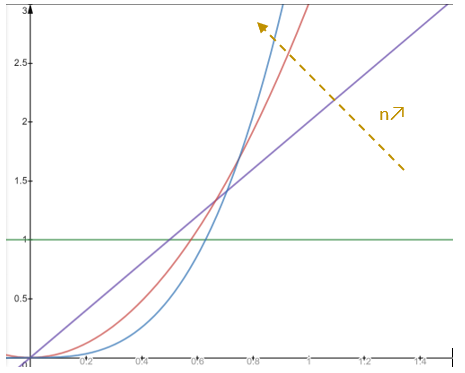
\includegraphics[scale = 0.6]{synthese_cm12_1.jpg}
        \end{figure}
    \end{minipage}
\end{example}

\begin{example}
    \begin{minipage}[c]{.55\linewidth}
        \begin{equation*}
            \begin{array}{c}
                \lim\limits_{n\to\infty}\int_0^1(1-x^{2n})nx^{n-1}dx=\lim\limits_{n\to\infty}\int_0^1(1-y^2)dy=\frac{2}{3}\\[0.4cm]
                \neq\\[0.4cm]
                \int_0^1\lim\limits_{n\to\infty}(1-x^{2n})nx^{n-1}dx=0
            \end{array}
        \end{equation*}
    \end{minipage}
    \begin{minipage}[c]{.4\linewidth}
        \begin{figure}[H]
            \centering
            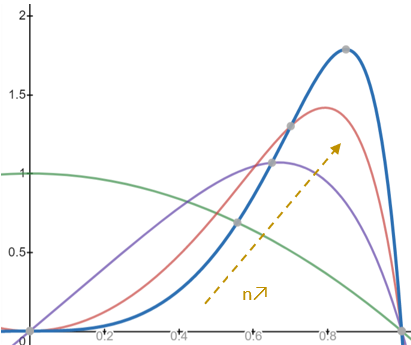
\includegraphics[scale = 0.6]{synthese_cm12_2.jpg}
        \end{figure}
    \end{minipage}
\end{example}

\begin{example}
    \begin{equation*}
        \lim_{n\to\infty}\int_{-\infty}^{+\infty}\frac{1}{1+(x-n)^2}dx=\lim_{n\to\infty}\int_0^1\frac{1}{1+y^2}dy=\pi \quad \neq\quad\int_{-\infty}^{+\infty}\lim_{n\to\infty}\frac{1}{1+(x-n)^2}dx=0
    \end{equation*}
    \begin{figure}[H]
        \centering
        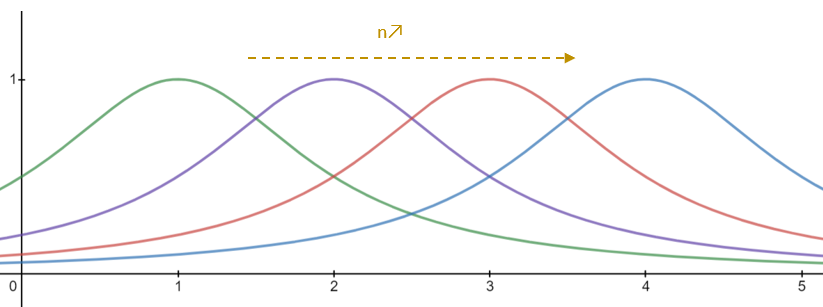
\includegraphics[scale = 0.6]{synthese_cm12_3.jpg}
    \end{figure}
\end{example}

\begin{example}
    \begin{equation*}
        \lim_{n\to\infty}\int_{-\infty}^{+\infty}\frac{n}{n^2+x^2}dx=\lim_{n\to\infty}\int_0^1\frac{1}{1+y^2}dy=\pi \quad\neq\quad\int_{-\infty}^{+\infty}\lim_{n\to\infty}\frac{n}{n^2+x^2}dx=0
    \end{equation*}
    \begin{figure}[H]
        \centering
        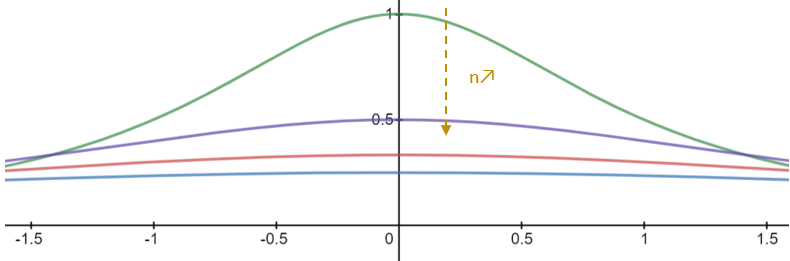
\includegraphics[scale = 0.6]{synthese_cm12_4.jpg}
    \end{figure}
\end{example}

\begin{theo}[Convergence monotone]
    Si $\forall n\in\mathbb{N}$, la fonction $f_n:X\to[0,\infty]$ est mesurable, $f_n\leq f_{n+1}$ partout sur $X$ et si $(f_n)_{n\in\mathbb{N}}$ converge ponctuellement vers $f$, alors $f$ est mesurable et on a
    \begin{equation*}
        \lim\limits_{n\to\infty}\int_A f_nd\mu = \int_Afd\mu.
    \end{equation*}
    \begin{figure}[H]
        \centering
        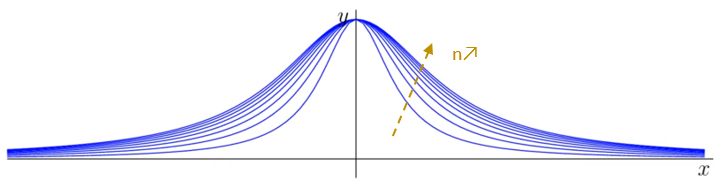
\includegraphics{synthese_conv_monotone.PNG}
    \end{figure}
\end{theo}
\begin{proof}
    On remarque tout d'abord que la suite $\big(\int_Af_nd\mu\big)_{n\in\mathbb{N}}$ est croissante et tend vers $\alpha\in[0,\infty]$. Puisque $f_n\leq f$, on sait que $\int_Af_nd\mu\leq\int_Afd\mu$ donc $\alpha\leq\int_Afd\mu$.
    
    On considère maintenant une fonction simple $s$ telle que $s\leq f$ et on pose $\theta\in]0,1[$. On définit ensuite l'ensemble $A_n=\{x\in A\big|f_n(x)\geq\theta s(x)\}$. Ces ensembles sont construits de manière à obtenir $A_n\subseteq A_{n+1}$ et $\bigcup_{n\in\mathbb{N}}A_n=A$. On observe donc que $\alpha\geq\int_Af_nd\mu\geq\int_{A_n}f_nd\mu\geq\int_{A_n}\theta sd\mu$. En faisant tendre $\theta$ vers $1$, on obtient que $\int_Asd\mu\leq\alpha$. Cette inégalité étant valable pour toute fonction simple, elle l'est aussi pour le supremum et on obtient finalement $\int_A fd\mu\leq\alpha$.
\end{proof}

\begin{theo}[Convergence dominée]
    Si $\forall n\in\mathbb{N}$, la fonction $f_n:X\to\mathbb{C}$ est telle que $(f_n)_{n\in\mathbb{N}}$ converge ponctuellement vers $f$ et si $\exists g:X\to[0,\infty[$ est intégrable sur $A$ et qu'on a la relation $|f_n|\leq g\ \forall n\in\mathbb{N}$, alors $f$ est intégrable et on a
    \begin{equation*}
        \lim\limits_{n\to\infty}\int_A f_nd\mu = \int_Afd\mu.
    \end{equation*}
    \begin{figure}[H]
        \centering
        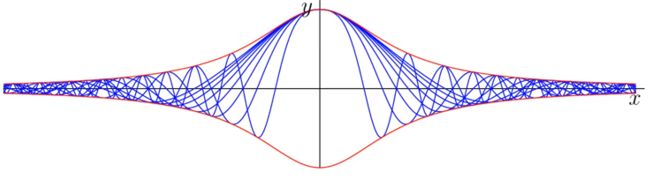
\includegraphics{synthese_conv_dominee.PNG}
    \end{figure}
    (comme $g$ est intégrable, l'aire sous sa courbe est finie et les fonctions $f_n$ doivent rester dans une partie du plan qui est finie)
\end{theo}
\begin{proof}
    Pour démontrer ce théorème, on va considérer des fonctions $f_n:X\to\mathbb{R}$.
    
    On définit pour chaque $n\in\mathbb{N}$ $\underbar{f}_n = \inf_{k\geq n}f_k$ et $\bar{f}_n = \sup_{k\geq n}f_k$. D'après le théorème de la convergence monotone, on a que $\lim\limits_{n\to\infty}\int_A\underbar{f}_n+g\ d\mu = \int_Af+g\ d\mu$ et $\lim\limits_{n\to\infty}\int_Ag-\bar{f}_n\ d\mu = \int_Ag-f\ d\mu$. Dès lors, $\lim\limits_{n\to\infty}\int_A\underbar{f}_nd\mu = \int_Afd\mu=\lim\limits_{n\to\infty}\bar{f}_nd\mu$. Grâce au théorème de l'étau, il est possible de conclure que $\lim\limits_{n\to\infty}\int_Af_nd\mu=\int_Afd\mu$.
\end{proof}

\begin{theo}[Réciproque de la convergence dominée]
    Si on a une suite de fonction $f_n:X\to[0,\infty[\ \forall n\in\mathbb{N}$ telle que $(f_n)_{n\in\mathbb{N}}$ converge ponctuellement vers $0$, et si $\lim\limits_{n\to\infty}\int_A f_nd\mu=0$, alors, $\exists g:X\to[0,\infty[$ intégrable sur $A$ et $\exists$ un suite strictement croissante $(n_k)_{k\in\mathbb{N}}$ dans $\mathbb{N}$ telle que $\forall k\in\mathbb{N}$, on ait $|f_{n_k}|\leq g$.
\end{theo}

\section{Différentiation et transformation de mesures}
\begin{theo}
    Si $f:X\to[0,\infty[$ est Borel-mesurable et si $\mu:\mathscr{B}(X)\to[0,\infty]$ est une mesure, alors $\nu:X\to[0,\infty]$ définie pour $A\in\mathscr{B}(X)$ par
    \begin{equation*}
        \nu(A)=\int_Afd\mu
    \end{equation*}
    est une mesure.
\end{theo}
\begin{proof}
    On remarque tout d'abord que $\nu(\emptyset)=\int_\emptyset fd\mu=0$.
    
    Ensuite, si on prend $A_n\in\mathscr{B}(X)$ disjoint, on a
    \begin{equation*}
        \nu\left(\bigcup_{n\in\mathbb{N}}A_n\right) = \int_{\bigcup_{n\in\mathbb{N}}A_n}fd\mu=\sum_{n\in\mathbb{N}}\int_{A_n}fd\mu = \sum_{n\in\mathbb{N}}\nu(A_n)
    \end{equation*}
\end{proof}

\begin{definition}
    Une mesure $\mu:Y\to[0,\infty]$ ($Y\in X$ est une $\sigma$-algèbre) est \textbf{$\sigma$-finie} si $\exists$ des ensembles $A_n\in Y$ tels qu'on peut écrire $X=\bigcup_{n\in\mathbb{N}}A_n$ avec $\mu(A_n)<\infty$.
\end{definition}

\begin{theo}[Radon-Nikodym]
    Si $\mu:\mathscr{B}(X)\to[0,\infty]$ est une mesure $\sigma$-finie et si $\nu:\mathscr{B}(X)\to[0,\infty]$ est absolument continue par rapport à $\mu$ ($\mu(A)=0\implies\nu(A)=0$), alors il existe une unique fonction $f:X\to[0,\infty]$ telle que $\forall A\in\mathscr{B}(X)$ on ait
    \begin{equation*}
        \nu(A)=\int_Afd\mu.
    \end{equation*}
    La fonction $f$ est appelée \textbf{dérivée de Radon-Nikodym} et est notée $\frac{d\nu}{d\mu}$. 
\end{theo}

\begin{remark}
    La continuité absolue est une hypothèse essentielle.
\end{remark}
\begin{example}
    Prenons $\mu=\lambda^1$, la mesure de Lebesgue sur $\mathbb{R}$ et $\nu$ la mesure de Dirac en $0$. Dès lors,
    \begin{equation*}
        \nu(\{0\}) = 1 \quad \neq \quad \int_{\{0\}}fd\mu=0
    \end{equation*}
    avec $f:X\to[0,\infty]$.
\end{example}

\begin{remark}
    La $\sigma$-finitude absolue est une hypothèse essentielle.
\end{remark}
\begin{example}
    Prenons $\mu$ la mesure de comptage ($\mu(A)=\#A=$ cardinal de $A=$ nombre d'éléments dans $A$) et $\nu=\lambda^1$ la mesure de Lebesgue. Dès lors, il devrait exister $a\in\mathbb{R}$ tel que $f(a)>0$ et on a alors $f(a)=\int_{\{a\}}fd\mu$ d'après la mesure $\mu$ or d'après la mesure $\nu=\int_{\{a\}}fd\mu$ on trouverais $0$...
\end{example}

\begin{definition}
    Si la fonction $f:X\to Y$ est Borel-mesurable et si $\mu:\mathscr{B}(X)\to[0,\infty]$ est une mesure, on définit la \textbf{mesure image} $f_*\mu:\mathscr{B}(Y)\to[0,\infty]$ par
    \begin{equation*}
        f_*\mu(A)=\mu\left(f^{-1}(A)\right)
    \end{equation*}
\end{definition}
\begin{proof}
    Tout d'abord, on remarque que cette fonction est bien définie car $f^{-1}(A)\in\mathscr{B}(X)$ si $A\in\mathscr{B}(Y)$.
    
    Ensuite, on vérifie que c'est bien une mesure :
    \begin{itemize}
        \item $f_*\mu(\emptyset)=\mu\big(f^{-1}(\emptyset)\big)=\mu(\emptyset)=0$ ;
        \item Considérons les ensembles $A_N\in\mathscr{B}(Y)$ disjoints,
        \begin{equation*}
            f_*\mu\left(\bigcup_{n\in\mathbb{N}}A_n\right)=\mu\left(f^{-1}\left(\bigcup_{n\in\mathbb{N}}A_n\right)\right)=\mu\left(\bigcup_{n\in\mathbb{N}}f^{-1}(A_n)\right) = \sum_{n\in\mathbb{N}}\mu\big(f^{-1}(A_n)\big) = \sum_{n\in\mathbb{N}}f_*\mu(A_n)
        \end{equation*}
    \end{itemize}
\end{proof}

\begin{example}
    Définissons $\mu$ par
    \begin{equation*}
        \mu(A) = \left\{\begin{array}{ll}
            1 & \text{si $a\in A$} \\
            0 & \text{sinon}
        \end{array}\right.
    \end{equation*}
    En utilisant la définition de la mesure image, on trouve
    \begin{equation*}
        f_*\mu(A) = \left\{\begin{array}{ll}
            1 & \text{si $a \in f^{-1}(A)$ ou encore si $f(a)\in A$} \\
            0 & \text{sinon}
        \end{array}\right.
    \end{equation*}
    Et la mesure de Dirac qu'on avait au départ reste une mesure de Dirac.
\end{example}

\begin{theo}
    Si $f:X\to Y$ et $g:Y\to\mathbb{C}$ sont Borel-mesurable alors $g$ est intégrable sur $A\subseteq Y$ par rapport à $f_*\mu$ si et seulement si $g\circ f$ est intégrable sur $f^{-1}(A)\subseteq X$ par rapport à $\mu$ et
    \begin{equation*}
        \int_Ag\ d(f_*\mu) = \int_{f^{-1}(A)}g\circ f \ d\mu
    \end{equation*}
\end{theo}
\begin{proof}
    Si $s$ est une fonction simple, $(s\circ f)^{-1}(\{\alpha_i\}) = f^{-1}\big(s^{-1}(\{\alpha_i\})\big)$ et donc $\mu\big((s\circ f)^{-1}(\{\alpha_i\})\big)=f_*\mu\big(s^{-1}(\{\alpha_i\})\big)$.
\end{proof}

\begin{theo}
    Si $f(x)=Mx+a$ avec $M$ une matrice inversible, on a
    \begin{equation*}
        f_*\lambda^{n} = \frac{1}{|\det M|}\lambda^n
    \end{equation*}
\end{theo}
\begin{proof}
    Si $A,B\in\mathscr{B}(\mathbb{R}^n)$, on obtient en échangeant les ordres d'intégration et en effectuant des changements de variables par translation :
    \begin{align*}
        \lambda^n(A)(f_*\lambda^n)(B) &= \iint_{\mathbb{R}^n\times\mathbb{R}^n} \chi_A(x)\chi_{f^{-1}(B)}(y)\ dydx 
        = \iint_{\mathbb{R}^n\times\mathbb{R}^n} \chi_A(x)\chi_{B}(My+a)\ dydx \\
        &= \iint_{\mathbb{R}^n\times\mathbb{R}^n} \chi_A(x)\chi_{B}\big(M(y-M^{-1}x)+a\big)\ dydx \\
        &= \iint_{\mathbb{R}^n\times\mathbb{R}^n} \chi_A(x)\chi_{B}(My-x+a)\ dydx
        = \iint_{\mathbb{R}^n\times\mathbb{R}^n} \chi_A(My+a-z)\chi_{B}(z) dydz\\
        & = \iint_{\mathbb{R}^n\times\mathbb{R}^n} \chi_A\big(M(y-M^{-1}z)+a\big)\chi_{B}(z) dydz\\
        &= \iint_{\mathbb{R}^n\times\mathbb{R}^n} \chi_A(My+a)\chi_{B}(z) dydz
        = \iint_{\mathbb{R}^n\times\mathbb{R}^n} \chi_{f^{-1}(A)}(y)\chi_{B}(z) dydz\\
        & = (f_*\lambda^n)(A)\lambda^n(B)
    \end{align*}
    On en déduit donc que
    \begin{equation*}
        f_*\lambda^{n}(A) = \frac{f_*\lambda^{n}(B)}{\lambda^n(B)}\lambda^n(A).
    \end{equation*}
    Ensuite, en considérant que $M$ est une matrice diagonale, on a que l'ensemble $B$ est un pavé et on retrouve la formule énoncé plus haut. Si on considère une matrice $M$ orthogonale, on prend pour l'ensemble $B$ une boule. Dans le cas général, on remarque qu'une matrice quelconque s'écrit comme le produit de matrices orthogonales et diagonales et on retrouvera donc toujours la formule désirée.
\end{proof}

\begin{theo}
    De manière plus générale, si $f:U\to V$ est un difféomorphisme de classe $C^1$ : $f$ est continuement différentiable, inversible et $f^{-1}$ est continuement différentiable, alors on a
    \begin{equation*}
        f_*\lambda^n = \frac{1}{|\det df|\circ f^{-1}}\lambda^n
    \end{equation*}
\end{theo}

 
\end{document}
